\documentclass[11pt,a4paper]{book}

\usepackage{graphicx}
\usepackage{subfig}

\usepackage{ifpdf}
\ifpdf
\usepackage{epstopdf}
\usepackage[usenames,dvipsnames]{color}
\usepackage[pdftex,bookmarks=true,hypertexnames=false]{hyperref}
\hypersetup{
  pdfauthor = {Jing Liu},
  pdftitle = {},
  pdfsubject = {PhD Thesis},
  pdfkeywords = {neutrino, double beta decay, germanium detector},
}
\pdfadjustspacing=1
\else
\usepackage[usenames,dvips]{color}
\usepackage[ps2pdf]{hyperref}
\fi

\usepackage{amsmath}            % more evironment
\usepackage{amssymb}            % more symbol
\usepackage{simplewick}         % for wick contraction in QFT

%\usepackage{fancyhdr}
%\fancyhead{}                    %clear default settings
%\fancyfoot{}                    %clear default settings
%\fancyhead[ER]{\rightmark}
%\fancyhead[EL]{\thepage}
%\fancyhead[OL]{\leftmark}
%\fancyhead[OR]{\thepage}

\setlength{\oddsidemargin}{1cm}
\setlength{\evensidemargin}{0cm}
\setlength{\textwidth}{15cm}
\setlength{\textheight}{21cm}
\setlength{\hoffset}{0cm}
\setlength{\voffset}{0cm}

% Alter some LaTeX defaults for better treatment of floats: See p.105 % of "TeX Unbound" for suggested values. See pp. 199-200 of Lamport's % "LaTeX" book for details.

% General parameters, for ALL pages:
\renewcommand{\topfraction}{0.9} % max fraction of floats at top
\renewcommand{\bottomfraction}{0.9} % max fraction of floats at bottom

% Parameters for TEXT pages (not float pages):
\setcounter{topnumber}{2}
\setcounter{bottomnumber}{2}
\setcounter{totalnumber}{4} % 2 may work better
\renewcommand{\textfraction}{0.1} % allow minimal text w. figs

% Parameters for FLOAT pages (not text pages):
\renewcommand{\floatpagefraction}{0.7}	% require fuller float pages
% N.B.: floatpagefraction MUST be less than topfraction !!

% remember to use [htp] or [htpb] for placement


%%% Local Variables:
%%% mode:latex
%%% TeX-master: "thesis"
%%% End:


\begin{document}

\pagestyle{empty}

\begin{titlepage}

\centering

\vspace{1.0cm}
\begin{figure}[t!]
\centering
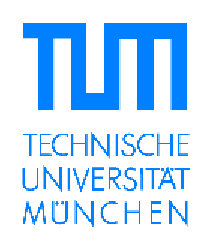
\includegraphics[height=0.12\textheight]{TUM_logo}\hfil%
\begin{minipage}[b]{0.65\textwidth}\centering
\huge Technische Universit\"at M\"unchen\\\vspace{20pt}
\large \textit{Max-Planck-Institut f\"ur Physik\\
(Werner-Heisenberg-Institut)}
\end{minipage}\hfil%
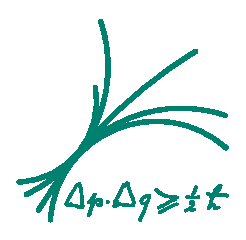
\includegraphics[height=0.12\textheight]{MPP_logo}%
\end{figure}

\vspace{1. cm}

\huge Development of Segmented Germanium Detectors for Neutrinoless Double Beta Decay Experiments

\vspace{1.5 cm}

\Large Jing Liu

\vspace{2. cm}

\normalsize Vollst\"andiger Abdruck der von der Fakult\"at f\"ur
Physik der Technischen Universit\"at M\"unchen zur Erlangung des
akademischen Grades eines \\
Doktors der Naturwissenschaften (Dr. rer. nat.) \\
genehmigten Dissertation. \\

\vspace{1.5 cm} 

\begin{table*}[h]
  \centering
  \begin{tabular}{ll}
    Vorsitzender: & Univ.-Prof. Dr. Alejandro Ibarra\\ 
    & \\ 
    Pr\"ufer der & 1. Hon.-Prof. Allen C. Caldwell, Ph.D.\\ 
    Dissertation: & 2. Univ.-Prof. Dr. Franz von Feilitzsch \\ 
  \end{tabular}
\end{table*}

\vspace{2.0 cm} 

Die Dissertation wurde am 20.04.2009 bei der Technischen Universit\"at
M\"unchen eingereicht und durch die Fakult\"at f\"ur Physik am
09.06.2009 angenommen. \\

\end{titlepage} 

\cleardoublepage

%%% Local Variables:
%%% mode:latex
%%% TeX-master: "thesis"
%%% End:


\cleardoublepage

\section*{Abstract}
The results from neutrino oscillation experiments indicate that at least two neutrinos have mass. However, what the absolute mass scale of neutrinos is and whether neutrino and anti-neutrino are their own anti-particles remain unsolved. Neutrinoless double beta decay experiments can help to improve our understanding of both problems and are the most practical method known to tackle the second question. 

The GERmanium Detector Array (GERDA) experiment searching for the neutrinoless double beta decay of $^{76}$Ge is currently under construction in Hall A of the INFN Gran Sasso National Laboratory (LNGS), Italy. In order to achieve an extremely low background level, segmented germanium detectors will be operated directly in liquid argon which serves as cooling and shielding material simultaneously. 

Several test cryostats were built to operate segmented germanium detectors in vacuum and cryogenic liquid at the Max-Planck-Institut f\"ur Physik in M\"unchen, Germany. The performance and the background discrimination power of segmented germanium detectors were studied in detail. It was proved for the first time that the segmented germanium detector can be operated directly in cryogenic liquid stably for a long period, and that the segmentation scheme employed does well in the identification of photon and neutron induced background.

A comprehensive C++ simulation framework, MaGe (Majorana-Gerda), is jointly developed by the Majorana and GERDA collaborations. It is based on Geant4, but tailored to be especially suitable for the simulation of the response of ultra-low radioactive background radiation detectors to ionizing radiation. The predictions of the simulations were verified to hold to 5\%.

Pulse shape analysis is a complementary method to segmentation for further identifying background events. Its identification efficiency needs to be estimated using reliable pulse shape simulations. A full-functional pulse shape simulation package was developed within the MaGe framework. The simulation was verified using data taken from the first segmented prototype detector for GERDA. The understanding of the properties of the segmented germanium detectors was improved meanwhile.

\clearpage


\section*{Zusammenfassung}
(google translate version)

Die Ergebnisse von Neutrino-Oszillation Experimente deuten darauf hin, dass mindestens zwei Neutrinos Masse haben. Aber was die absolute Masse des Neutrinos Massstab ist und ob Neutrino und Anti-Neutrino sind ihre eigenen Anti-Teilchen nach wie vor ungel\"ost. Neutrinoless double beta decay Experimente zur Verbesserung unseres Verst\"andnisses der Probleme und sind die praktischste Methode, um die zweite Frage.

Die GERmanium Detector Array (GERDA) Experiment der Suche nach dem neutrinoless doppelte Beta-Zerfall von $^{76}$Ge ist derzeit im Aufbau in der Halle A des INFN Gran Sasso National Laboratory (LNGS), Italien. Um eine extrem niedrige Hintergrund Ebene, segmentierten Germanium-Detektoren werden direkt in fl\"ussigem Argon die als K\"uhl-und Abschirmmaterial gleichzeitig.

Mehrere Tests Kryostaten wurden f\"ur den Betrieb segmentierten Germanium-Detektoren im Vakuum und kryogene Fl\"ussigkeit auf dem Max-Planck-Institut f\"ur Physik in M\"unchen, Deutschland. Die Leistungsf\"ahigkeit und den Hintergrund der Diskriminierung Macht der segmentierten Germanium-Detektoren wurden im Detail untersucht. Es wurde bewiesen, für die das erste Mal, dass die segmentierten Germanium-Detektor kann direkt in kryogenen Fl\"ussigkeit stabil f\"ur eine lange Zeit, und dass die Segmentierung des Systems besch\"aftigt hat auch bei der Identifizierung von Photonen-und Neutronen-induzierten Hintergrund.

Eine umfassende C++-Framework, MaGe (Majorana-Gerda), wird gemeinsam von der Majorana und GERDA Kooperationen. Es basiert auf Geant4, aber abgestimmt auf die besonders geeignet für die Simulation der Reaktion der ultra-niedrige radioaktive Strahlung Hintergrund Detektoren durch ionisierende Strahlung. Die Vorhersagen der Simulationen wurden \"uberpr\"uft, um zu 5 \%.

Pulsform-Analyse ist eine erg\"anzende Methode zur Segmentierung für die weitere Ermittlung Hintergrund Veranstaltungen. Die Ermittlung der Effizienz muss anhand zuverl\"assiger Pulsform Simulationen. Eine vollst\"andige funktionelle Pulsform Simulation Paket wurde entwickelt, in der Magier Rahmen. Die Simulation wurde \"uberpr\"uft anhand der Daten aus den ersten Prototyp segmentierten Detektor f\"ur Gerda. Das Verst\"andnis f\"ur die Eigenschaften der segmentierten Germanium-Detektoren wurde inzwischen verbessert.

\clearpage

%%% Local Variables:
%%% mode:latex
%%% TeX-master: "thesis"
%%% End:


\cleardoublepage \setcounter{page}{1} \pagenumbering{Roman}

\tableofcontents

\cleardoublepage \setcounter{page}{1} \pagenumbering{arabic}

\pagestyle{headings}

\chapter{Introduction}
\label{cha:intro}
%$Id$
At the time the \emph{Standard Model} was established the neutrino was
believed to be massless. In experiments it always had the same
chirality and there was no evidence for a non-zero mass. However, the
picture changed dramatically when neutrino oscillations were observed
in solar and atmospheric neutrinos. They are explained by the weak
interaction eigenstates of neutrinos being admixture of mass
eigenstates and the latter propagating with different velocities. The
introduction of neutrino mass terms into the \emph{Standard Model}
becomes necessary.

There are various methods to introduce the mass terms of neutrinos
into the \emph{Standard Model}. The most straightforward approach is
to follow the same procedure as for the electron, \textit{i.e.} the
lepton obtains mass by coupling to the Higgs field. The problems of
this approach are, that it does not explain why neutrinos couple to
the Higgs field so weakly compared with their leptonic partners, and
that it requires the introduction of right-handed neutrinos which are
not observed yet in the experiment. An elegant way to solve these
problems is to assume that neutrinos are Majorana particles,
\textit{i.e.} their own anti-particles. This way, the second problem
does not arise, and once the Majorana mass terms are introduced into
the Lagrangian the so-called \emph{see-saw mechanism} can make the
different coupling strengths look natrual.

Different theoretical and experimental methods are under investigation to verify that neutrinos are Majorana particles. The only experimental evidence for a Majorana nature of the neutrino for the time being would be neutrinoless double beta decay ($0\nu\beta\beta$). In this process, a neutrino emitted from one beta decay is absorbed by another beta decay. This can only happen if neutrinos are of Majorana type. Ten naturally occurring isotopes are observed to have double-beta decay. Among them $^{76}Ge$ is of special importance because, at first, germanium is a semiconductor material and can be made into detectors with very good energy resolution, it can serve as source and detector simultaneously, the efficiency of detection is very high, secondly, germanium is the purest material that can be produced in the world, the intrinsic background source is very limited.

The GERDA (GERmanium Detector Array) experiment searching for
$0\nu\beta\beta$ decay of $^{76}Ge$ is currently under
construction in Hall A of the INFN Gran Sasso National Laboratory
(LNGS), Italy. In order to achieve an extremely low background index
in the second phase of GERDA 18-fold segmented germanium detectors
will be operated directly in cryogenic liquid serving as cooling and
shielding material. The main goal of this thesis is to examine
systematically the operation and performance of segmented detectors in
cryogenic liquid, and to investigate their power of background
discrimination by analyzing the spatial distribution over which energy
is deposited and the time structure of the detector response.

Several test facilities were built:\\
\emph{Siegfried}, an 18-fold segmented prototype detector for GERDA
Phase II was operated in a traditional cryostat. This allowed
\begin{itemize}
\item the characterization of the prototype detector and its
  electronics, including the resolutions, cross talks, segment
  boundaries, crystal axes and impurities, \textit{etc}.
\item the analysis of background induced by external photons in the
  MeV-energy range. These photons typically undergo multiple Compton
  scattering and deposit their energy over a range of several
  centimeters. This distinguishes them from the electrons from
  $0\nu\beta\beta$ decay which deposit energy on a millimeter
  scale.
\item the analysis of background induced by neutron interactions with
  germanium isotopes and surrounding materials. Most of the neutron
  induced events deposit energy in different segments of the detector.
  Particularly, the neutron inelastic scattering on germanium isotopes
  is of great interest because of the entanglement of the nuclear
  recoil energy and the prompt photon energy.
\end{itemize}
\emph{Gerdalinchen II}, a specially designed cryostat containing
liquid nitrogen or argon, inside which different types of detectors
were operated, was used to carry out the following studies:
\begin{itemize}
\item the operation of several segmented detectors submerged directly
  in cryogenic liquid. Detailed operating procedures were
  investigated. The performance of the detectors was carefully
  monitored and analyzed.
\item the scanning of the prototype detectors. This data was used to
  study the time structure of the detector response, \textit{i.e.}
  pulse shape. A reliable pulse shape simulation package was developed
  and verified by being compared with data.
\item two neutron experiments with improved shielding. The influence
  of neutron interactions with cryogenic liquid on the detector was
  examined. The Monte Carlo simulation of low energy neutron
  interactions was verified in detail.
\end{itemize}
Different pulse shape analyses were carried out based on the data from
different test stands and the simulation.

The content of the thesis is summarized as following:
\begin{description}
\item[Chapter 2] describes the theoretic background of   $0\nu\beta\beta$ decay, and other approaches to check whether   neutrinos are of Majorana type or Dirac type.
\item[Chapter 3] introduces the basic ideas of the GERDA experiment,
  summarizes the latest results of $0\nu\beta\beta$ decay from
  previous experiments, compares GERDA with competitive experiments
  and estimates the potential of future $0\nu\beta\beta$ decay
  experiments.
\item[Chapter 4] summarizes the basic concepts of semiconductor
  detectors and the important properties of germanium crystals and
  detectors related to the later analysis
\item[Chapter 5] introduces the two test stands that provided the data
  for all studies, describes the slow control and data acquisition
  system relying on which the test stands were running.
\item[Chapter 6] characterizes the short and long term performance of
  segmented germanium detectors in cryogenic liquid test stand.
\item[Chapter 7] demonstrates the power of the segmented detectors to
  identify different kinds of background, especially introduced by
  neutron interactions with germanium isotopes and surrounding
  materials.
\item[Chapter 8] describes the methods to simulate the pulse shapes of
  different types of interactions in germanium detectors, verifies the
  simulation by comparing it with the measurements.
\item[Chapter 9] further classifies the background events by using
  different pulse shape analysis methods , compares them to each
  other, and investigates the power of integrating pulse shape
  analysis with the analysis based on the detector segmentation.
\item[Chapter 10] summarizes all the studies in the concept of the
  GERDA Phase II experiment, discusses the meanings of the studies for
  GERDA, and gives a outlook on further studies.
\end{description}

%%% Local Variables:
%%% mode:latex
%%% TeX-master: "thesis"
%%% End:

\clearpage{\pagestyle{empty}\cleardoublepage}

\chapter{Neutrino mass and its origin}
\label{cha:theory}
Neutrinos were introduced into the \emph{Standard Model} as massless particles. But strong evidences from neutrino oscillations experiments showed that at least one of the neutrinos had mass. In order to include neutrino mass into the \emph{Standard Model} without conflicting with the fact that neither right handed neutrinos nor left handed anti-neutrinos are observed, neutrinos are assume to be of Majorana type, \textit{i.e.} their own anti-particles. Neutrinoless double beta decay would exist only if this assumption is true. And from the rate of Neutrinoless double beta decay the effective Majorana neutrino mass can be deduced. This can help to solve the neutrino mass hierarchy problem that cannot be solved by the neutrino oscillation experiment alone. There are approaches other than neutrinoless double beta decay which can also address on the same problem. But they are not quite practical for the time being.

\section{Neutrinos in \emph{Standard Model}}
\label{sec:sm}
In the \emph{Standard Model} neutrinos are assumed to be fermions with spin 1/2 and rest mass $m_\mu=0$. They always have fixed helicities because there is no frame of reference moving faster than a neutrino, where the helicity of the neutrino could change its sign. Neutrinos and anti-neutrinos are believed to be different particles. Lepton numbers +1 and -1 are assigned to them respectively and the sum of which is required to be conservative in order to indicate the difference. Only left-handed neutrinos and right-handed anti-neutrinos participate the weak interaction. The field operators of right-handed neutrinos and left-handed anti-neutrinos do not present in the Lagrangian density of weak interaction at all.

New experimental evidences, particularly neutrino oscillations, make the modification and extension of the \emph{Standard Model} necessary. Crucial theoretical considerations and experimental observations of neutrinos in history leading to the above statements are briefly reviewed below in order to investigate the space allowed for new ideas.

The neutrino was postulated to exist by W. Pauli in 1930 in order to explain the continuous energy spectrum of electrons emitted from the beta decay without abandoning the law of energy conservation. He assumed that it was a neutral fermion with spin 1/2, and its mass was of the same order of magnitude as the electron mass.~\cite{Pau30} E. Fermi soon developed his theory of beta decay according to the beta spectrum~\cite{Fer33,Fer34}. He investigated the influence of the neutrino mass on the shape of beta spectrum and inferred that $m_\nu \approx 0$ by comparing the calculation with the experimental data. A precise measurement of the beta spectrum of tritium by L. Langer and R. Moffat in 1952~\cite{Lan52} gave an upper limit on the rest mass of the neutrino, $m_\nu < 250 \mbox{eV} = 0.002m_e$. The neutrino was assumed to be massless afterwards. Although the upper limit was pushed down again and again by the later experiments, the possibility that neutrinos have very tiny masses have never been completely ruled out.

Beta plus decay was observed in artificial radioactivity by Joliot and Curie nearly around the same period. Conventionally, beta decay and beta plus decay are noted as follows:
\begin{equation}
  \label{eq:bd}
  \beta\mbox{-decay: } n \rightarrow p+e^{-}+\bar{\nu}_e
\end{equation}
\begin{equation}
  \label{eq:bpd}
  \beta^+\mbox{-decay: energy} + p \rightarrow n+e^{+}+\nu_e
\end{equation}
If $\bar{\nu}$ and $\nu$ are the same the following reaction could happen:
\begin{equation}
  \label{eq:bnun}
  \bar{\nu}_e + n \rightarrow p+e^{-}
\end{equation}
This was investigated by R. Davis in 1955~\cite{Dav55,Dav56}. In the real experiment Davis was looking for
\begin{equation}
  \label{eq:bnucl}
  \bar{\nu}_e + ^{37}\mbox{Cl} \rightarrow ^{37}\mbox{Ar}+e^{-}
\end{equation}
and gave a negative result. From then on, $\bar{\nu}$ and $\nu$ were believed to be different particles. To formulate this idea theoretically different \emph{lepton numbers} were assigned to $e^{-}, e^{+}, \nu_e$ and $\bar{\nu}_e$:
\begin{equation}
  \label{eq:ln}
  +1 \mbox{ for }e^{-}, \nu_e, \mbox{   }-1 \mbox{ for }e^{+},\bar{\nu}_e,
\end{equation}
and required to be conservative in the interaction. Eq. \ref{eq:bnucl} could not happen because the \emph{lepton number} was different before and after the reaction. However, after parity violation in weak interaction was observed the same phenomenon was no longer necessarily to be elaborated in this way.

In 1956 T. D. Lee and C. N. Yang found the existing evidence of parity conservation in weak interaction unsatisfactory and specified the experiments required to check it.~\cite{Lee56} Soon after that the parity violation was observed in the beta decay of $^{60}$Co~\cite{Wu57} and the creation and decay of muons~\cite{Gar57,Fri57}. Lee and Yang~\cite{Lee57} and some other authors~\cite{Sal57,Lan57} started to apply the so-called two-component model~\cite{Wey29} to the weak interaction. According to this model only the left-handed neutrino and right-handed anti-neutrino or right-handed neutrino and left-handed anti-neutrino participate the weak interaction. In 1958 an elegant experiment was carried out by M. Goldhaber \textit{et al.} to see whether the right-handed or left-handed components were preferred by nature.~\cite{Gol58} By measuring the polarization of $\gamma$-rays emitted from $^{152}$Sm* created in the electron capture $^{152}$Eu$(e^-,\nu)$ they inferred that neutrinos from $^{152}$Eu$(e^-,\nu)$ were left-handed. Now the absence of reaction \ref{eq:bnucl} can be explained in two different ways:
\begin{itemize}
\item $\bar{\nu}$ and $\nu$ are intrinsically different particles.
\item $\bar{\nu}$ and $\nu$ are the same particles with different
  helicities. It is the latter that causes the different behaviors of
  $\bar{\nu}$ and $\nu$.
\end{itemize}

To sum up, though the \emph{Standard Model} of weak interaction is a very successful theory the modifications of some of its statements are not totally impossible. Two points important to the following discussion are summarized here:
\begin{itemize}
\item neutrinos are not necessarily to be massless;
\item $\bar{\nu}$ and $\nu$ might be the same, and hence the
  \emph{lepton number} does not need to be conservative.
\end{itemize}


\section{Neutrino oscillations}
\label{sec:osci}
Different voices always existed parallel to the development of the \emph{Standard Model} that we have today. The assumption that neutrinos were massless was challenged long time ago. Early in 1969 Gribov and Pontecorvo predicted that neutrinos might oscillated into different flavors if some of them were massive and if there was mixing between them.~\cite{Gri69} This is what we call today \emph{neutrino oscillations}.

The theory of \emph{neutrino oscillations} can be briefly summarized as follows: the mass eigenstates of neutrinos are not the same as their weak interaction eigenstates; the latter is a combination of the former
\begin{equation}
  \label{eq:osci}
  |\nu_{\alpha}\rangle=\sum_{i}U^{*}_{\alpha i}|\nu_{i}\rangle,
\end{equation}
where $\alpha=e,\mu,\tau$, $i=1,2,3$, and $U$ is a unitary matrix referred to as the Pontecorvo-Maki-Nakagawa-Sakata(PMNS) matrix. A common parameterization of PMNS matrix is
\begin{eqnarray*}
  \label{eq:pmns}
  U = \left(\begin{array}{ccc}
      1 & 0 & 0 \\ 0 & C_{23} & S_{23} \\ 0 & -S_{23} & C_{23}
    \end{array}\right) &\times&
  \left(\begin{array}{ccc}
      C_{13} & 0 & S_{13}e^{-i\delta} \\ 
      0 & 1 & 0 \\ -S_{13}e^{-i\delta} & 0 & C_{13}
    \end{array}\right) \\\times
  \left(\begin{array}{ccc}
       C_{12} & S_{12} & 0 \\ -S_{12} & C_{12} & 0 \\ 0 & 0 & 1
    \end{array}\right) &\times&
  \left(\begin{array}{ccc}
      e^{i\alpha_1/2} & 0 & 0 \\ 0 & e^{i\alpha_2/2} & 0 \\ 0 & 0 & 1
    \end{array}\right),
\end{eqnarray*}
where $S_{ij} = \sin\theta_{ij}$, $C_{ij} = \cos\theta_{ij}$ represent the sines and coines of the three mixing angles, $\delta, \alpha_1$ and $\alpha_2$ are CP-violating phasees. Taking two generations as an example, eq.~\ref{eq:osci} can be expressed as
\begin{equation}
  \label{eq:osci2}
  \left(\begin{array}{c}\nu_{\alpha}\\\nu_{\beta}\end{array}\right)=
  \left(\begin{array}{cc} \cos\theta & \sin\theta\\
      -\sin\theta & \cos\theta \end{array}\right)
  \left(\begin{array}{c}\nu_{1}\\\nu_{2}\end{array}\right).
\end{equation}
The probability for the neutrino to change flavor after traveling a distance $L$, $p(\nu_\alpha \rightarrow \nu_\beta)$, is
\begin{equation}
  \label{eq:pa2b}
  p(\nu_\alpha \rightarrow \nu_\beta)=
  \sin^{2}2\theta\sin^{2}\left(\Delta m^{2}_{12}\frac{L}{4E}\right),
\end{equation}
where $\Delta m^{2}_{12}$ is the squared mass difference between the two mass eigenstates $|m^{2}_{1} - m^{2}_{2}|$, while $E$ is the average energy of the mass eigenstates.

There would be not oscillation ($p(\nu_\alpha \rightarrow \nu_\beta) = 0$), if neutrinos are all massless ($\Delta m^{2} = 0$) or not mixing ($\theta = 0$), \textit{i.e.} if there are neutrino oscillations at least one of the neutrinos has mass and there is mixing between them.

\subsection{Atmosphere neutrinos}
\label{sec:atmo}
The hypothesis of neutrino oscillations was at first used to explain the problem of the solar neutrino flux~\cite{Dav64,Dav68}, which was smaller than that was predicted by the standard solar model~\cite{Bah98}. This explanation was not widely accepted because it required very large neutrino mixing and a fine-tuned mass difference squared to fit the distance between the Sun and the Earth. The uncertainties of the standard solar model could be used to solve this problem as well.

The studies of the atmosphere neutrinos, however, presented the first evidence of neutrino oscillations. In the early 1980s, several massive detectors were built to search for proton decays. Neutrinos created by the cosmic rays in the atmosphere were studied in detail as background events. A deficit in the muon neutrino flux relative to the electron neutrino flux compared with the calculation was found in two experiments, IMB~\cite{Hai86} (1986) and Kamiokande~\cite{Hir88} (1988). The IMB group, however, took the conservative attitude that this deficit is probably ascribable to some unknown systematics. On the other hand, the Kamiokande, relying on its capability for clear $e, \mu$ event separation, ventured to interpret it as a result of neutrino oscillation.

Kamiokande further investigated this problem and found that higher energy muon neutrino flux showed a nontrivial zenith-angle dependence that could be explained by $\nu_\mu$ oscillating to $\nu_\tau$ in 1994.~\cite{Fuk94} This still did not convinced everybody because the oscillation interpretation required very large mixing between two neutrinos, which did not look reasonable. Finally, Super-Kamiokande, the enlarged facility of Kamiokande, showed that every aspects of atmosphere neutrino data were consistent with neutrino oscillation between $\nu_\mu$ and $\nu_\tau$, and the mixing was nearly maximal (1998).~\cite{Fuk98}

\subsection{Solar neutrinos}
\label{sec:solar}
The hypothesis of neutrino oscillations was not taken seriously as a solution of the solar neutrino puzzle until Mikheyev and Smirnov brought up an idea in 1986 that $\nu_e$s could be efficiently converted into $\nu_mu$s when passing through the matters on the surface of the Sun.~\cite{Mik86} This mechanism did not require the intrinsic mixing angle to be very large and the fine-tuned mass difference squared to fit the distance between the Sun and the Earth. This is the so-called MSW effect~\cite{Mik86,Wol78}.

The experimental evidences of solar neutrino deficit coming after~\cite{Hir89,Aba91,Ans92} were all explained as the result of neutrino oscillations and the ranges of allowed neutrino mixing parameters were narrowed down step by step. The neutrino oscillations was finally confirmed by the combined results from the Sudbury Neutrino Observatory (SNO) and Super-Kamiokande (2001)~\cite{Ahm01,Fuk01}. SNO measured the $^8$B solar neutrinos through the reactions
\begin{eqnarray*}
  \nu_e + d \rightarrow p + p + e^- &\mbox{\ \ \ \ \ \ (CC)}&,\\
  \nu_\alpha + d \rightarrow p + n + \nu_\alpha &\mbox{\ \ \ \ \ \     (NC)}&,\\
  \nu_\alpha + e^- \rightarrow \nu_\alpha + e^- &\mbox{\ \ \ \ \ \     (ES)}&.
\end{eqnarray*}
The charged current (CC) reaction is sensitive exclusively to $\nu_e$, while the neutral current (NC) and the elastic scattering (ES) are sensitive to all active neutrino flavors ($\alpha = e, \mu, \tau$). If $\nu_e$s from the Sun change into other flavors, the neutrino flux measured from CC interaction, $\phi^{CC}(\nu_e)$, should be smaller than that from ES interaction, $\phi^{ES}(\nu_\alpha)$. It turned out that $\phi^{CC}(\nu_e)$ measured by SNO was smaller than $\phi^{ES}(\nu_\alpha)$ precisely measured by Super-Kamiokande with a $3.3\sigma$ difference. This is a very convincing evidence of neutrino oscillations because it does not rely on solar model flux calculations.

\subsection{Summary of experimental results}
\label{sec:allo}
Neutrino oscillations have been observed not only in solar and atmosphere neutrino experiments but also in reactor~\cite{Ara05} and accelerator~\cite{Dod06,Agu07} neutrino experiments. It is confirmed that neutrinos do have masses. Comprehensive data analyses of the squared-mass differences and the mixing parameters based on the 3-neutrino mixing scheme can be found in the latest \emph{Review of   Particle Physics}~\cite{PDG07}. The results are listed in Table~\ref{tab:par}. The mass difference squared, $m^{2}_{12}$, is mainly from the data of solor neutrino oscillations, $m^{2}_\odot$; while the mass difference squared, $m^{2}_{23}$, is mainly from the data of atmosphere neutrino oscillations, $m^{2}_{\mbox{atm}}$. Since the solor and atmosphere neutrino oscillations experiments can only measure the mass difference of the neutrino mass eigenstates and cannot determine the signs of $m^{2}_{12}$ and $m^{2}_{23}$, there are two interesting questions left as shown in Fig~\ref{fig:hie}
\begin{itemize}
\item what are the absolute values of neutrino masses?
\item what is the real mass hierarchy? Is it the same as their lepton partners, namely, the normal hierarchy, or the inversed heirarchy, as shown in Fig~\ref{fig:hie}
\end{itemize}
\begin{figure}[tbhp]
  \centering
  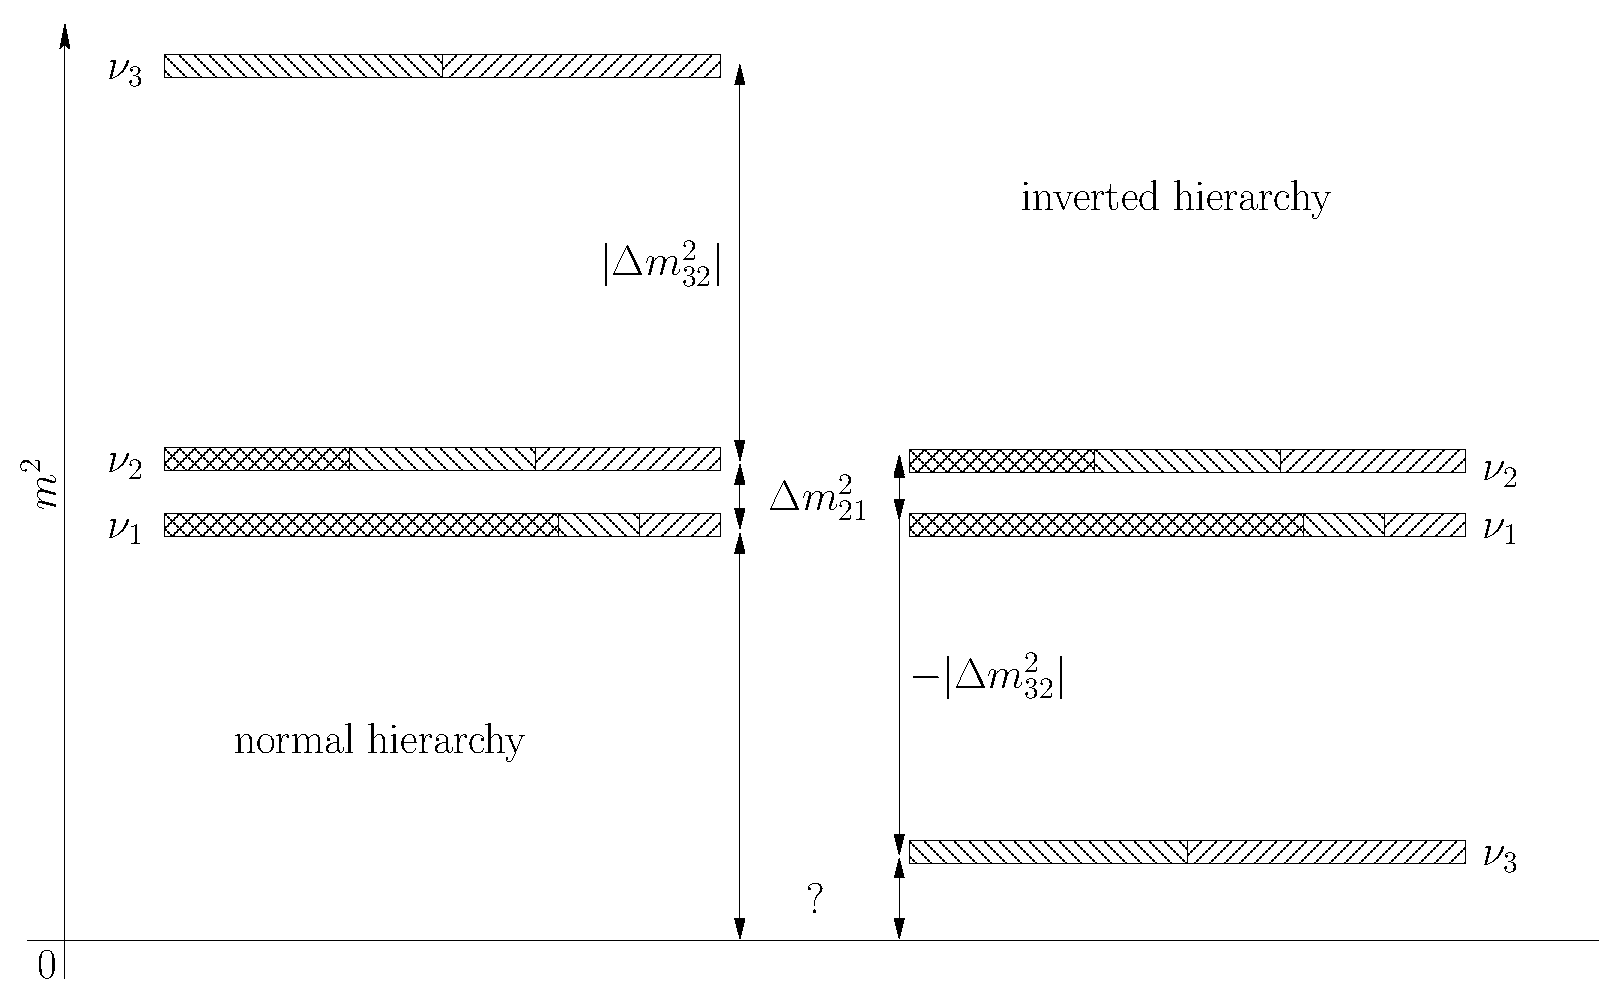
\includegraphics[width=0.8\textwidth]{massHierarchy.eps}  
  \caption{Possible neutrino squared-mass spectra. Oscillation     experiments can neither tell how far above zero the entire spectra     lie, nor the real mass hierarchy.}
  \label{fig:hie}
\end{figure}

\begin{table}[tbhp]
  \centering
  \caption{Summary of the neutrino squared-mass differences and the             mixing parameters based on the 3-neutrino mixing scheme. The suffixes         $_\odot$ and $_{\mbox{atm}}$ stand for the results from solar and         atmosphere experiments, respectively.}
  \label{tab:par}
  \begin{tabular}{lr}\hline\hline
    Parameter & Value \\\hline
    $\sin^{2}2\theta_{12} \approx \sin^{2}2\theta_{\odot}$ &     $0.86^{+0.03}_{-0.04}$ \\
    $\sin^{2}2\theta_{23} \approx \sin^{2}2\theta_{\mbox{atm}}$ &         $>0.92$ (C.L. = 90\%) \\
    $\sin^{2}2\theta_{13}$ & $<0.19$ (C.L. = 90\%) \\
    $\Delta m^{2}_{21}~[10^{-5}\mbox{eV}^{2}]$ & $0.8 \pm 0.3$ \\
    $|\Delta m^{2}_{32}|~[10^{-3}\mbox{eV}^{2}]$ & 1.9 to 3.0         \\\hline\hline
  \end{tabular}
\end{table}

\section{Dirac neutrinos}
\label{sec:dirac}
The observation of neutrino oscillations makes the introduction of neutrino mass terms into the \emph{Standard Model} necessary. In case of free fields of fermions, the Dirac equation can be deduced from the Lagrangian density
\begin{equation}
  \label{eq:deq}
  \mathcal{L} = \bar{\psi} (i\gamma^{\mu}\partial_{\mu}-m) \psi,
\end{equation}
where $\psi$ is the free Dirac field. The first term corresponds to the kinetic energy and the second is the Dirac mass term,
\begin{equation}
  \label{eq:dm}
  \mathcal{L}_D=m_{D}\bar{\psi}\psi.
\end{equation}
Since
\begin{equation}
  \label{eq:deq}
  \bar{\psi}\psi =  \bar{\psi}     \left(\frac{1+\gamma^5}{2}+\frac{1-\gamma^5}{2}\right)
  \left(\frac{1+\gamma^5}{2}+\frac{1-\gamma^5}{2}\right) \psi =
  \bar{\psi}_{L}\psi_{R}+\bar{\psi}_{R}\psi_{L},
\end{equation}
a right-handed partner of the left-handed neutrino must be introduced in order to prevent the above term vanishing. This particle does not participate the weak interaction hence is called as the sterile neutrino.

To motivate the above mass term, the most straightforward approach is to follow the same procedure as for the electron, \textit{i.e.} the lepton obtains mass by coupling to the Higgs field. The mass term of the electron can be expressed as
\begin{equation}
  \label{eq:dm}
  m_{e}\bar{\psi_e}\psi_{e} = g_{e}\langle       h^{0}\rangle\bar{\psi_e}\psi_{e},
\end{equation}
where $g_e$ is the coupling strength of electron field with Higgs field, $\langle h^{0}\rangle$ is the vacuum expectation value for the Higgs field. Similarly,
\begin{equation}
  \label{eq:dm}
  m_{\nu}\bar{\psi_\nu}\psi_{\nu} = g_{\nu}\langle   h^{0}\rangle\bar{\psi_\nu}\psi_{\nu},
\end{equation}
where $g_\nu$ is the coupling strength of neutrino field with Higgs field. Since neutrinos are much lighter than their leptonic partners, the coupling strength of neutrino field with Higgs field should be much smaller than that of electron:
\begin{equation}
  \label{eq:dm}
  g_{\nu} \ll g_{e}.
\end{equation}
By only introducing the Dirac mass term one has to answer the question why neutrinos couple to the Higgs field so weakly compared with their leptonic partners.

\section{Majorana neutrinos}
\label{sec:major}
Theoretically speaking, $\bar{\psi}^{c}\psi^{c}, \bar{\psi}\psi^{c}$ and $\bar{\psi}^{c}\psi$ are also possible mass terms, where $\psi^{c}$ are the charge conjugate of $\psi$. $\bar{\psi}^{c}\psi^{c}$ is equivalent to $\bar{\psi}\psi$. $\bar{\psi}\psi^{c}$ and $\bar{\psi}^{c}\psi$ cannot be the mass terms for electrons or quarks because it destroys or creates two particles of the same charge. But nothing forbids to use them as mass terms for neutrinos because neutrinos have no charge. These mass terms destroy or creates two particles of the same lepton number hence violate lepton number conservation, which is not necessarily to be true as being discussed in section~\ref{sec:sm}.

After abandoning the lepton number conservation a generetic expression of the mass term of one generation of neutrino is
\begin{equation}
  \label{eq:dmm}
  \mathcal{L}_{D+M} = m_{D}(\bar{\psi}_{L}\psi_{R} +   \bar{\psi}^{c}_{L}\psi^{c}_{R}) +
  m_{L}\bar{\psi}_{L}\psi^{c}_{R} +   m_{R}\bar{\psi}^{c}_{L}\psi_{R} + h.c.,
\end{equation}
which can be reframed as
\begin{equation}
  \label{eq:mm}
  \mathcal{L}_{D+M} = (\bar{\psi}_{L},\bar{\psi}^{c}_{L})
  \left(\begin{array}{cc}m_L & m_D \\ m_D & m_R\end{array}\right)
  \left(\begin{array}{c}\psi^{c}_R \\ \psi_R\end{array}\right) + h.c.
\end{equation}
By choosing a orthogonal matrix $\mathcal{U}$ ($\mathcal{U}^{T} \mathcal{U} = 1$) so that
\begin{equation}
  \label{eq:mmat}
  \mathcal{U}^{T}\left(\begin{array}{cc}m_L & m_D \\ m_D &        m_R\end{array}\right)\mathcal{U} = 
  \left(\begin{array}{cc}\epsilon_{1}m_1 & 0 \\ 0 &             \epsilon_{2}m_2\end{array}\right),
\end{equation}
where $m_{1}, m_{2} > 0$, $\epsilon_{1,2}$ indicate the signs of $m_{1}, m_{2}$ and hence equal to $\pm 1$, and defining
\begin{equation}
  \label{eq:mvet}
  (\psi_{1L}, \psi_{2L}) = 
  (\bar{\psi}_{L}, \bar{\psi}^{c}_{L})~ \mathcal{U},
  \left(\begin{array}{c} \psi^{c}_{1R} \\             \psi^{c}_{2R}\end{array}\right) = \mathcal{U}^{T}
  \left(\begin{array}{c} \psi^{c}_{R} \\ \psi_{R} \end{array}\right),
\end{equation}
eq.~\ref{eq:mm} can be rewritten as
\begin{equation}
  \label{eq:m12}
  \mathcal{L}_{D+M} = m_{1}\bar{\psi}_{1L}\psi^{c}_{1R} +   m_{1}\bar{\psi}^{c}_{1R}\psi_{1L} +
  m_{2}\bar{\psi}_{2L}\psi^{c}_{2R} +   m_{2}\bar{\psi}^{c}_{2R}\psi_{2L}.
\end{equation}
Define
\begin{equation}
  \label{eq:mafi}
  \phi_{1} = \psi_{1L} + \epsilon_{1}\psi^{c}_{1R}, 
  \mbox{\ \ \ and \ \ \ }
  \phi_{2} = \psi_{2L} + \epsilon_{2}\psi^{c}_{2R}.
\end{equation}
Eq.~\ref{eq:mm} can be rewritten as
\begin{equation}
  \label{eq:mv}
  \mathcal{L}_{D+M} = m_{1}\bar{\phi}_{1}\phi_{1} + m_{2}\bar{\phi}_{2}\phi_{2}
\end{equation}
It is easy to find out that
\begin{equation}
  \label{eq:mach}
  \phi^{c}_{k} = (\psi_{kL})^{c} + \epsilon_{k}(\psi^{c}_{kR})^{c} = \epsilon_{k}\phi_{k}, ~~~ (k=1,2)
\end{equation}
\textit{i.e.} $\psi$ is its own anti-particle, and hence of Majorana type.

In case that $m_{R}$ is very heavy, $m_{L} = 0$ and $m_{D} \approx \mathcal{O}(m_{e})$, we have
\begin{equation}
  \label{eq:mach}
  m_{1} = \frac{m^{2}_{D}}{m_{R}}\ll m_{D},  \mbox{\ \ \ and \ \ \ }   m_{2} = m_{R}(1+\frac{m^{2}_{D}}{m^{2}_{R}}) \approx m_{R} \gg m_{D}.
\end{equation}
\textit{i.e.} if there exists a very heavy Majorana neutrino $\phi_2$, the other Majorana neutrino would be much lighter than $m_e$. This is so-called seesaw machenism.

To sum up, Majorana mass terms should be taken into account in general as well as Dirac mass terms. For fermions carrying charge or similar quantum numbers the former mass terms are forbidden, while this is not the case for neutrinos. Majorana neutrinos $\phi_{1}, \phi_{2}$ can be constructed out of Dirac fields. By using seesaw mechanism the tiny neutrino mass can be explained naturally.

\section{Neutrinoless double beta decay}
\label{sec:0n2b}


\section{Other aspects of neutrino physics}
\label{sec:others}

\subsection{Seesaw mechanism}
\label{sec:seesaw}
the problems of seesaw mechanism

\subsection{Neutrino pair production}
\label{sec:pair}
the cross sections are different if neutrinos are of different type.

\subsection{Neutrino magnetic moment}
\label{sec:mag}
if neutrino has magnetic moment, it cannot be of Majorana type.

\subsection{Neutrinos in astrophysics}
\label{sec:astro}
mass and number of types of neutrinos



%%% Local Variables:
%%% mode:latex
%%% TeX-master: "thesis"
%%% End:

\clearpage{\pagestyle{empty}\cleardoublepage}

\chapter{Neutrinoless double beta decay experiments}
\label{cha:exps}
Neutrinoless double beta decay is an extremely rare process even if it does exist. Requirements, which are crucial to increase the sensitivity of $0\nu\beta\beta$ decay experiments, are summarized. The ``Pros and Cons'' of different experimental approaches are discussed based on these requirements.

\section{Sensitivity}
\label{sec:sensi}
The number of observed $0\nu\beta\beta$ decay events $N_{s}$ within the measuring time $t$, can be calculated as
\begin{equation}
  \label{eq:gerda:ns}
  N_{s} = M \cdot \kappa \cdot \frac{N_{A}}{M_{A}} \cdot \epsilon \cdot (1 - e^{-t/\tau}) \approx M \cdot \kappa \cdot \frac{N_{A}}{M_{A}} \cdot \epsilon \cdot \frac{t}{\tau},
\end{equation}
where, $M$ is the total mass of the source material, $\kappa$ is the mass fraction of the isotope under study, $N_{A}$ is Advogadro's number, $M_{A}$ is the atomic mass of the isotope, $\epsilon$ is the signal detecting efficiency, and $\tau$ is the mean lifetime of the decay. Since the measuring time $t$ is much shorter than the mean lifetime $\tau$, $(1 - e^{-t/\tau})$ is approximated as $t/\tau$. The half lifetime, $T^{0\nu}_{1/2}$, is then
\begin{equation}
  \label{eq:gerda:thalf}
  T^{0\nu}_{1/2} = \ln2 \cdot \tau \approx \ln2 \cdot M \cdot \kappa \cdot \frac{N_{A}}{M_{A}} \cdot \epsilon \cdot \frac{t}{N_{s}}.
\end{equation}
The number of background events within the measuring time $t$ and within the energy window of interest $\Delta E$ is 
\begin{equation}
  \label{eq:gerda:nb}
  N_{b} = b \cdot M \cdot t \cdot \Delta E,
\end{equation}
where $b$ is the background index given in per kilogram of source material per measuring year and per keV. If $N_{s}$ is smaller than the standard fluctuation expected for $N_{b}$, \textit{i.e.} $N_{s}<\sqrt{N_{b}}$, the signal cannot be extracted. In this case the relation
\begin{equation}
  \label{eq:gerda:thalfb}
  T^{0\nu}_{1/2} > \ln2 \cdot M \cdot \kappa \cdot \frac{N_{A}}{M_{A}} \cdot \epsilon \cdot \frac{t}{\sqrt{N_{b}}} = \ln2 \cdot \kappa \cdot \frac{N_{A}}{M_{A}} \cdot \epsilon \sqrt{\frac{M t}{b \Delta E}}
\end{equation}
can be used to set a lower limit on the half lifetime. Combined with Eq.~\ref{eq:0nurate}, the following relation can be deduced to set an upper limit on the effective Majorana neutrino mass:
\begin{equation}
  \label{eq:gerda:mbb}
  m_{\beta\beta} < \sqrt{\frac{M_{A}}{\ln2 \cdot \kappa \cdot N_{A} \cdot \epsilon}} \sqrt{\frac{1}{G_{0\nu}(Q,Z)}} \frac{1}{|\mathcal{M}_{0\nu}|} (\frac{b \Delta E}{M t})^{1/4}
\end{equation}
The sensitivity of a
$0\nu\beta\beta$ decay experiment in terms of lifetime or neutrino mass can be estimated based on Eq.~\ref{eq:gerda:thalfb} or \ref{eq:gerda:mbb}, respectively.

\section{Experimental approaches}
\label{sec:exp:appr}
\subsection{General considerations}
\label{sec:gencon}
An analysis of Eq.~\ref{eq:gerda:mbb} provides guidance on how to design a $0\nu\beta\beta$ decay experiment with a good sensitivity. As many of the following requirements should be met:
\begin{itemize}
\item the mass of the source material $M$ should be large;
\item the abundance of the isotope under study should be high, either naturally or by enrichment;
\item the calculation of the nuclear matrix element $|\mathcal{M}_{0\nu}|$ for this isotope should be accurate;
\item the $Q$-value should be large, because $G_{0\nu}(Q,Z) \propto Q^{5}$, the higher the $Q$-value, the fewer lines of the natural radioactive background matter;
\item the signal detecting efficiency should be large;
\item the energy resolution should be good in order to allow a small $\Delta E$;
\item last but not the least, the background level $b$ should be as low as possible.
\end{itemize}
And then patience is needed; data is generally collected over many years.

Except for background suppression techniques, the experimental approaches are mainly determined by the choice of the source material. Table~\ref{tab:gerda:iso} presents a selection of isotopes used or planned to be used to search for $0\nu\beta\beta$ decay. Also listed are their $Q$-values, nuclear matrix elements~\cite{Mut90, Rod07, Sim08, Cau08}, natural abundance $\kappa$ and properties important for the experimental design. Different experimental approaches can be classified into two categories: 1. the source material can be used to produce the detector; 2. the source is not the detector, the decay products need to be detected using equipment around the source.
\begin{table}[htbp]
  \centering
  \caption{A selection of possible source candidates for         $0\nu\beta\beta$ decay experiments. Also listed are their $Q$-values,     nuclear matrix elements, natural abundance $\kappa$ and properties     important for the design of experiments.}
  \label{tab:gerda:iso}
  \begin{minipage}{\linewidth}
    \begin{tabular}{ccccc} \hline Isotope & $Q$ [MeV] &       $\mathcal{M}_{0\nu}$ & $\kappa$ [\%] & Properties \\\hline       $^{48}$Ca & 4.271 & 0.67\footnote{The values are from an ISM         (Interacting Shell Model) calculation in Ref~\cite{Cau08}.         The other $\mathcal{M}_{0\nu}$ values with errors are from         QRPA (Quasi-particle Random Phase Approximation)         calculations~\cite{Rod07}. The errors are from the measurement         of $2\nu\beta\beta$ experiments.} & 0.19 & CaF$_{2}$ \&       CaWO$_{4}$ is a scintillator \\
      $^{76}$Ge & 2.039 & $4.51 \pm 0.17$ & 7.8 & semiconductor \\
      $^{82}$Se & 2.995 & $4.02 \pm 0.15$ & 9.2 & - \\
      $^{96}$Zr & 3.350 & $1.12 \pm 0.03$ & 2.8 & - \\
      $^{100}$Mo & 3.034 & $3.34 \pm 0.19$ & 9.6 & - \\
      $^{116}$Cd & 2.809 & $2.74 \pm 0.19$ & 7.5 &       CdZnTe\footnote{There are other isotopes in the CdZnTe crystal         that could undergo $0\nu\beta\beta$ decay. The rest of them         are $^{70}$Zn with $Q = 1.001$~MeV, $\kappa = 0.62\%$,         $^{114}$Cd with $Q = 0.534$~MeV, $\kappa = 28.7\%$, $^{128}$Te         with $Q = 0.868$~MeV, $\kappa = 31.7\%$ and $^{130}$Te.} is a       semiconductor;\\
      & & & & CdWO$_{4}$ is a scintillator\\
      $^{124}$Sn & 2.287 & $2.11^{a}$ & 5.8 & semiconductor \\
      $^{130}$Te & 2.530 & $3.26 \pm 0.12$ & 35 & TeO$_{2}$ can be       used as bolometer\\
      $^{136}$Xe & 2.480 & $2.11 \pm 0.11$ & 8.9 & active material for       time projection chambers\\
      $^{150}$Nd & 3.367 & $4.74 \pm 0.20$ & 5.6 & could be dissolved       in liquid scintillator\\
    \end{tabular}
  \end{minipage}
\end{table}

\subsection{Source and detector are identical}
\label{sec:exp:sed}
As shown in Table~\ref{tab:gerda:iso}, quite a few $0\nu\beta\beta$ decay candidates have special properties which allow them to be used as detectors. There are advantages to this concept. As the decay electrons do not have to leave the source and reach the detector, the detection efficiency is not limited and the energy resolution of the detector not deteriorated. As a consequence large compact masses are useable limiting the loss of events close to a surface with electrons escaping. The drawback is that such detectors usually have limited capability to reconstruct event topologies and normally only one isotope can be studies.

$^{48}$Ca has the highest $Q$-value among all the candidates. Hence low background from natural radioactivities is expected. It also means a large phase space factor which enlarges the $0\nu\beta\beta$ decay rate for a given Majorana mass. However, until now only few experiments have been carried out because of its low natural abundance. The most stringent limit on the $0\nu\beta\beta$ decay of $^{48}$Ca came from ELEGANT VI~\cite{Oga04} using CaF$_{2}$ scintillator. Two future experiments using CaF$_{2}$ and CaWO$_{4}$ as scintillator, respectively, are CANDLES~\cite{Hir08} and CARVEL~\cite{Zde05}. They aim at a sensitivity in $m_{\beta\beta} <$~(0.04-0.09)~eV.

The search for the $0\nu\beta\beta$ decay of $^{76}$Ge is affected by natural radioactivity due to its low $Q$-value. Enrichment in $^{76}$Ge is also needed in order to overcome the low natural abundance. However, semiconductor detectors made from high purity germanium crystals have been used as gamma spectrometers for years and have an excellent energy resolution. Previous $^{76}$Ge $0\nu\beta\beta$ decay experiments include IGEX~\cite{Aal02} and HdM~\cite{Hei04}. GERDA~\cite{Sch05} Phase I is currently under construction and will be described in detail in the next chapter. The planned future experiments include GERDA Phase II and Majorana~\cite{Gai03, Aal04}. The GERDA and Majorana Collaborations have reached an agreement to share resources and knowledge where appropriate in their parallel development of the two different detector designs. The ultimate goal is to combine the strength of the two collaborations in a future experiment that will employ the best technology for reaching a Majorana neutrino mass sensitivity of below 0.05~eV.

The Cobra experiment~\cite{Zub01, Ell02, Kie03} using a large array of CdZnTe semiconductor detectors is a special case in the ``source = detector'' concept. The CdZnTe crystal contains 5 isotopes which could undergo $0\nu\beta\beta$ decay. Pixellated CdZnTe detectors can be operated as solid-state time projection chambers (TPC) and hence offer tracking capability which allows reconstruction of the event topology. Another advantage of CdZnTe detectors is that they can be operated at room temperature. No large and complicated cooling facility is needed. However, the energy resolution of CdZnTe detectors currently available is not as good as those of germanium detector and TeO$_{2}$ bolometers.

The tungstate CdWO$_{4}$ is similar to CaWO$_{4}$, and can be used as scintillator. A comprehensive comparison between them can be found on page 27 of Ref.~\cite{Avi05}. The CdWO$_{4}$ crystal is less contaminated and has better background/signal discrimination power than the CaWO$_{4}$ crystal. Previous $0\nu\beta\beta$ decay experiments using CdWO$_{4}$ scintillators include the one performed by the Kiev-Florence collaboration in the Solotvina Underground Laboratory since 1989~\cite{Dan00, Dan03} and CAMEO~\cite{Bel00, Bel01}. The CAMEO project also proposes to exploit 1 ton of $^{116}$CdWO$_{4}$ detectors placed in one of the large underground neutrino detectors such as BOREXINO~\cite{Arp08}, SNO or KamLAND. The sensitivity is estimated to be $m_{\beta\beta} < 0.02$~eV.

CUORICINO~\cite{Pre04}, the pilot experiment for CUORE~\cite{Arn04, Ard05}, just released a new upper limit of $m_{\beta\beta} <$~0.19-0.68~eV~\cite{Arn08} using TeO$_{2}$ bolometers. TeO$_{2}$ bolometers have almost the same energy resolution as the germanium detector. $^{130}$Te has the highest natural abundance among all the $0\nu\beta\beta$ decay candidates. CUORE is also trying to use CdWO$_{4}$ as scintillating bolometer~\cite{Gir08}. The scintillating bolometer could provide more parameters helping background rejection, especially from surface contamination. One of the challenges of CUORE is to stabilize the contact between the bolometer and the thermometer.

Xenon can be used as active material in a TPC. The reconstruction of the tracks of the electrons from the beta decay is possible making it easy to discriminate against background induced by natural radioactivity. The main background comes from $2\nu\beta\beta$ due to the limited energy resolution. An experiment was carried out in the Gotthard underground laboratory using TPC filled with xenon gas enriched to 62.5~\% in $^{136}$Xe at a pressure of 5 bar~\cite{Lue98}. Currently, there are two experiments named EXO~\cite{Dan00} and XMASS~\cite{Kim05} proposing to use TPC filled with liquid xenon which can be used as scintillator at the same time.

$^{150}$Nd has the second highest $Q$-value, the largest nuclear matrix element $\mathcal{M}_{0\nu}$ (though the uncertainty is large) and a relatively high natural abundance (enrichment is possible) among all the $0\nu\beta\beta$ decay candidates. In a follow-up experiment to SNO, called SNO+~\cite{Zub07}, the old SNO infrastructure will be filled with Nd-loaded liquid scintillator instead of D$_{2}$O. Although the energy resolution of the detector will not be as good as that of other existing experiments, the mass that could be suspended in the scintillator is very large (0.1\% load of natural Nd corresponds to 56~kg of $^{150}$Nd). Based on preliminary simulations, loading with enriched Nd at 0.1\% level SNO+ would have the sensitivity of $m_{\beta\beta} \sim 0.03$~eV.

\subsection{Source and  detector are not identical}
\label{sec:exp:sued}
The advantages of using external detectors are (1) the source material could be changed so that several $0\nu\beta\beta$ decay candidates could be investigated in the same experiment; (2) using tracking devices the event topology could be reconstructed which leads to excellent background discrimination. The disadvantages are (1) normally the energy resolution is not good; (2) in order to release the beta decay electrons, the source has to be made into thin foils and hence large masses are difficult to integrate in an experiment.

The previous experiments include TGV I and II~\cite{Ste98, Ste00,   Ste06}, NEMO I~\cite{Das91}, II~\cite{Arn95} and III~\cite{Arn05,   Arn07}. In TGV Cd plates were put in between germanium spectrometers.  In NEMO the source foils (Ca, Se, Zr, Cd, Mo, Te and Nd) were fixed between two tracking volumes composed of many drift cells. The planned future experiments include SuperNEMO~\cite{Sne08}, MOON~\cite{Nak06} and DCBA~\cite{Ish05}. Based on the NEMO III experience, SuperNEMO aims at the sensitivity of $m_{\beta\beta} \sim 0.03$~eV. In MOON, enriched $^{100}$Mo foils will be interleaved with plastic scintillators which work as a calorimeter as well as an active shield.  The designed sensitivity of MOON is $m_{\beta\beta} \sim 0.03$~eV. In DCBA thin source plates ($^{150}$Nd,$^{100}$Mo $^{82}$Se) will be installed in tracking chambers located in a uniform magnetic field. DCBA is an R\&D project for MTD (Magnetic Tracking Detector), the design sensitivity of which is $m_{\beta\beta} \sim 0.02$-0.07~eV~\cite{Ish07}.

\subsection{Summary}
\label{sec:exp:comp}
Table~\ref{tab:gerda:comp} summarizes the proposed $0\nu\beta\beta$ decay experiments mentioned in the previous discussion. The schedule is not clear in all case. However, the table provides a quick reference concerning the experimental aspects of $0\nu\beta\beta$ decay research.

\begin{table}[htbp]
  \centering
  \caption{Characteristics of proposed $0\nu\beta\beta$ experiments.                         The corresponding references are: CARVEL~\cite{Zde05},     CANDLES~\cite{Hir08}, GERDA~\cite{Sch05,Cal06}, Majorana~\cite{Aal04},     Cobra~\cite{Kie03}, CAMEO~\cite{Bel01}, CUORE~\cite{Ard05},     XMASS~\cite{Nak02}, EXO~\cite{Dan00}, SNO+~\cite{Zub07},             MOON~\cite{Nak06}, SuperNEMO~\cite{Sne08}, DCBA/MTD~\cite{Ish07}}
  \label{tab:gerda:comp}
  \begin{minipage}{\linewidth}
    \begin{tabular}{lllc} \hline Experiment & Technique & Sensitivity       ($m_{\beta\beta}$/eV) & Schedule \\\hline
      CARVEL & CaWO$_{4}$  scintillator & 0.04-0.09 & - \\
      CANDLES & CaF$_{2}$ scintillator & - & - \\
      GERDA Phase I & Ge detector in LAr~\footnote{liquid argon} &       0.09-0.29 & 2009 \\
      GERDA Phase II & Ge detector in LAr & 0.05 & - \\
      Majorana & $^{76}$Ge detector & 0.03-0.04 & - \\
      Cobra & CdZnTe semiconductor & $< 1$ & - \\
      CAMEO & CdWO$_{4}$ scintillator & $< 0.02$ & - \\
      CUORE & TeO$_{2}$ bolometer & $< 0.03$ & - \\
      XMASS & liquid Xe TPC & 0.06-0.09 & - \\
      EXO & liquid Xe TPC with laser tagging & $< 0.01$ & - \\
      SNO+ & Nd-load scintillator & $< 0.05$ & 2010 \\ 
      MOON & Mo foil interleaved with scintillators & $\sim0.03$ & -\\
      SuperNEMO & drift chamber + calorimeter & $< 0.05$ & 2012 \\
      DCBA/MTD & source plates in drift chamber & 0.02-0.07 & 2016 \\
    \end{tabular}
  \end{minipage}
\end{table}

%%% Local Variables:
%%% mode:latex
%%% TeX-master: "thesis"
%%% End:

\clearpage{\pagestyle{empty}\cleardoublepage}

\chapter{The GERDA experiment}
\label{cha:gerda}
The GERDA (GERmanium Detector Array) experiment~\cite{Sch05} is designed to search for $0\nu\beta\beta$ decay of $^{76}$Ge. The main design feature is to operate naked germanium detectors directly in liquid argon in order to achieve extremely low background level. The concept is based on ideas presented in Ref~\cite{Heu95}. Detailed introduction of the experiment can be found in the first section of this chapter. GERDA is currently under construction in Hall A of the INFN Gran Sasso National Laboratory (LNGS), Italy. The current status of the experiment is described in the second section. The development of GERDA is divided into three phases. In the first phase (Phase I) unsegmented germanium detectors, which were previously used in IGEX~\cite{Aal02} and HdM~\cite{Hei04} experiments, will be re-deployed. The envisioned background level is $10^{-2}$~events/(kg$\cdot$keV$\cdot$year). In the second phase (Phase II) 18-fold segmented detectors, which currently are under construction, will be used in addition. The aimed background level is $10^{-3}$~events/(kg$\cdot$keV$\cdot$year). A later phase (Phase III) is under discussion in cooperation with the MAJORANA Collaboration~\cite{Gai03,Aal04} aiming at a one tonne scale experiment. The physics observation capabilities of three phases of GERDA are discussed in the last section.

\section{Concept}
\label{sec:gerda:conc}
The germanium detector has been used to detect ionizing radiation, particularly X-rays and $\gamma$-rays for years. It has energy resolution better than 1\% around the $Q$-value region of the $0\nu\beta\beta$ decay, which is among the bests in all $0\nu\beta\beta$ decay detectors introduced in Sec.~\ref{sec:gencon}. This provides very good separation of $0\nu\beta\beta$ decay signal from $2\nu\beta\beta$ decay background. However, the $Q$-value of the $0\nu\beta\beta$ decay of $^{76}$Ge, 2.039~MeV, is still lower than some of the natural radiation lines. Special designs are needed to reduce the background. Fig.~\ref{fig:gerda} shows the engineering drawing of the structure of GERDA. Each part of the structure is introduced in the following sections according to its functionality of reducing background from different sources.

\begin{figure}[tbhp]
  \centering
  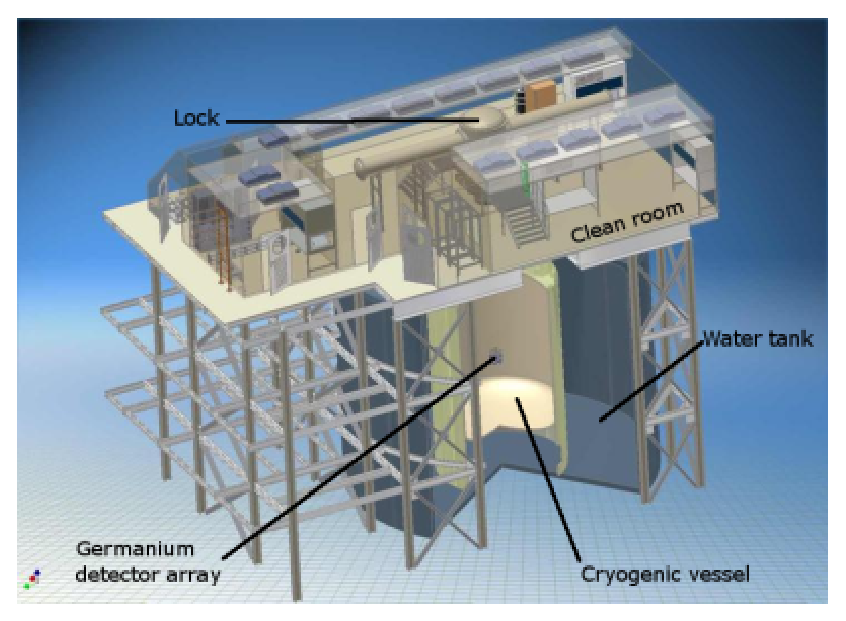
\includegraphics[width=0.7\textwidth]{gerda}  
  \caption{Structure of GERDA from engineer's view.}
  \label{fig:gerda}
\end{figure}

\subsection{Cosmic ray induced background}
\label{sec:gerda:loca}
In order to reduce the cosmic ray induced background GERDA was chosen to be located in Hall A of the INFN Gran Sasso National Laboratory (LNGS), Italy. LNGS is the largest underground facility in the world for low-background experiments. It can be accessed from a 10~km long highway tunnel under the Gran Sasso mountains. It has three experimental halls hosting a large variety of experiments, most of which focus on dark matter or neutrino physics. Fig.~\ref{fig:lngs} shows the location of GERDA in LNGS. The main experimental site of GERDA is between the Large Volume Detector (LVD) and a service tunnel across Hall A. The GERDA auxiliary and cryogenic storage system will be located in the service tunnel on the northeast side of Hall A.

\begin{figure}[tbhp]
  \centering
  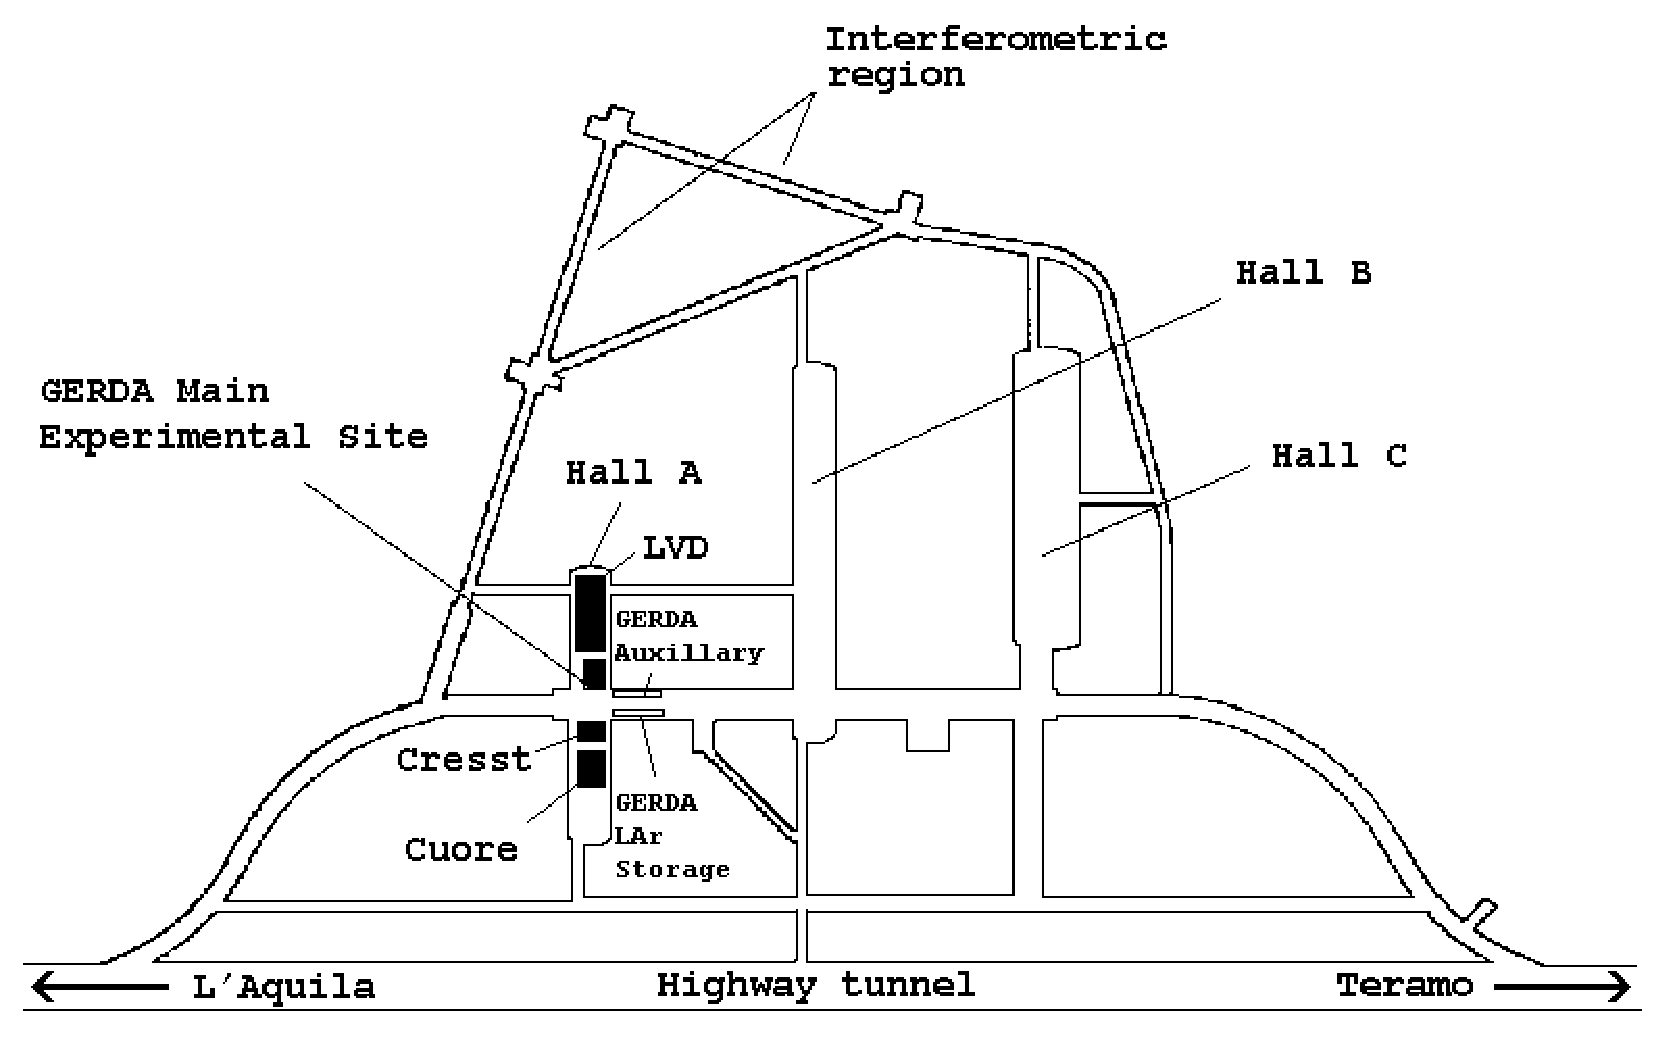
\includegraphics[width=0.8\textwidth]{lngs}  
  \caption{Location of GERDA in LNGS. The main experimental site of     GERDA is between the Large Volume Detector (LVD) and a service     tunnel across Hall A. The GERDA auxiliary and cryogenic storage     system will be located in the service tunnel on the northeast side     of Hall A.}
  \label{fig:lngs}
\end{figure}

The overburden of 1.4~km of rock on top of the experimental halls corresponds to 3.4~km meter of water equivalent (m.w.e). It reduces the cosmic ray induced muon flux by a factor of $10^{6}$, and neutron flux a factor of $10^{3}$ compared to the surface. The energy and angular distribution of cosmic ray muons in Hall A of LNGS have been precisely measured~\cite{Amb95, Lip91, Amb03}. A comprehensive study of cosmic ray induced muon and neutron background in underground laboratories can be found in Ref.~\cite{Mei06}.

In order to further reduce the muon induced background additional muon veto system will be implemented. Cosmic muons traversing the water buffer will cause Cherenkov radiation. To detect the radiation 66 photomultiplier tubes (PMTs) will be installed on the walls of the water tank. The positions of PMTs are optimized according to Monte Carlo simulation. Together with these PMTs the water tank could be operated as a Cherenkov detector. The detection efficiency is about 95\% depending on the incident angle of the muon. In order to compensate for the missing water volume around the neck of the cryostat plastic scintillator plates will be placed on top of the clean room. They are used to detect the muons entering the cryostat almost vertically. The combined detection efficiency is expected to be above 99\%.

\subsection{Background from rock}
\label{sec:gerda:rock}
To mediate and absorb the neutron radiation from the rock $\sim 630$~m$^{3}$ of ultra-pure water will be filled in a stainless steel tank with an outer diameter of 10~m and a height of about 8~m. Since liquid argon can be produced with a much greater purity than lead or even copper traditionally used for shielding, a total of approximately 98~t of liquid argon will be stored in a cryostat placed inside the water tank to shield $\gamma$-rays from the rock and water. The vessel is made of stainless steel with an internal copper liner. The height of the vessel is 5.88~m (7.62~m with the neck) while the outer diameter is 4.16~m.

\subsection{Background from detector suspension system and cables}
\label{sec:gerda:cable}
The detector array consists of hexagonally packed detectors with up to 5 layers. Up to 19 detectors can be placed per layer. The horizontal distance between the centers of two detectors is 9 cm. The vertical clearance between two detectors 3.3. TECHNICAL REALIZATION 25 is 5 cm. The array is divided into strings of vertically aligned detectors. Figure 3.3 (left) shows a seven string array of germanium detectors as designed for the Phase II of the GERDA experiment. The same figure (right) shows a top view of the full array indicat- ing the possible positions for the Phase I and Phase II detector strings as well as for the calibration sources.  The Phase I detectors are p-type diodes with a cylindrical closed-ended coaxial geom- etry. The detectors are enriched in 76Ge to a level of about 86% and have masses between 0.9 kg and 2.9 kg.  The detectors for Phase II will be cylindrical true coaxial n-type diodes. The precise size of the detectors will depend on manufacturing details. The most likely dimensions are a height of 70 mm and a diameter of 75 mm. The detectors will be segmented. The segmentation scheme under consideration is a 6-fold segmentation in the azimuthal an- gle φ and a 3-fold segmentation in the height z. Light-weight holders were designed for the Phase II detectors together with a novel contacting scheme. The holders are made out of approximately 30 g of copper. Figure 3.4 (left) shows a Phase II prototype detector mock-up with its cabling and holder structure.  Figure 3.3: Left: An array of 7 × 5 germanium detectors as described in the text. Right: Top view of the full array indicating the possible positions for the Phase I and Phase II detector strings as well as for the calibration sources.

\begin{figure}[tbhp]
  \centering
  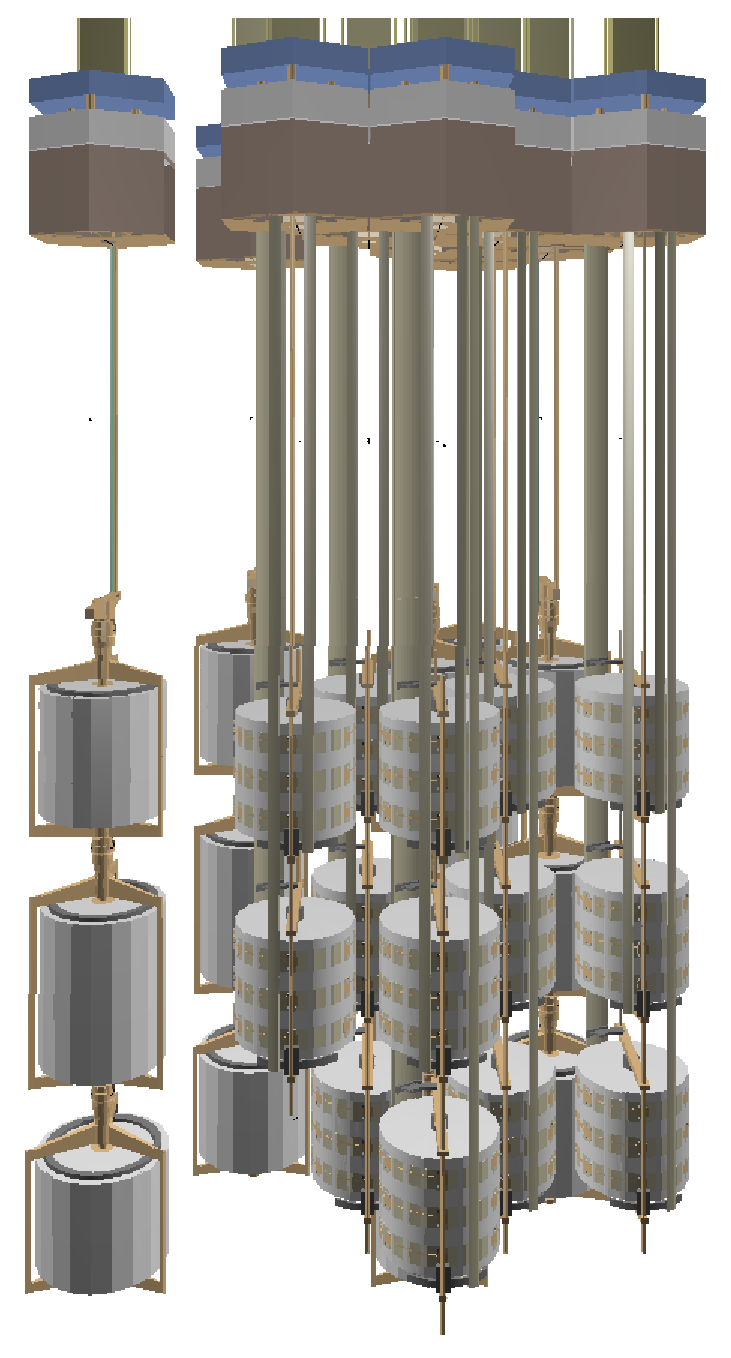
\includegraphics[width=0.25\textwidth]{array}\hfil
  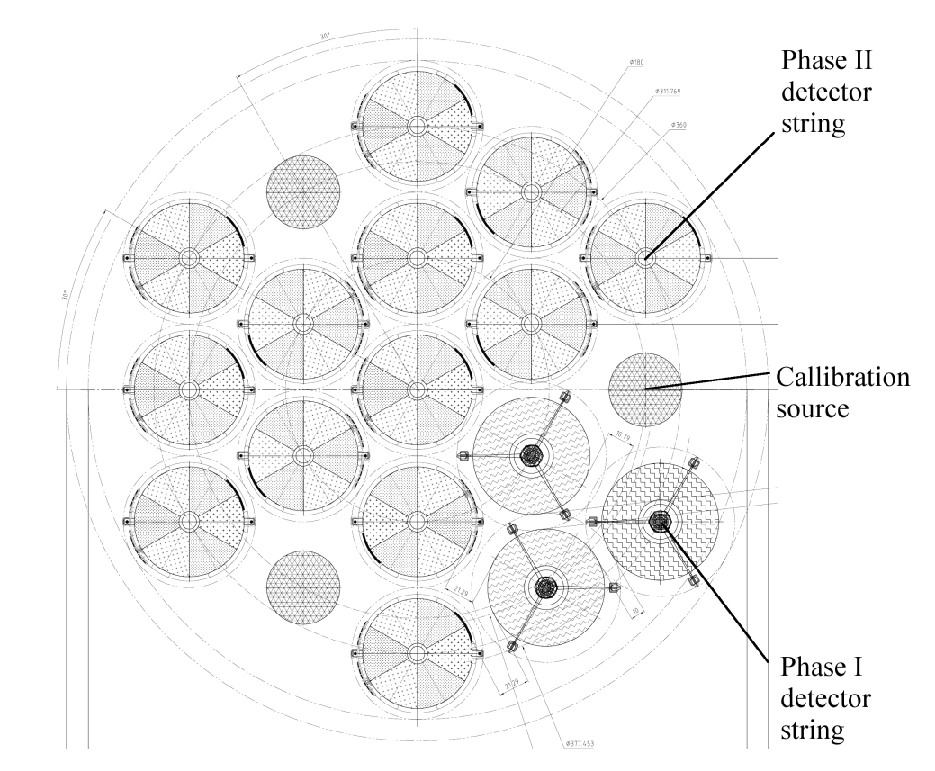
\includegraphics[width=0.6\textwidth]{arrayTop}  
  \caption{Detector array configuration.}
  \label{fig:array}
\end{figure}


\section{Background from detector}
\label{sec:gerda:source}

\section{Time, detector, segment anti-coincidence}
\label{sec:gerda:anti}
\section{Pulse shape analysis}
\label{sec:gerda:psa}

\section{Liquid argon scintillator}
\label{sec:gerda:scin}

The natural abundance of $^{76}$Ge (7.6\%) is
not very high, hence additional enrichment is needed.

\section{Sensitivity}
\label{sec:gerda:sens}

The physics goal is to
confirm or disprove the observation claimed by part of the HdM
Collaboration. 

Assuming an exposure of
100~(kg$\cdot$year), an upper limit on $m_{\beta\beta}$ of
0.09-0.29~eV would be achievable. 

 The sensitivity of $m_{\beta\beta}$ would be down to
0.05~eV.

%%% Local Variables:
%%% mode:latex
%%% TeX-master: "thesis"
%%% End:

\clearpage{\pagestyle{empty}\cleardoublepage}

\chapter{Signal formation in germanium detectors}
\label{cha:detector}
When particles, $\alpha, \beta, \gamma, n, p$, etc., interact with the germanium semiconductor detector, they will create electron-hole pairs, which are also called charge carriers. Driven by the external electric field applied to the detector, the charge carriers will drift, and induce electric signals in electrodes. The electric signals will be amplified, digitized and recorded by the electronics and data acquisition system connected to the germanium detector, and ready for the analysis. The whole process of the signal formation in the germanium detector and its surrounding electronics will be briefly reviewed in this chapter.

\section{Interactions of radiation with matter}
\label{sec:det:phys}

\section{Germanium semiconductor}
\label{sec:det:semi}

\section{Drift of charge carriers}
\label{sec:det:drift}

\section{Induction of signals in detector electrodes}
\label{sec:det:lamo}

\section{Effects of electronics on signal formation}
\label{sec:det:elec}

\section{Summary}
\label{sec:det:sum}



%%% Local Variables:
%%% mode:latex
%%% TeX-master: "thesis"
%%% End:

\clearpage{\pagestyle{empty}\cleardoublepage}

\chapter{Detector test facilities in Munich}
\label{cha:teststand}
Several test facilities at the Max-Planck-Institut f\"ur Physik, Munich, were founded for the research and development of segmented $n$-type germanium detectors for the Phase~II of the GERDA experiment. Based on them the operation and performance of several segmented detectors in vacuum as well as in cryogenic liquid have been systematically examined; various data samples have been taken to investigate the event discrimination power of segmented germanium detectors. A brief introduction of these test facilities is given in this chapter. The studies and analysis based on them are described in the following chapters.

\section{Phase~II prototype detectors} 
\label{sec:tt:dets} 
The first two prototype detectors for GERDA Phase~II have been developed and produced in close collaboration with the manufacturer Canberra-France, and called \emph{Siegfried} I and \emph{Siegfried} II. The \emph{Siegfried} series are $n$-type true coaxial cylindrical crystals made of natural germanium with a height of 70~mm and a diameter of 75~mm with a 10~mm hole in the center. The active volume is 302~cm$^{3}$, the total mass is 1.6~kg. They are 18-fold segmented with a 6-fold segmentation in the azimuthal angle $\phi$ and a 3-fold segmentation in the height $z$.  The segmentation scheme and the detector coordinate system are displayed in Fig.~\ref{fig:tt:segm} where a scheme of the cabling (left) and the segment numbering (right) are shown. The segments are read out using a Kapton flexible printed-circuit-board (FPCB) with snap-contacts~\cite{Sie07}. Pictures of the two detectors together with the contact cables are shown in Fig.~\ref{fig:tt:sies}. The detector specifications as provided by the
\mbox{manufacturer} are summarized in
Table~\ref{tab:tt:detpar}. 
\begin{figure}[tbhp]
  \centering
  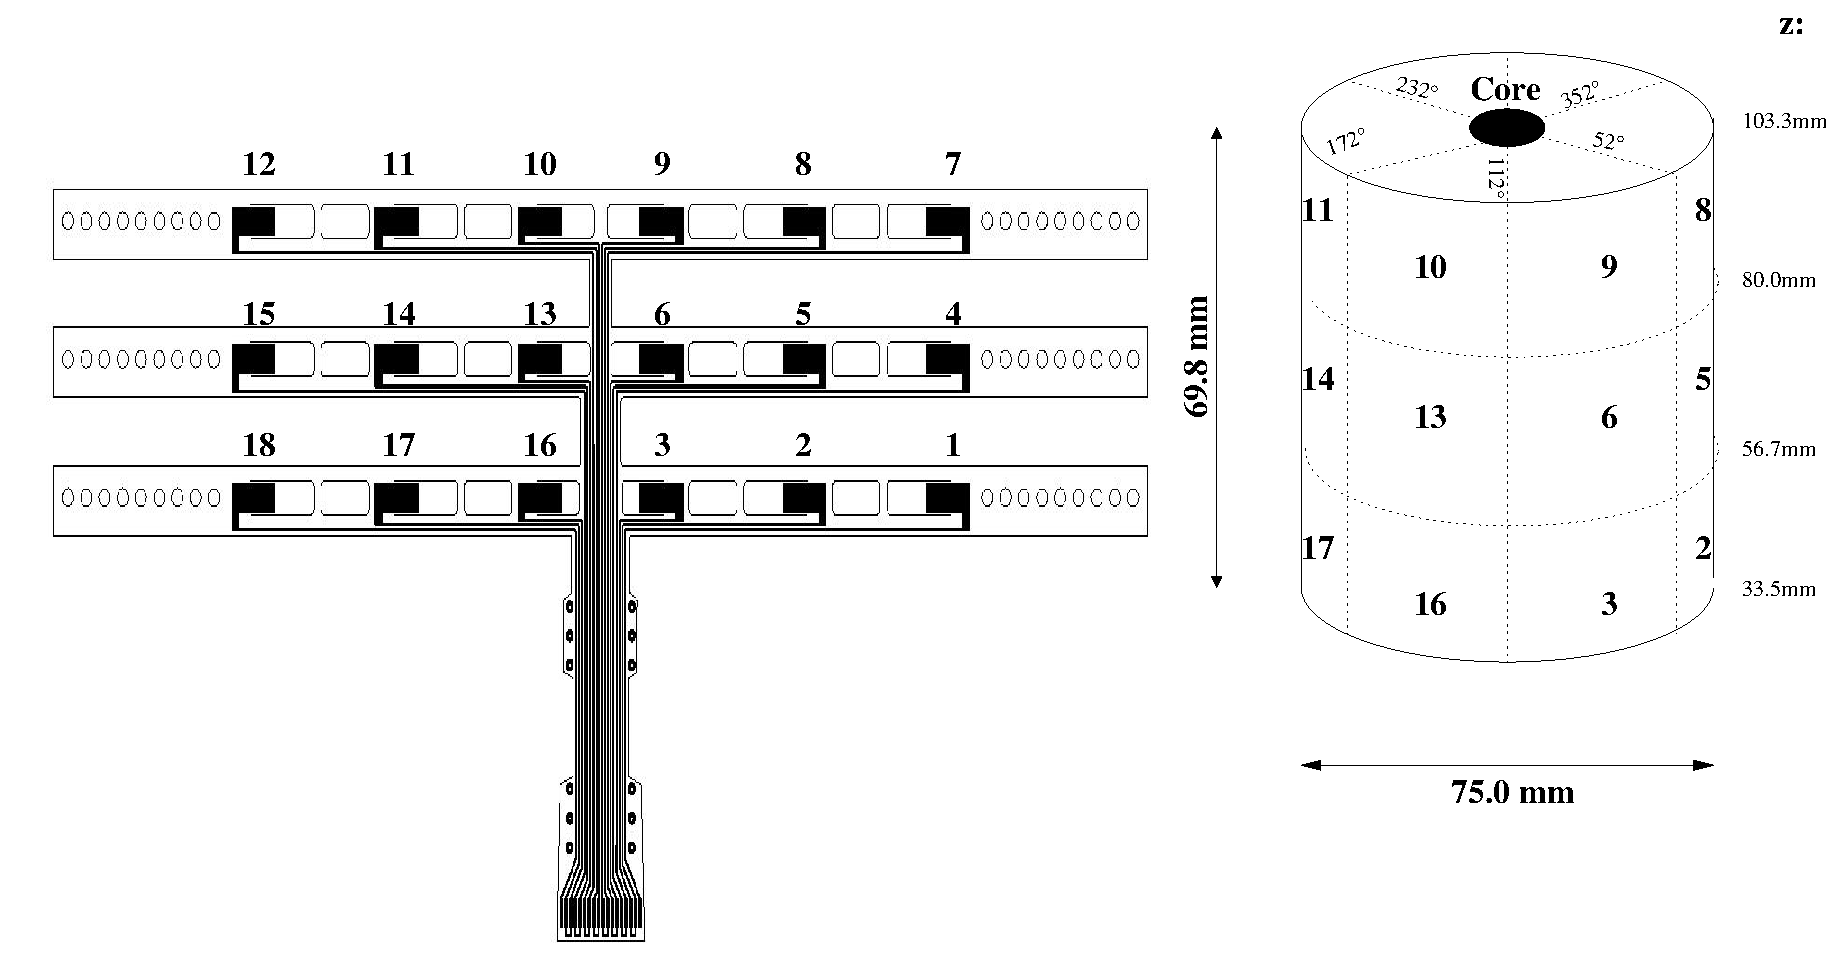
\includegraphics[width=0.95\textwidth]{segmentation_scheme}  
  \caption{Cabling scheme (left) and segment numbering (right) of the     prototype detector.}
  \label{fig:tt:segm}
\end{figure}

\begin{figure}[tbhp]
  \centering
  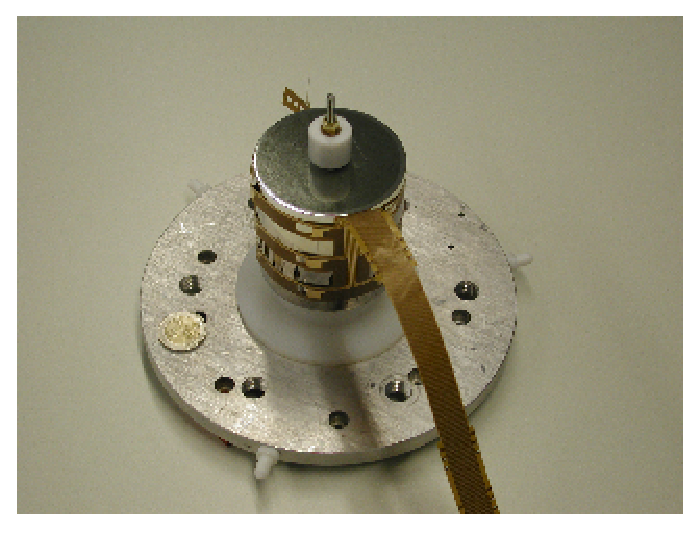
\includegraphics[height=0.25\textheight]{SiegfriedI}\hfil
  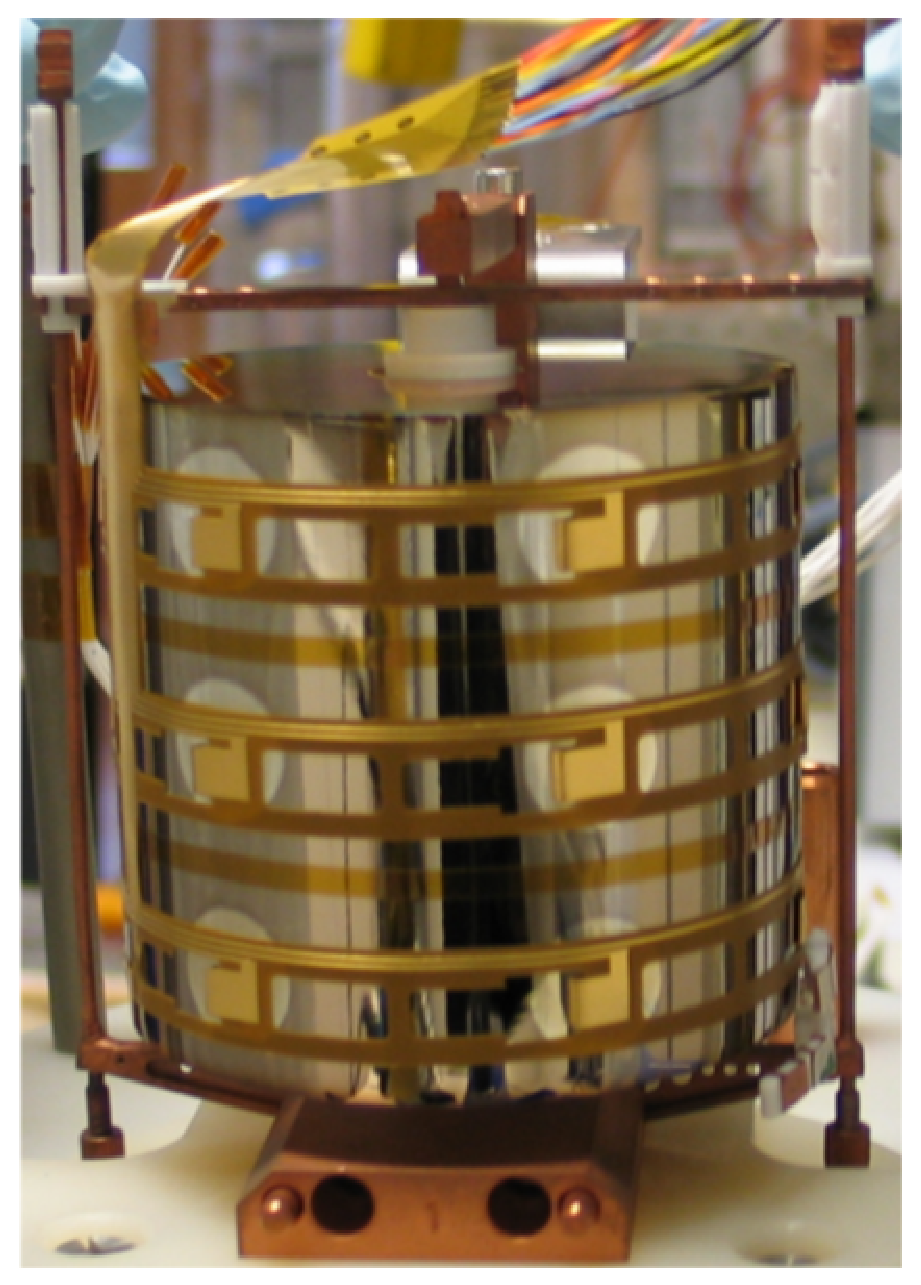
\includegraphics[height=0.25\textheight]{SiegfriedII}
\caption{Siegfried I mockup (left) and Siegfried II (right) with Kapton FPCB contact cables around.}
\label{fig:tt:sies}
\end{figure}

\begin{table}[tbhp]
\centering
\caption{Detector specifications as provided by the manufacturer.}
\label{tab:tt:detpar}
\begin{tabular}{lll}\\\hline
Parameter & \emph{Siegfried} I  & \emph{Siegfried} II \\\hline
Outer diameter (mm)   & 75.0 & 75.2\\ 
Inner diameter (mm)   & 10 & 10 \\ 
Height (mm)           & 69.8 & 70.2 \\\hline 
Operating voltage (V) & +3000 & +2000 \\ 
FWHM at 122~keV (keV)  & 0.99 & 0.96 \\ 
FWHM at 1333~keV (keV) & 1.99 & 2.11 \\ \hline 
\end{tabular}
\end{table}


\section{Cryostats}
\label{sec:tt:cryo}

\subsection{Commercial cryostat}
\label{sec:tt:comc}
\emph{Siegfried} I was delivered with a commercial cryostat as shown in the left picture of Fig.~\ref{fig:tt:comcryo}. It was placed inside a two-walled aluminum vacuum can with a combined thickness of 6~mm. The detector center is at $z=66$~mm and $r=0$~mm, the vacuum can extends up to $z=116$~mm and $r=75$~mm. A copper cooling finger was used as thermal link between the detector and a 60~l dewar below the detector filled will liquid nitrogen. A temperature monitor was used to measure the temperatures at several locations in the detector cryostat using Pt100 resistors. Liquid nitrogen was refilled daily resulting in a temperature stability of about $\pm3$~K. A comparison of spectra taken at different temperatures within this range showed neither significant differences in the general shape of the spectra nor in the energy resolution.

The core and each segment of \emph{Siegfried} I were read out through two massive copper tubes on both sides of the vacuum can housing front-end electronics as shown in the right picture of Fig.~\ref{fig:tt:comcryo}. The left side provided the feed-throughs for the high voltage and the signal lines for segments~10--18, the right side serviced the signal lines for segments~1-7 and housed a multi-purpose connector for the signal lines for segments~8--9 and a test-input for the core pre-amplifier.

\begin{figure}[tbhp]
  \centering
  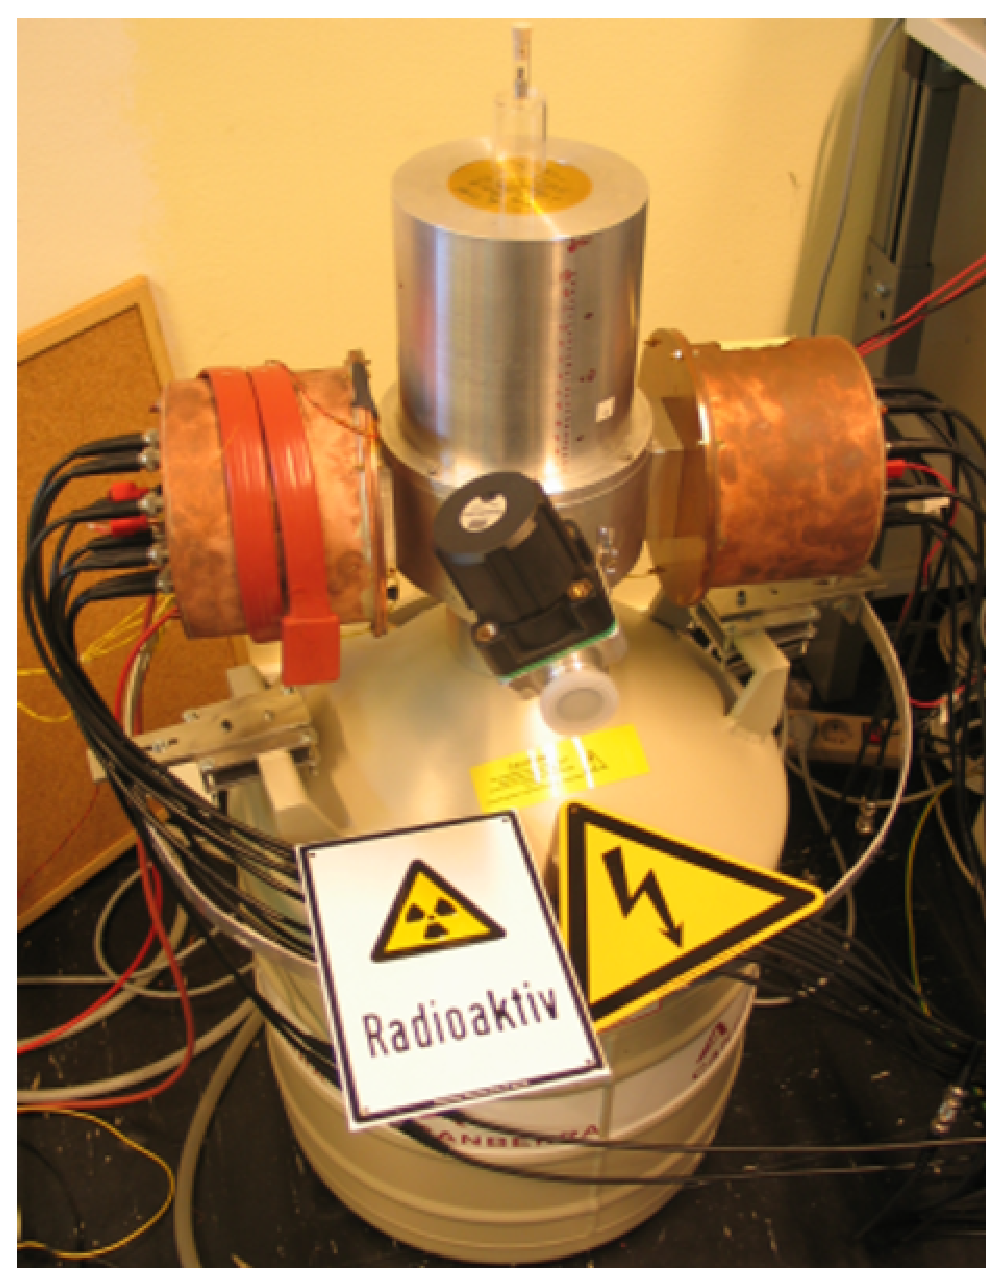
\includegraphics[height=0.25\textheight]{comcryo}\hfil
  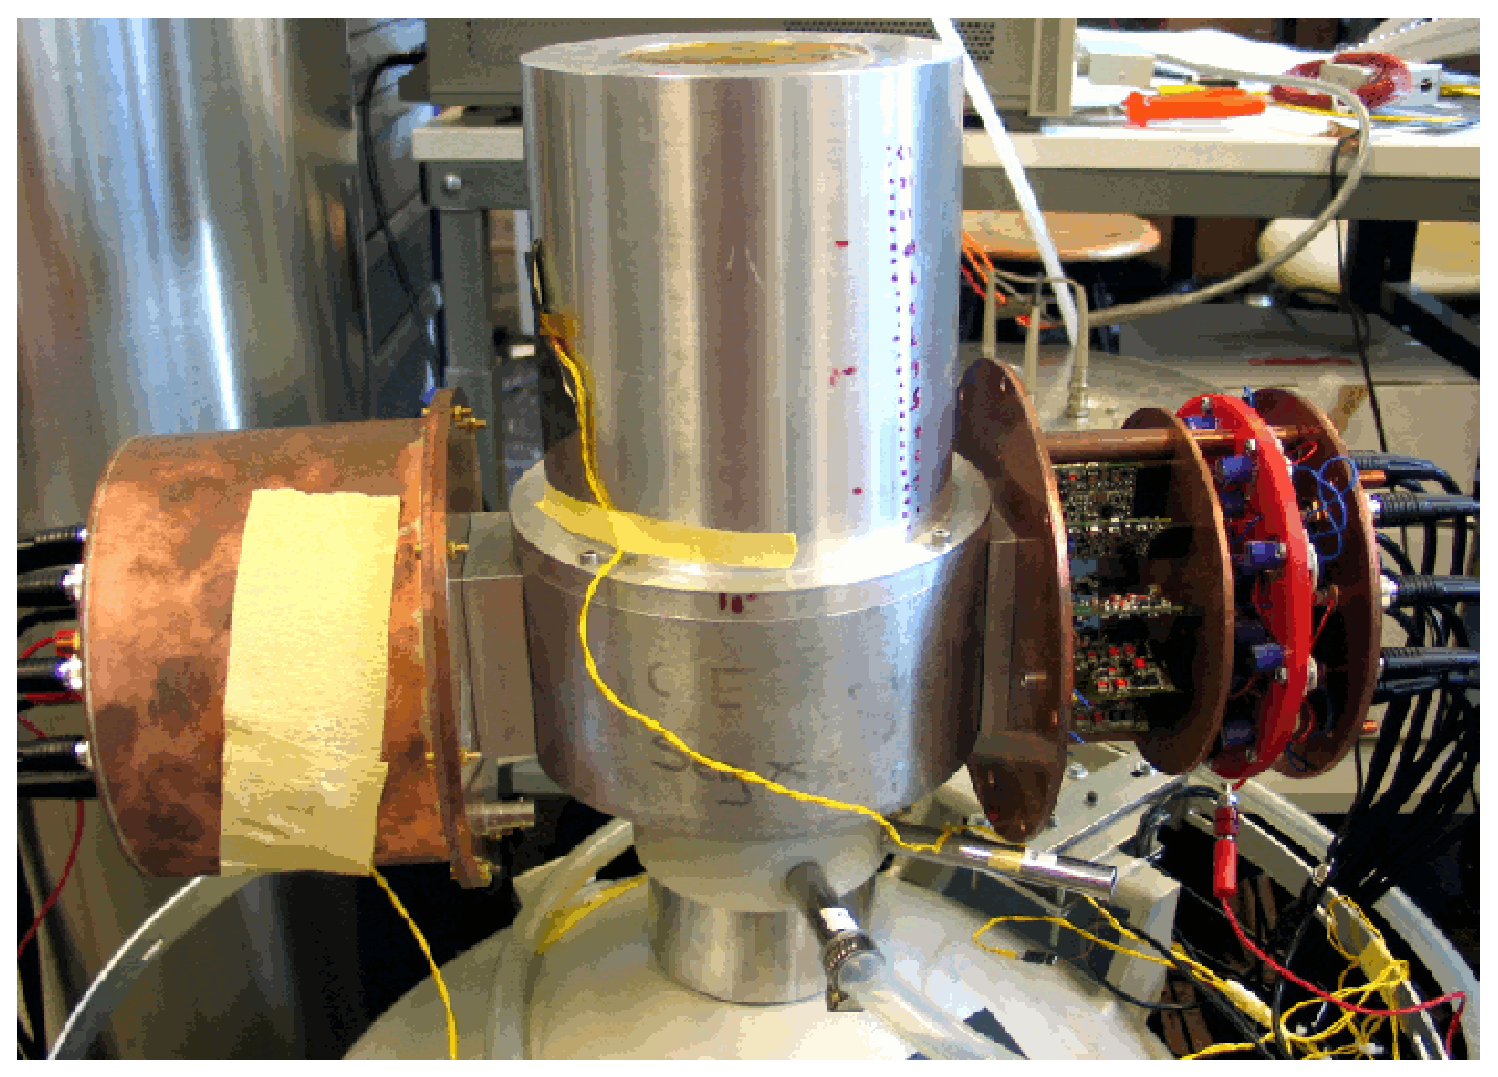
\includegraphics[height=0.25\textheight]{SIears}
  \caption{Left: commercial cryostat with \emph{Siegfried} I sitting     inside the top vacuum can. Right: a close-up to the vacuum can and     the copper ears housing pre-amplifier boards.}
  \label{fig:tt:comcryo}
\end{figure}

\subsection{Gerdalinchen II}
\label{sec:tt:gii}
Gerdalinchen II is a special cryostat manufactured in the technical division of Max-Planck-Institut f\"ur Physik for the test of operating several segmented germanium detectors directly in cryogenic liquid. As shown in the left drawing of Fig.~\ref{fig:tt:gii}, the main part of Gerdalinchen II is a two-walled cryogenic dewar sitting in a cylindrical aluminum tank with a hight of 960~mm and a diameter of 612~mm. The top flange can be lifted up vertically allowing mounting detectors to a vertical stainless steel bar under the flange and being lowered down into the dewar, as shown in the right picture of Fig.~\ref{fig:tt:gii}. The middle picture of Fig.~\ref{fig:tt:gii} shows the operation of a detector inside Gerdalinchen II with a neutron source placed aside. There are three high voltage feed-throughs and four signal connectors each with 18 channels on the top flange. This allows the operation of three 18-fold segmented detectors at the same time. The flange also contains tubes facilitating the re-filling of the dewar with cryogenic liquid, flashing with gaseous nitrogen and pumping without opening the system. The dewar is re-filled daily to prevent the cryogenic liquid level dropping down beneath the infrared shields (the thin copper tube and plate right above the detector as shown in Fig.~\ref{fig:tt:gii}). The liquid level is monitored by several thermal resistances (PT100) mounted in different places inside the dewar.

\begin{figure}[tbhp]
  \centering
  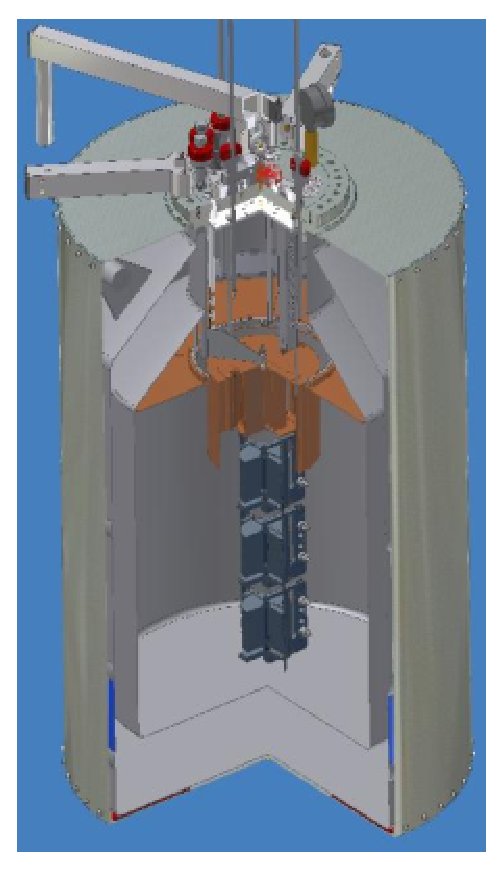
\includegraphics[height=0.25\textheight]{GIIdraw}\hfil
  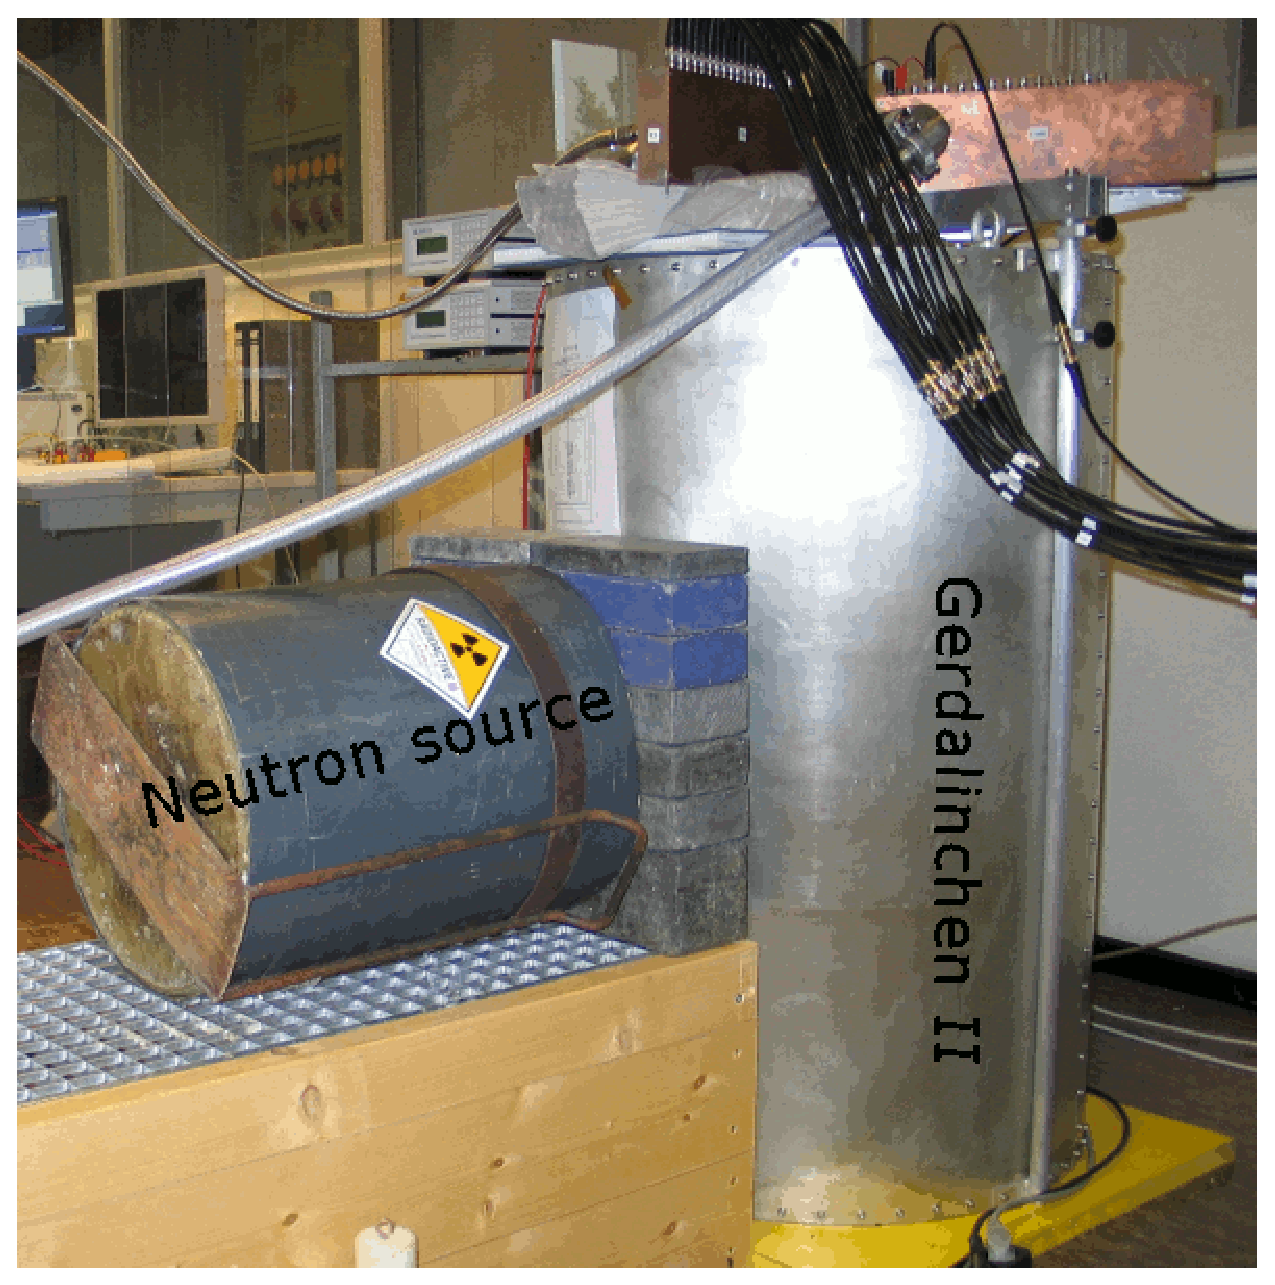
\includegraphics[height=0.25\textheight]{GIIneutron}\hfil
  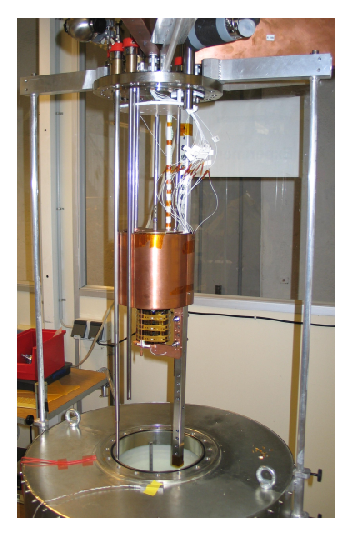
\includegraphics[height=0.25\textheight]{GIIdet}
  \caption{Left: technical drawing of Gerdalinchen II. Middle:     Gerdalinchen II in operation with a neutron source. Right:     Inserting a detector into Gerdalinchen II from the top.}
  \label{fig:tt:gii}
\end{figure}


\section{Electronics} 
\label{sec:tt:ele} 

\subsection{Front-end} 
\label{sec:tt:fend} 
A schematic diagram of \emph{Siegfried} I and its read out scheme are shown in the left plot of Fig.~\ref{fig:tt:sif}. The signals were read out using charge sensitive PSC-823C pre-amplifiers with a decay time of 50~$\mu$s. The FET for the core electrode was mounted inside the cryostat close to the detector, the FETs for the segment electrodes were incorporated into the pre-amplifier boards which were housed in the copper ears on both sides of the detector as shown in the right picture of Fig.~\ref{fig:tt:comcryo}. The right plot of Fig.~\ref{fig:tt:sif} shows the layout of the feed-throughs to \emph{Siegfried} I. They are placed on the end caps of the copper ears.

\begin{figure}[tbhp]
  \centering
  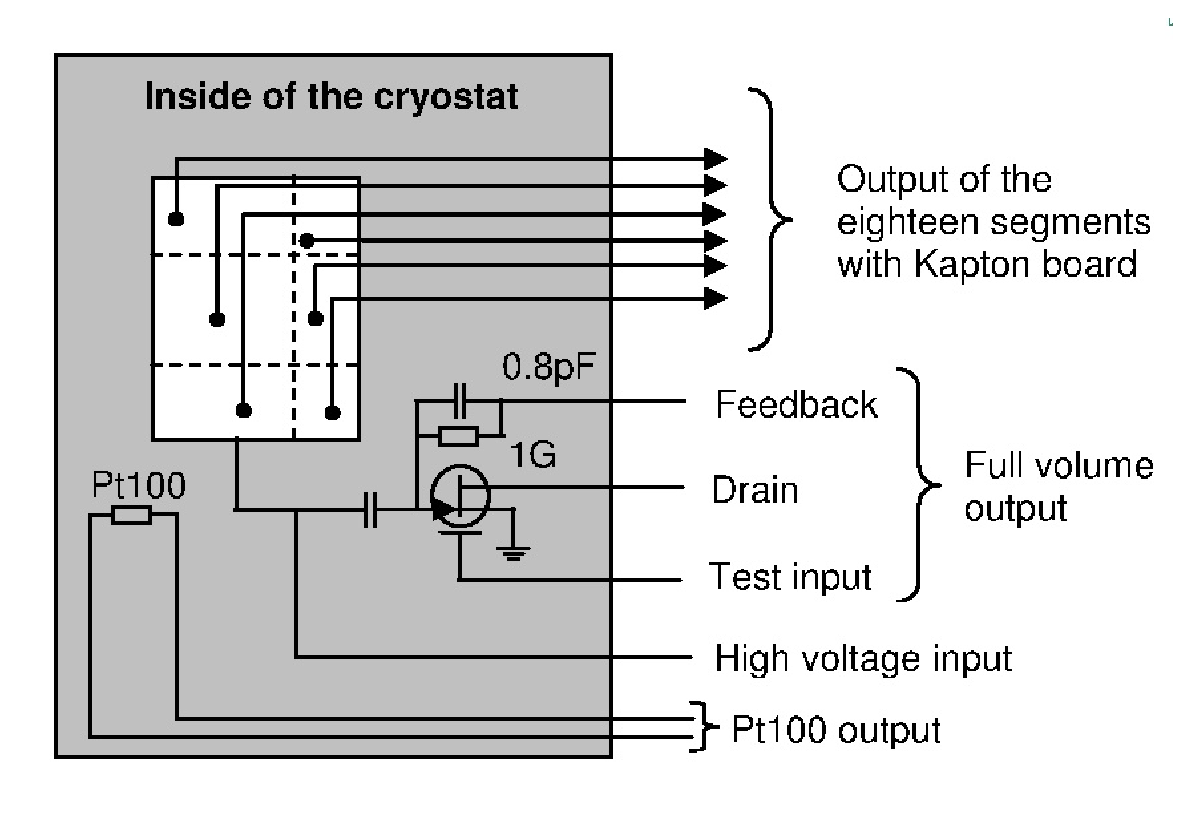
\includegraphics[height=0.25\textheight]{block1}\hfil
  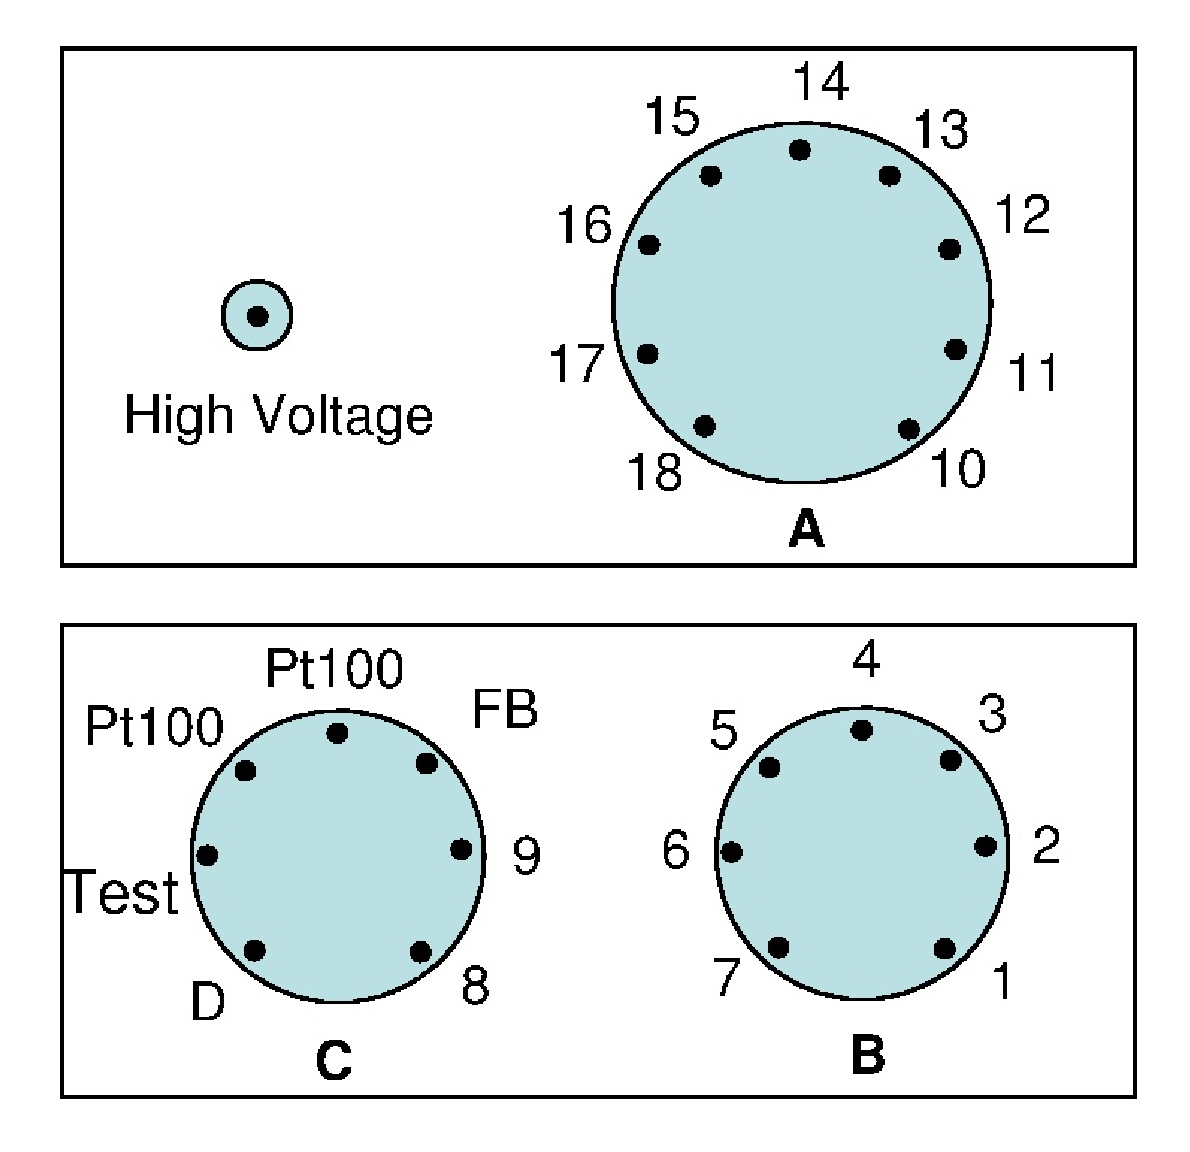
\includegraphics[height=0.25\textheight]{block2}
  \caption{Schematic diagram of \emph{Siegfried} I and its read out     scheme (left) and the layout of the feed-throughs to the     commercial cryostat (right).}
  \label{fig:tt:sif}
\end{figure}

For the operation of detectors in Gerdalinchen II a different setup was used. The FET for the core electrode was incorporated into the pre-amplifier boards like the segment electrodes. The core signal was not amplified before the pre-amplifier board, the cross talks to the segment signals from the core signal was minimized. All the pre-amplifier boards were mounted in a copper box and shared a common ground as shown in the right picture of Fig.~\ref{fig:tt:gef}. The noise filter for the high voltage lines and the coupling capacitors for the core signal cables were placed under the top flange as shown in the left picture of Fig.~\ref{fig:tt:gef}. They were operated above the cryogenic liquid level and moved later below the level for better temperature stability.
\begin{figure}[tbhp]
  \centering
  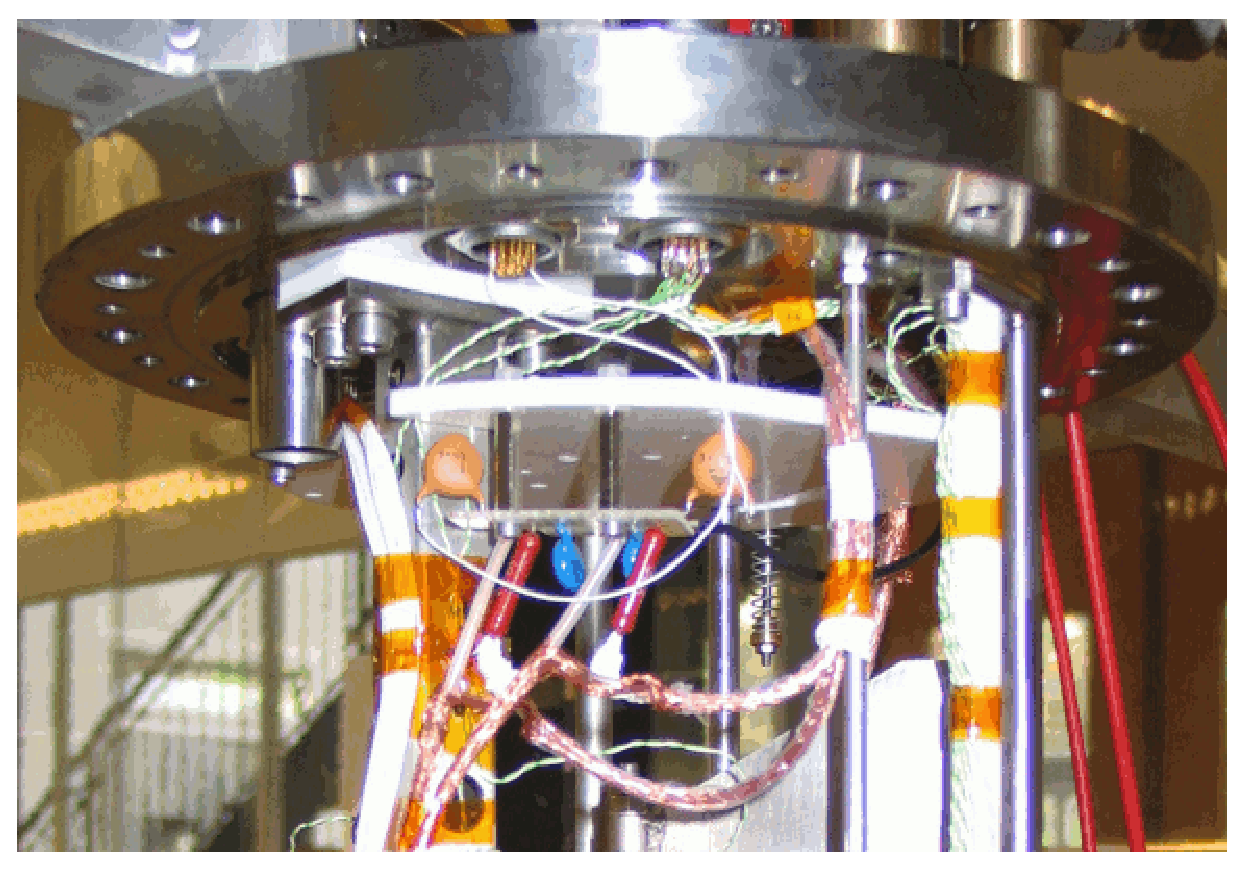
\includegraphics[height=0.2\textheight]{GIIHV}\hfil
  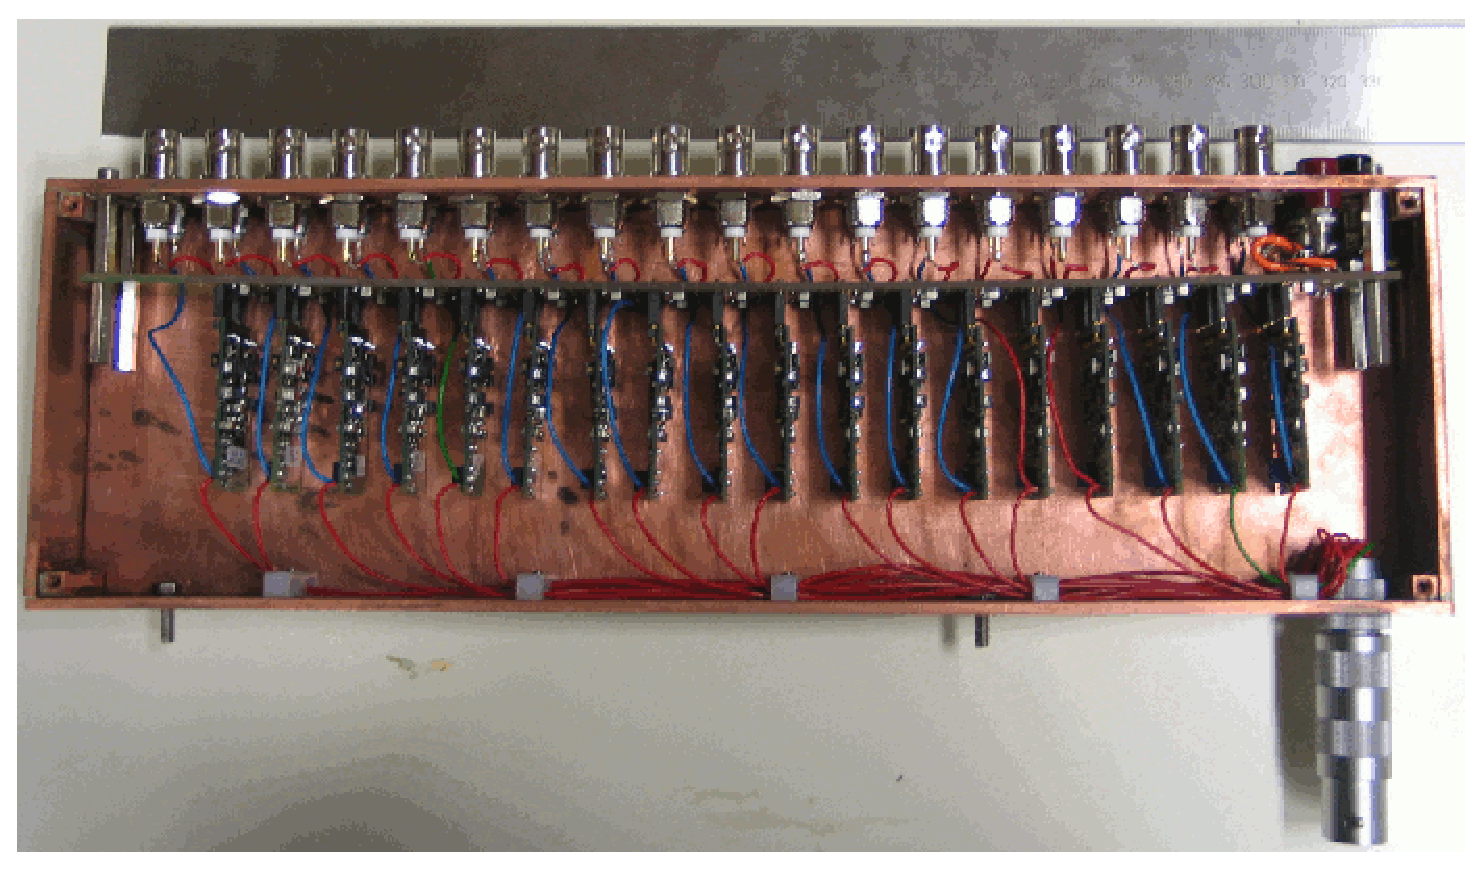
\includegraphics[height=0.2\textheight]{GIIpreamp}
  \caption{Left: high voltage filter and coupling capacitor in     Gerdalinchen II. Right: pre-amplifier box for one segmented     detector in Gerdalinchen II.}
  \label{fig:tt:gef}
\end{figure}

\subsection{DAQ} 
\label{sec:tt:daq}
The pre-amplified signals are digitized using a data acquisition system based on 5 14-bit ADC PIXIE-4 modules at a sampling rate of 75~MHz. The bandwidth of analog signals is limited by a Nyquist filter to half the sampling rate, \textit{i.e.} 37.5~MHz. This avoids aliasing in the noise from higher frequencies. It is implemented in the analog section of the PIXIE-4 module, with a low-pass Sallen-Key filter that makes a sharp (but finite) cut-off at this frequency. Energy is calculated using software filters~\cite{Pixie4}. Recorded pulse shape data consist of 300 samples of the integrated charge amplitude. The onset of the signal can be set by hand and was set to 1~$\mu$s for most of the measurements. The trigger and energy thresholds of the core and segment electrodes can be set to different values. The pile-up pulses can be rejected or recorded with a rough estimation of the energy.

\section{Accessories} 
\label{sec:tt:lamo}
The accessory equipments relevant to the operation of test facilities include high voltage supplies, temperature monitors, vacuum gauges, oxygen sensors, etc. Variables given by these equipments need to be monitored, recorded and analyzed in order to ensure a successful measurement. For overnight or long term measurements these monitoring processes need to be automated. A generalized Laboratory Monitor system, LaMo, has been developed to monitor and control most of the hardware in the laboratories using the graphic programming language, LabVIEW. The aim of the project is to create a slow control framework with a set of user friendly interfaces for most of the common lab tasks and to speed up the implementation of new pieces of hardware.

Fig.~\ref{fig:tt:lamo} shows the main panels of LaMo. The first panel one can see when opening LaMo is called ``laboratory'' as shown in the left screen shot of Fig.~\ref{fig:tt:lamo}. It shows a list of experiments going on in the laboratory and their status. An experiment can be created, edited, started, stopped using the bottoms aside the experiment list. The ``laboratory'' panel also provides functions common for all experiments, such as email alerts, power supply, oxygen sensors, etc. Different pieces of hardware relevant to an experiment can be chosen from a list of available hardware. This is done in the ``edit'' panel of LaMo as shown in the middle screen shot of Fig.~\ref{fig:tt:lamo}, where different hardware can be added, deleted from the equipment list for monitoring. Once an experiment is created and configured, it can be run by click the start bottom in ``laboratory'' panel. An ``experiment'' panel, as shown in the right screen shot of Fig.~\ref{fig:tt:lamo}, will be brought up, where monitored variables are shown in different ways. The functions specified for a particular experiment can be accessed from here.

\begin{figure}[tbhp]
  \centering
  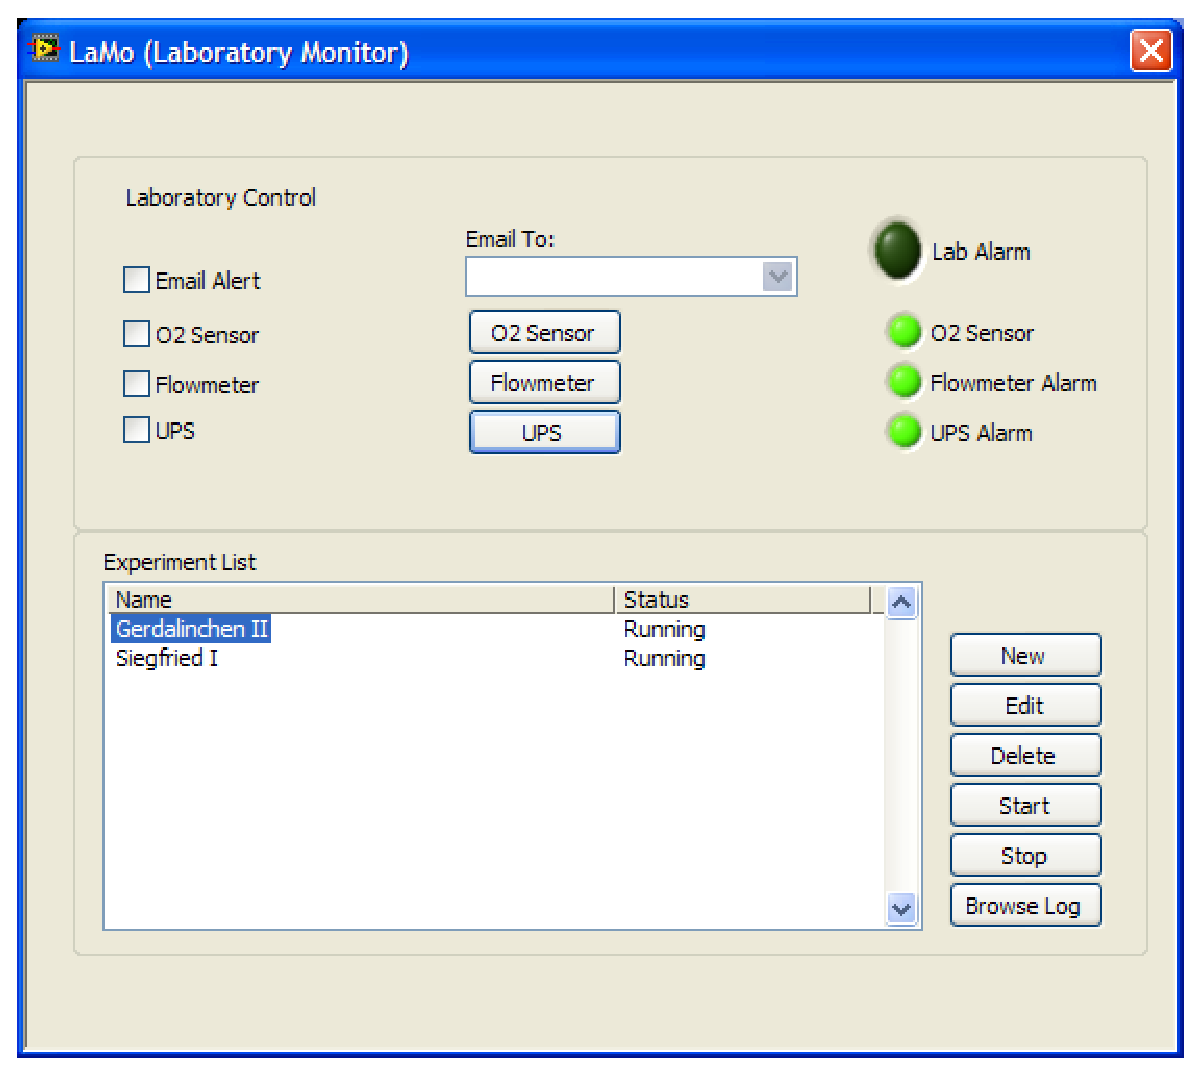
\includegraphics[height=0.23\textheight]{LaMoLab}\hfil
  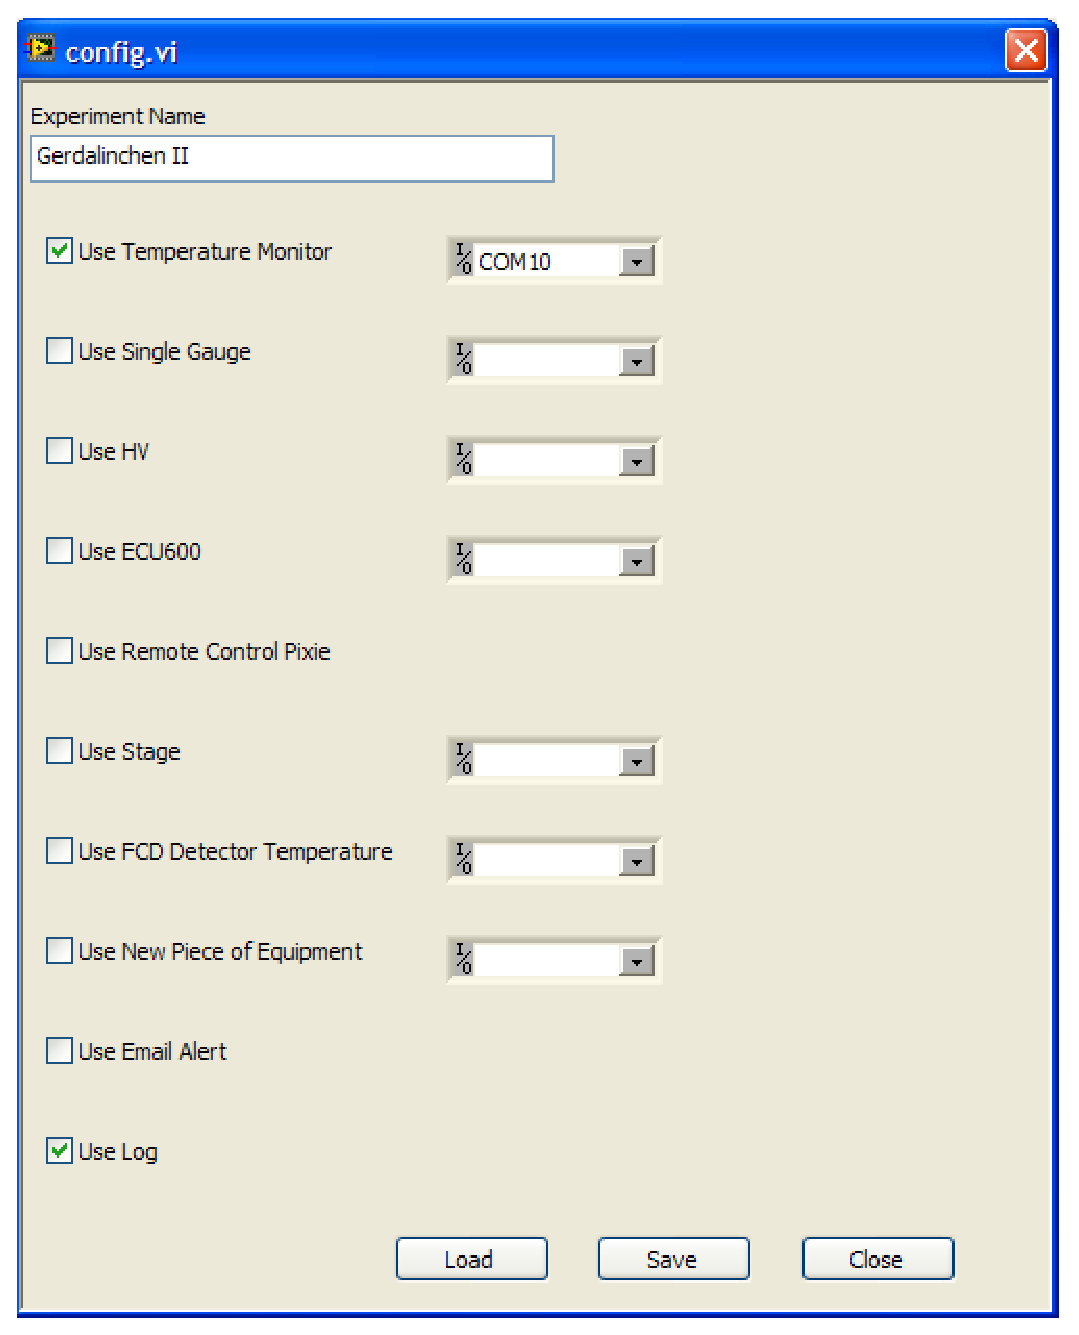
\includegraphics[height=0.23\textheight]{LaMoEdit}\hfil
  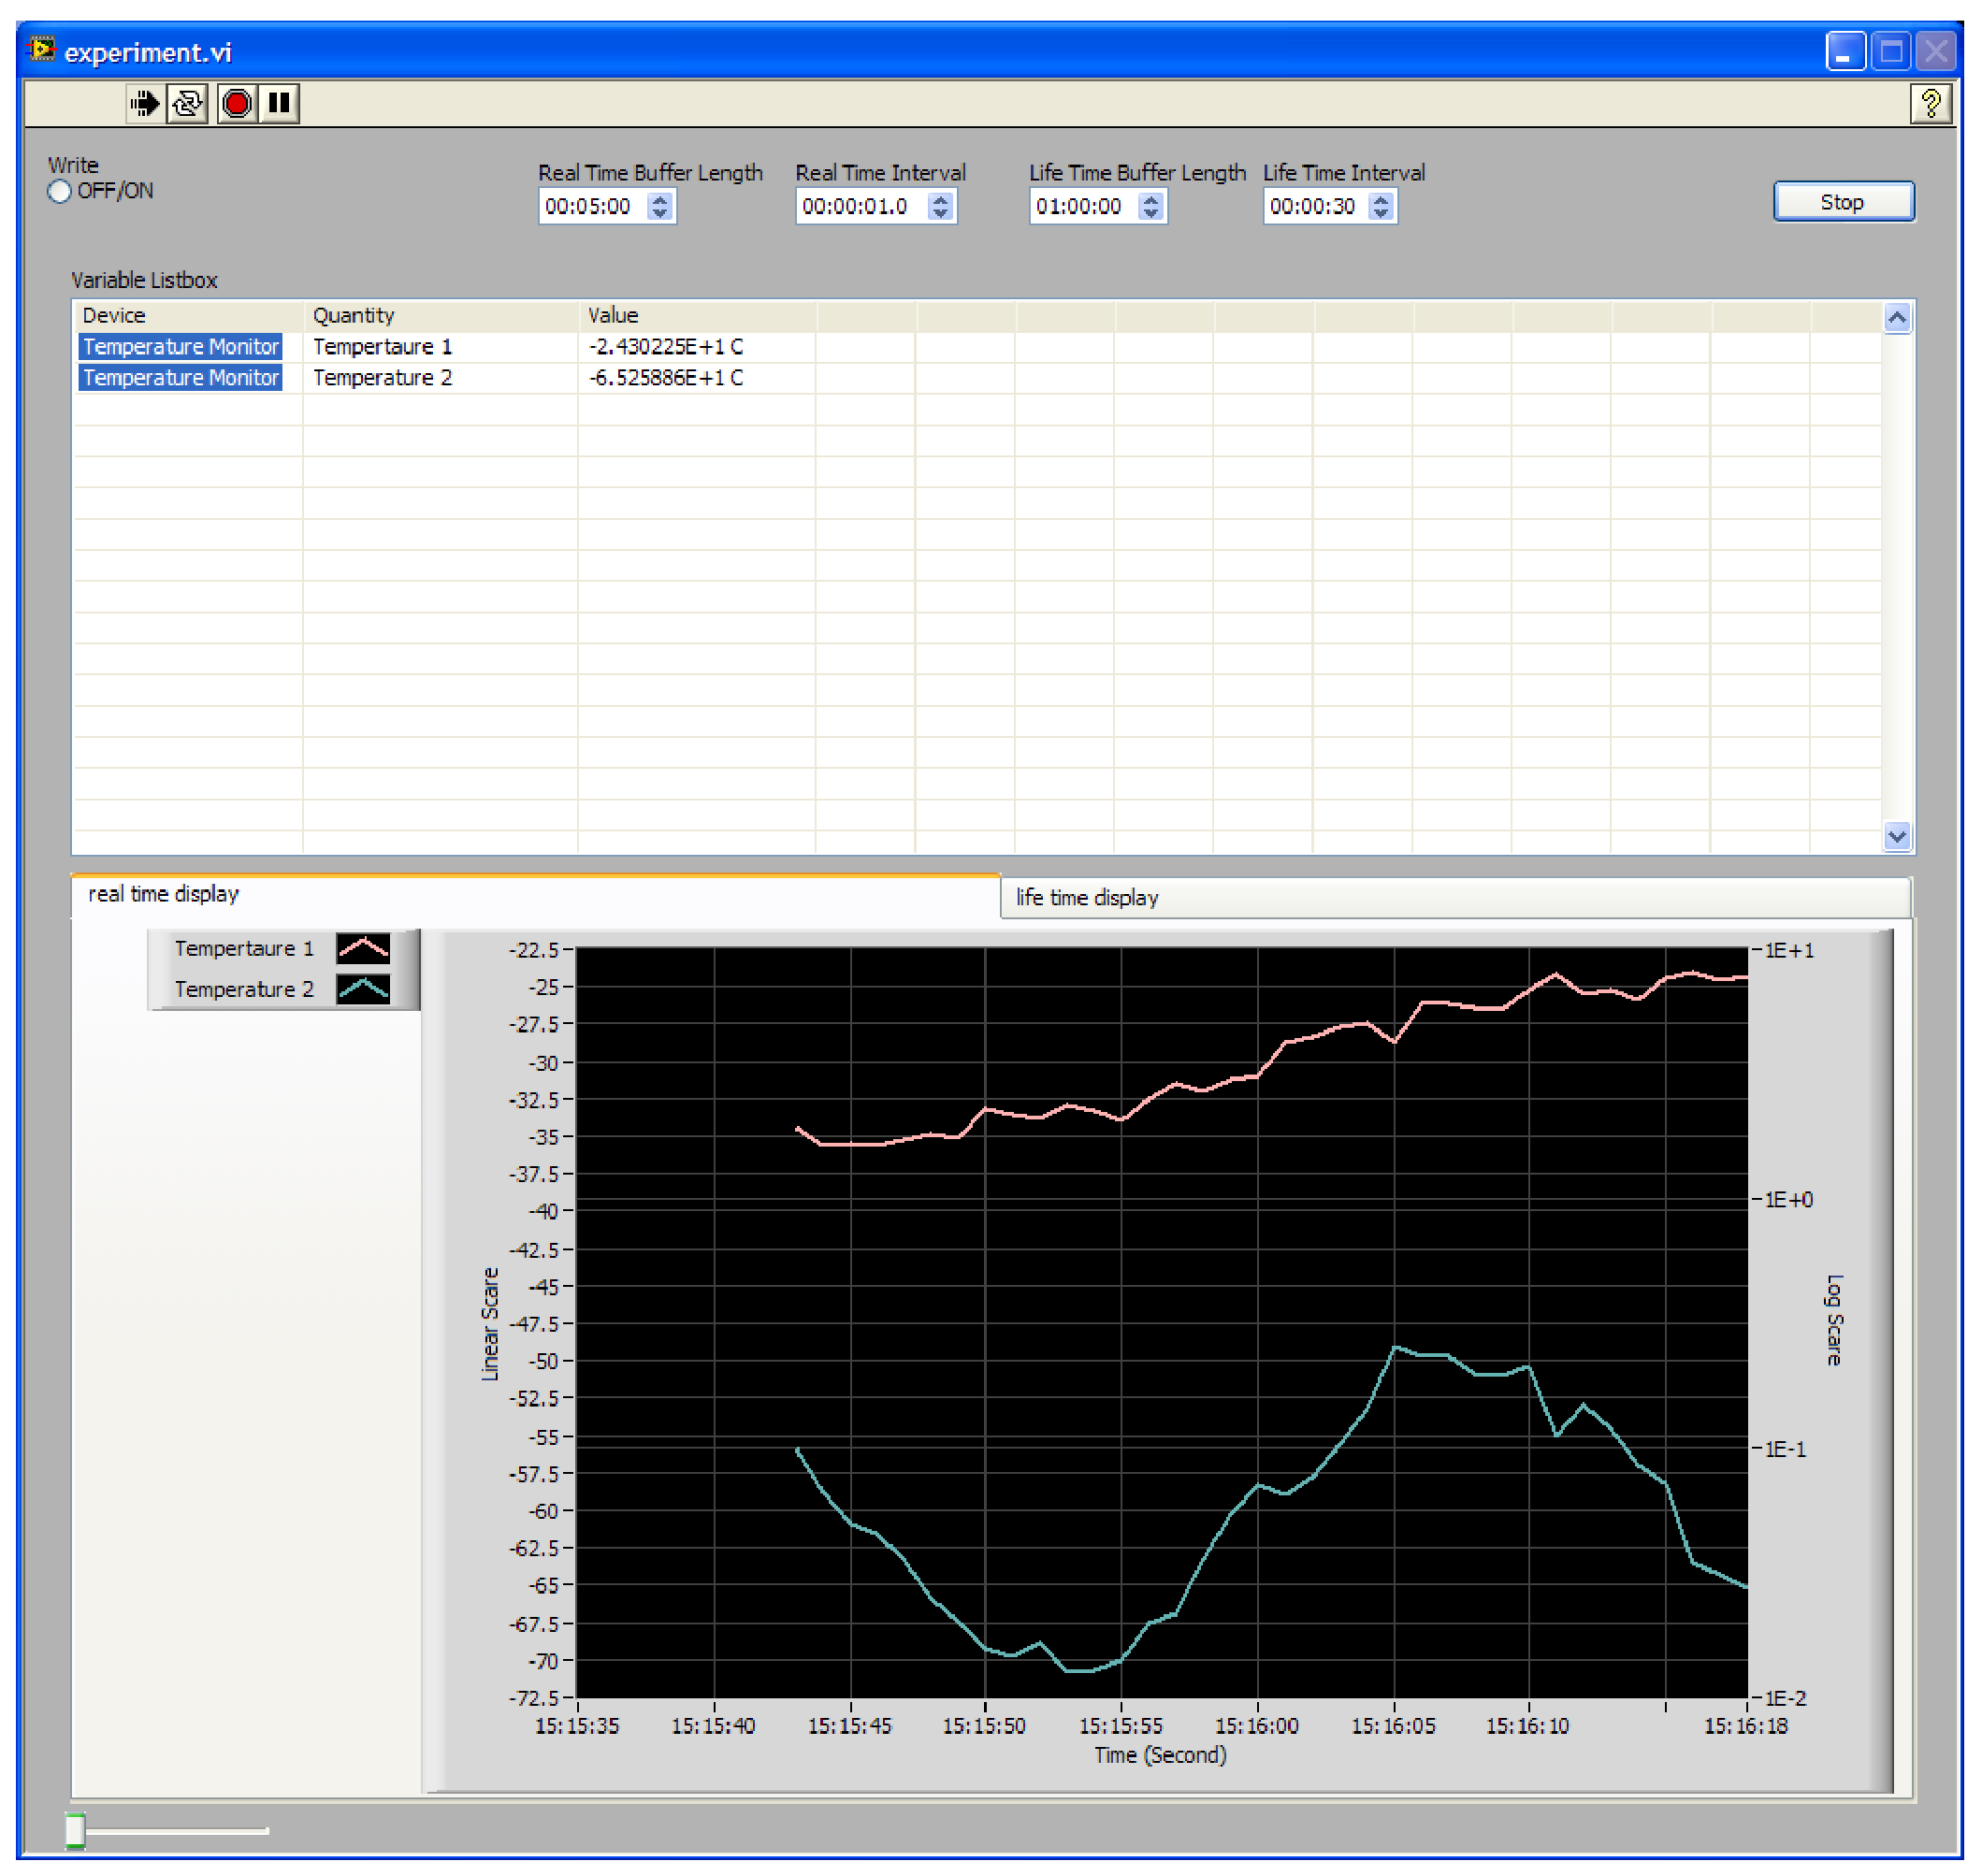
\includegraphics[height=0.23\textheight]{LaMoExp}
  \caption{Left: laboratory panel of LaMo, showing list of experiments     and their status, and giving access to functions common for all     experiments. Middle: edit panel of LaMo, where pieces of hardware     relevant to an experiment can be added/deleted from the equipment     list for monitoring. Right: experiment panel of LaMo, where     monitored variables can be shown in different ways. The functions     specified for a particular experiment can be accessed here.}
  \label{fig:tt:lamo}
\end{figure}

The common user interface enforces common I/Os for different pieces of hardware. The functionality of LaMo is modularized so that the effort to implement a new piece of hardware is minimized. To add a new equipment the developer only needs to define its I/O interface to LaMo. The other efforts, such as programming the user interface, etc., need not to be repeated every time.

\section{Monte Carlo simulation} 
\label{sec:tt:sim}
Monte Carlo simulations of prototype detectors and their cryostats was performed using MaGe~\cite{Mag08}, a C++ package co-developed by the Majorana and GERDA collaborations using Geant4 toolkits~\cite{Gea03,Gea06}. Figure~\ref{fig:tt:sim} shows the geometry models of the detectors and cryostats implemented in Geant4. The right plot of Fig~\ref{fig:tt:sim} shows a close-up of the \emph{Siegfried} II geometry. It was modeled in such a way that the details were implemented as close as possible to reality while the simulation efficiency did not decrease too much.

The energy depositions of hits in each segment were recorded and the core energy was calculated by adding all segment energies. The segment and core energies were individually smeared according to the energy resolutions of the detectors measured in the individual channels.

The spacial and time information of hits were also recorded, which served as parts of the input for the pulse shape simulation package. The geometry of detectors and the voltage bias applied were other input information for the pulse shape simulation. The detail of the pulse shape simulation is described in Chapter~\ref{cha:pss}.
 
\begin{figure}[tbhp]
  \centering
  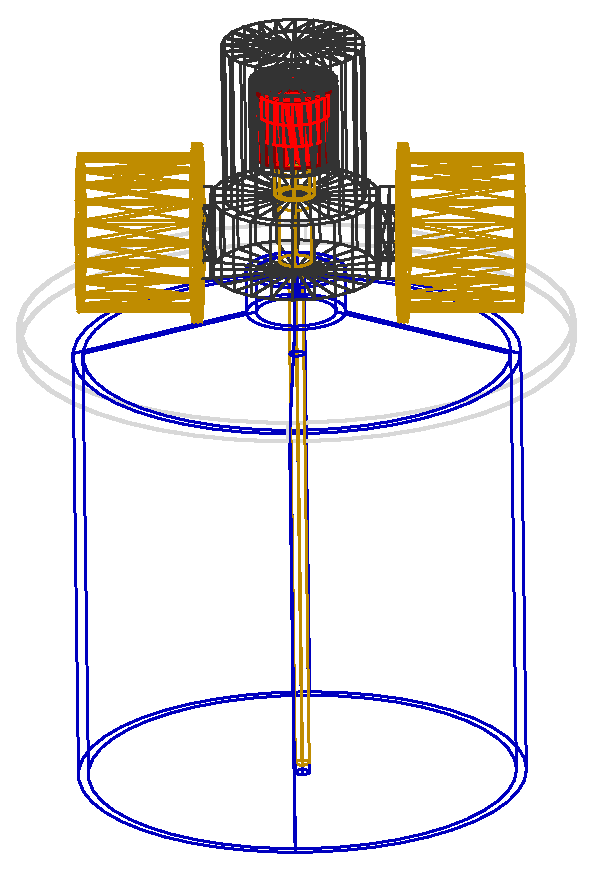
\includegraphics[height=0.3\textheight,clip]{SIwired}\hfil
  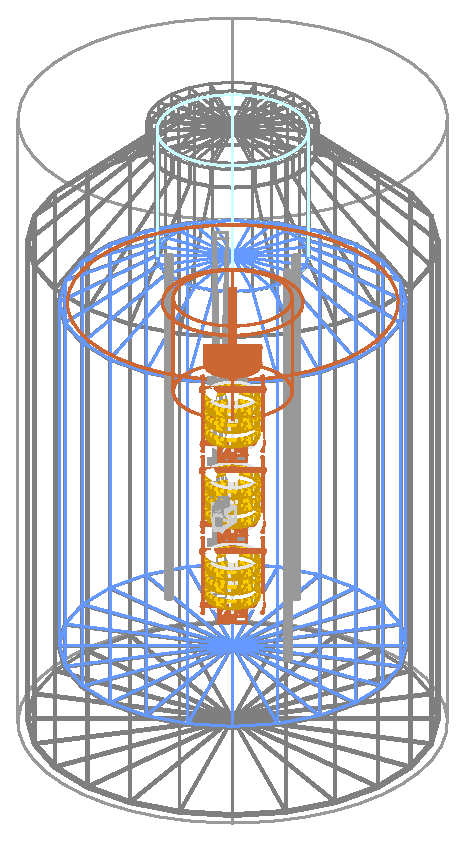
\includegraphics[height=0.3\textheight,clip]{GIIwired}\hfil
  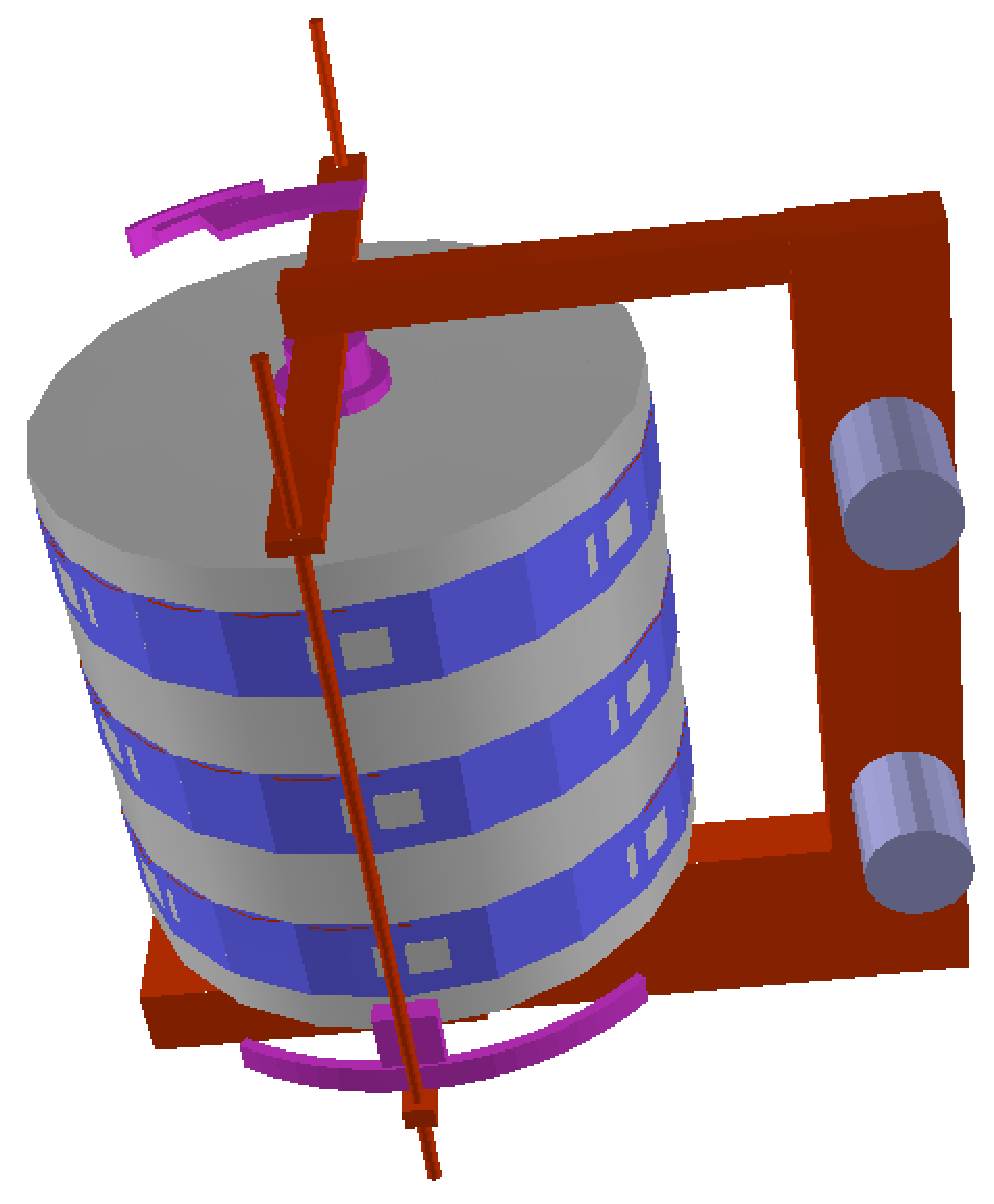
\includegraphics[height=0.3\textheight,clip]{SIIsolid}
  \caption{Left: wired drawing of the commercial cryostat geometry.     Middle: wired drawing of Gerdalinchen II geometry. Right: a     close-up of \emph{Siegfried} II geometry with copper supporting     frame as used in Gerdalinchen II.}
  \label{fig:tt:sim}
\end{figure}


%%% Local Variables:
%%% mode:latex
%%% TeX-master: "thesis"
%%% End:

\clearpage{\pagestyle{empty}\cleardoublepage}

\chapter{Operation of segmented detectors in liquid nitrogen}
\label{cha:GII}
\chapter[Operation of segmented detectors in LN$_{2}$]{Operation of segmented detectors in liquid nitrogen}
\label{cha:GII}
Segmented $n$-type germanium detectors will be directly submerged in cryogenic liquid in GERDA Phase II. It is therefore very important to study the performance of segmented detectors in cryogenic liquid. Siegfried~II,  the second 18-fold segmented $n$-type prototype detector built (see Sec.~\ref{sec:gerda:stat3}), was inserted into the Gerdanlinchen II test stand (see Sec.~\ref{sec:tt:gii}) containing liquid nitrogen on April 23rd, 2008. It was kept in liquid nitrogen for about 5 months and was warmed up on September 15th, 2008. The resolutions and leakage currents of the core and all segments were constantly monitored. Four short cool-down and warm-up cycles were carried out afterward to optimize the setup and perform dedicated measurements. The leakage currents were remeasured after each cool-down. The detector performance is summarized in this chapter.


\section{Experimental setup}
\label{sec:gii:setup}
The measurements were performed using the cryogenic test stand, Gerdalinchen~II (GII). A detailed description of GII can be found in Sec.~\ref{sec:tt:gii}. Figure~\ref{fig:ii:sch} depicts the test stand with three segmented detectors mounted inside. Only the upper and middle detector positions were occupied during the measurements. The dewar is filled bottom up through a filling tube. The numbers inside parentheses indicate the positions of eight PT100 thermal resistors. They were used to monitor the level of the liquid nitrogen. Liquid nitrogen was added once per day to keep its level between PT100 (2) and (3). This ensured that the infrared shields were always kept inside the liquid nitrogen minimizing the infrared radiation load on the detector. 

\begin{figure}[hbtp]
\centering
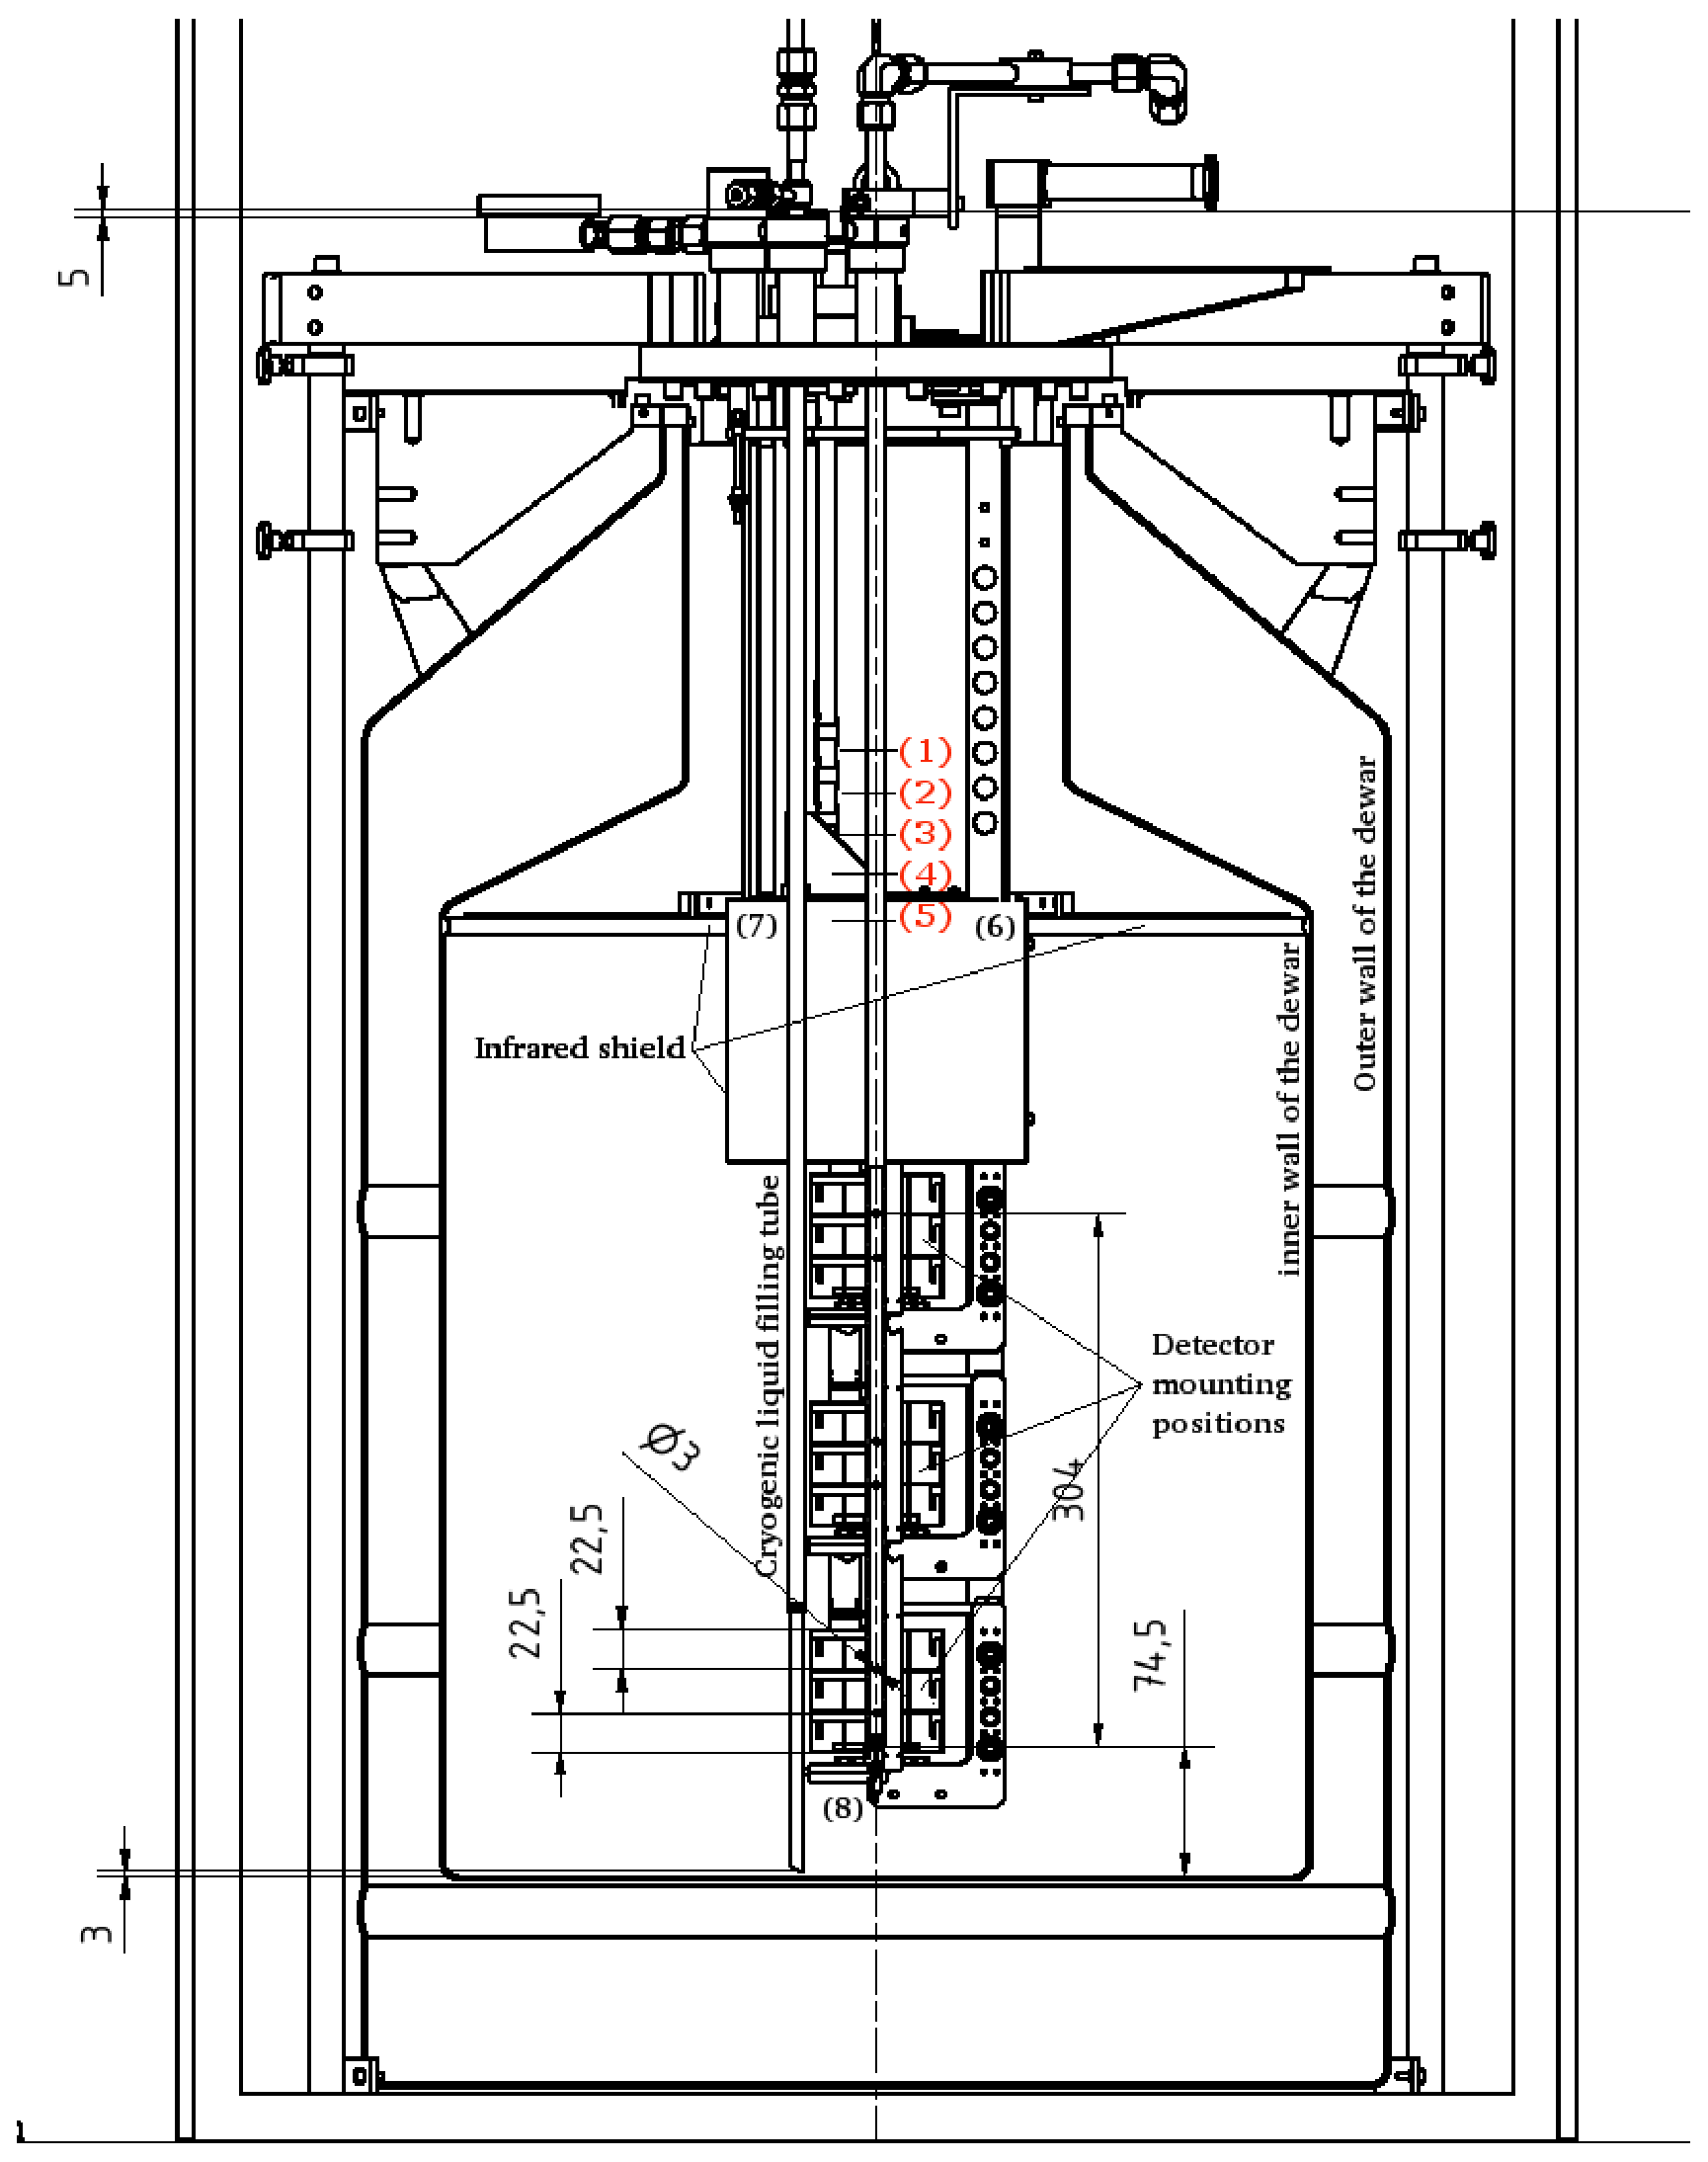
\includegraphics[width=\textwidth]{GIIscheme}
\caption{Gerdalinchen~II setup to operate segmented detectors in liquid nitrogen. For details see text.}
\label{fig:ii:sch}
\end{figure}

\section{Cool-down test}
\label{sec:ii:cool}
The speed, at which the detector strings will be lowered in GERDA, has to be chosen such, that the whole process can be finished in a reasonable time without subjecting the strings and detectors to dangerous thermal and mechanical stress. The submersion speed envisioned for GERDA is 10~mm/min. The temperature profile of a detector during the submersion process was studied in GII with an aluminum mock-up detector mounted at the highest GII position. 

The rising of the liquid nitrogen level was tuned to  about 10~mm/min. The temperature profile of the mock-up detector was monitored using three PT100 thermal resisters mounted on the top, bottom and in the middle of the mock-up. Figure~\ref{fig:ii:temp} shows the temperature profiles of the mock-up detector during the filling of GII. In addition it shows the temperatures measured by the thermal sensor 8 near the bottom of the dewar and the thermal sensor 1 at the top most position always above the liquid. The largest temperature difference between the top and bottom of the detector occurred at the first contact of the detector with the liquid nitrogen. It was about $130^{\circ}$C and lasted about three minutes. While germanium has a thermal conductivity four times smaller than aluminum at room temperatures, the thermal conductivities of germanium and aluminum are almost equal at 80\,K. Thus, it is expected that the germanium detector will cool down at about the same rate as the aluminum mock-up.

\begin{figure}[htbp]
\centering
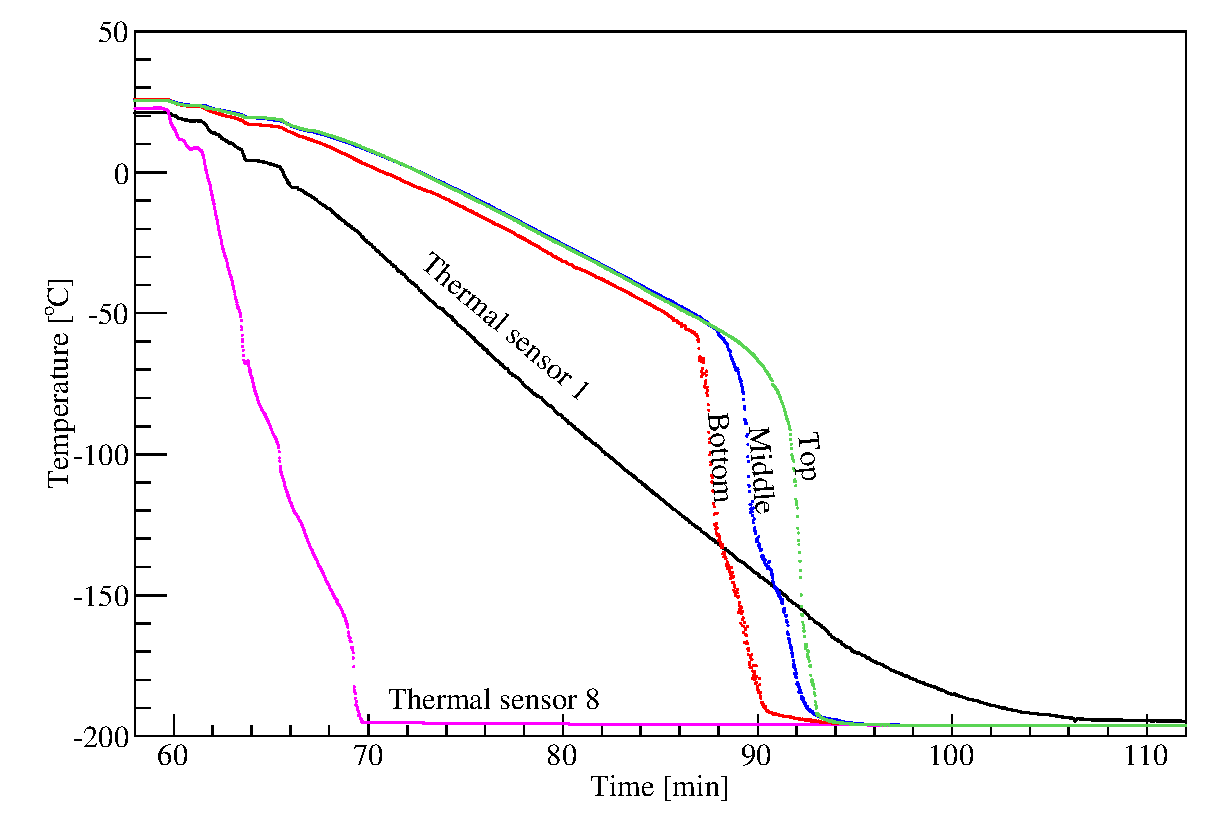
\includegraphics[width=0.8\textwidth]{temp}
\caption{Temperature profile of a mock-up detector during the cool-down process. Curves are shown for sensors mounted on top, middle and bottom of the detector. Also shown are curves for sensors 8 and 1 mounted close to the bottom and top of the dewar.}
\label{fig:ii:temp}
\end{figure}

\section{Resolution}
\label{sec:ii:sigma}
Siegfried II was mounted at the highest position in GII after a detailed cool-down procedure had been developed. It was cooled down on April 23$^{\text{rd}}$, 2008. The core and segment resolutions of Siegfried II were constantly monitored during the 140 days of operation. The variation of the resolutions (FWHM) at 1332~keV is shown for the core in Fig.~\ref{fig:ii:fwhm_core} and for all 18 segments in Fig.~\ref{fig:ii:fwhm_segs}.
\begin{figure}[hbtp]
\centering
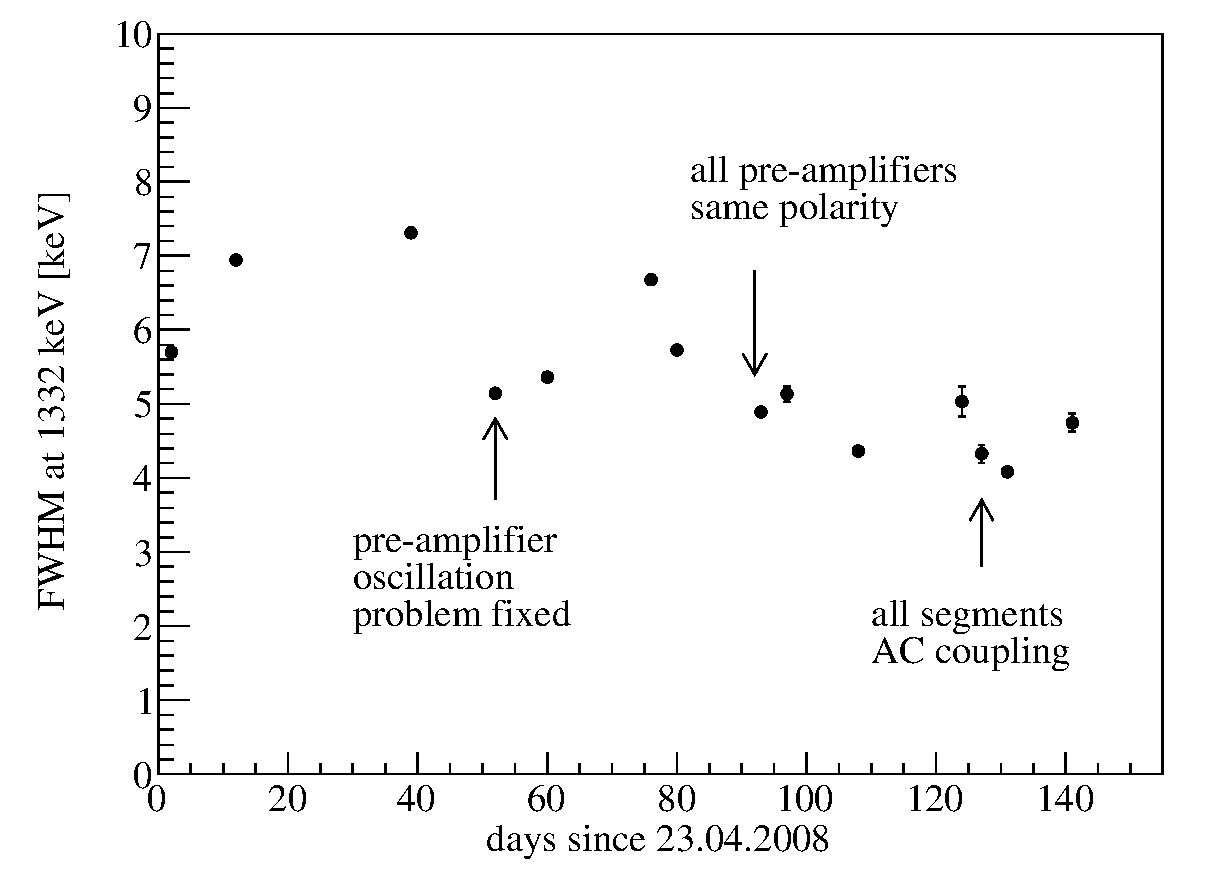
\includegraphics[width=0.6\textwidth]{fwhm_versus_time_core}
\caption{Core resolution of Siegfried II during 140 days of operation as determined from fits to the 1332~keV gamma line. The uncertainties on most values are hidden by the size of the dots.}
\label{fig:ii:fwhm_core}
\end{figure}

\begin{sidewaysfigure}[tphb]
\centering
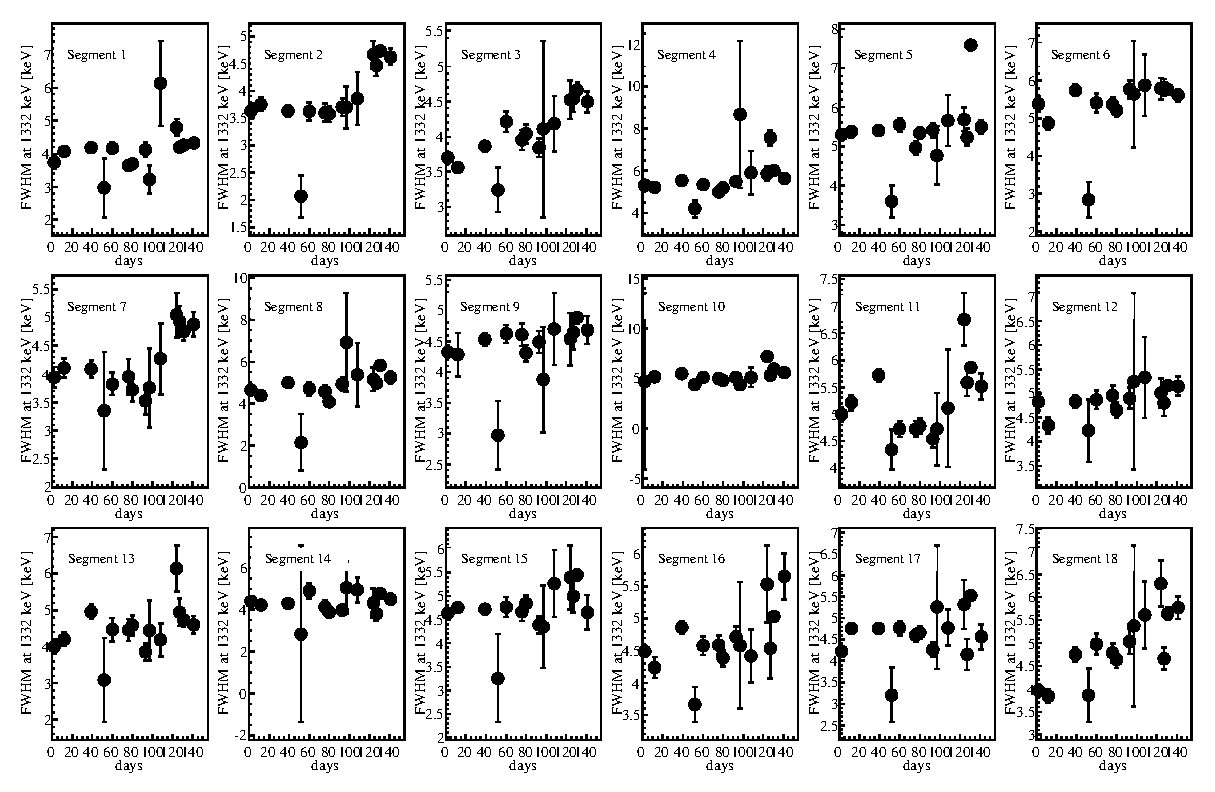
\includegraphics{fwhm_versus_time_segments}
\caption{Segment resolutions of Siegfried II during 140 days of operation as determined from fits to the 1332~keV gamma line.}
\label{fig:ii:fwhm_segs}
\end{sidewaysfigure}

During the first month of operation, all pre-amplifiers were oscillating whenever all 19 channels were read out simultaneously. The oscillations were due to an insufficient grounding scheme for the copper boxes holding and shielding the pre-amplifiers, see Fig.~\ref{fig:tt:gefb}. The problem was fixed by adding an extra copper plate inside the box, serving as the common ground for all pre-amplifiers. Afterward, all pre-amplifiers could be read out simultaneously and the core resolution was slightly better.

The second problem which affected the core resolution was related to the pulse polarity of the pre-amplifiers. Three pre-amplifiers (segments 3, 15 and 17) had a negative signal polarity while the rest had a positive one. This induced cross talk between these three pre-amplifiers and the core pre-amplifier. 
As a result the energy measured by the core for the 1332~keV photon line was 2~keV too low, if the energy was deposited in one of these three segments. These three pre-amplifiers were then replaced, resulting in some improvement in the core resolution as indicated in Fig.~\ref{fig:ii:fwhm_core}.

In order to decouple the segment potentials from the pre-amplifiers, all segment were AC instead of DC coupled ten days before the first warm-up, using 1~G$\Omega$ resistors and 2.2~nF capacitors. This neither influenced the core or segment resolutions.


\section{Leakage current}
\label{sec:ii:current}
The leakage current of Siegfried~II at 2000~V was monitored during the 140 days of operation. Two measurement methods were used: (a) a direct measurement using a picoameter and (b) an indirect measurement comparing the baselines at 0~V and 2000~V. The results from both methods are shown in Fig.~\ref{fig:ii:lc}. The leakage current stayed constant, around 20~pA.

\begin{figure}[htbp]
\centering
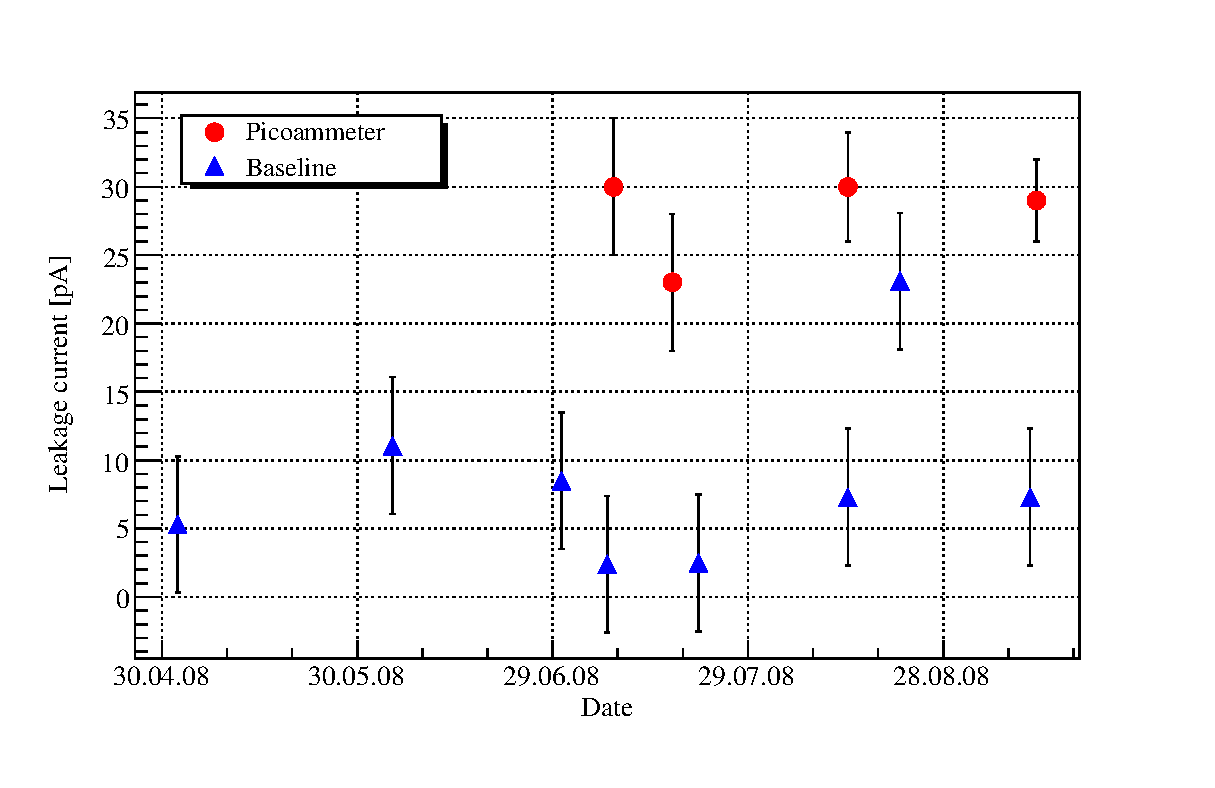
\includegraphics[width=0.6\textwidth, clip]{LC}
\caption{Leakage current of Siegfried II at 2000~V. The results from measurements using a picoameter(dots) and baseline shifts(triangles) are given.}
\label{fig:ii:lc}
\end{figure}

Siegfried~I was added to the setup  at the middle position in GII after the first warm-up of Siegfried~II. Afterward, four cool-down and warm-up cycles were performed. The leakage currents of both detectors at operational voltage after each cool-down are shown in Fig.~\ref{fig:ii:lcs1} and \ref{fig:ii:lcs2}, respectively. The current measured for Siegfried~I showed a significant increase after the third cool-down. This detector had previously been used to test HV contacts in the core and had to undergo reprocessing; it is known to have an imperfect core contact. The currents, measured for Siegfried~II immediately after each cool-down showed  dramatic increases. However, within 40~minutes they dropped back to their original value. Later investigation revealed an increasingly bad segment contact which could account for the effect.

\begin{figure}[htbp]
\centering
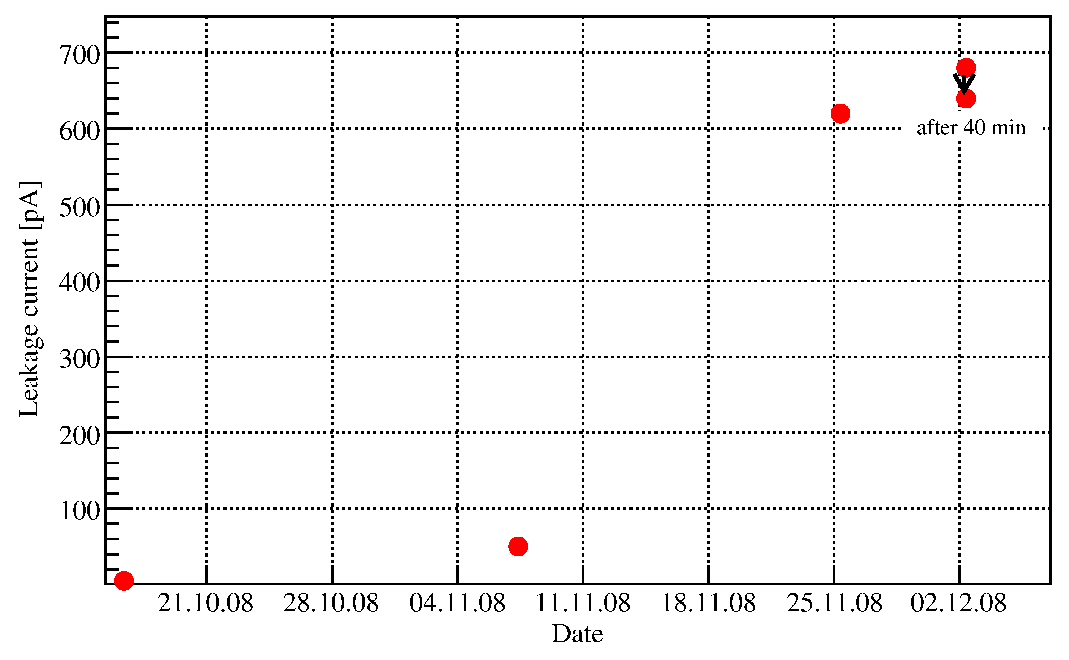
\includegraphics[width=0.6\textwidth]{LCs1}
\caption{Leakage current of Siegfried I at 3000~V right after each cool-down. The currents were measured using a picoameter.}
\label{fig:ii:lcs1}
\end{figure}

\begin{figure}[htbp]
\centering
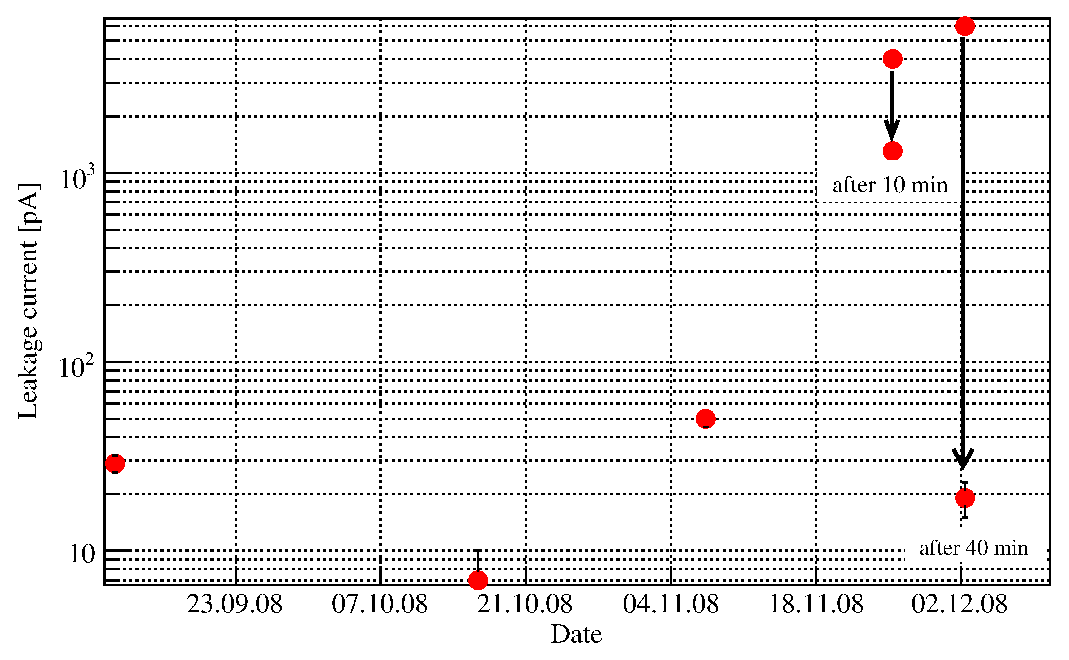
\includegraphics[width=0.6\textwidth, clip]{LCs2}
\caption{Leakage current of Siegfried II at 2000~V after each cool-down. The currents were measured using a picoameter.}
\label{fig:ii:lcs2}
\end{figure}

\section{Summary}
\label{sec:ii:sum}

The 18-fold segmented detector Siegfried~II was operated in liquid nitrogen for four months. No degradation of the performance was observed. Both the Siegfried~I and II detectors underwent four cooling cycles. It was observed that both the core and segment contacts are sensitive to the stress of such cycles. Especially the segment cables should be exchanged after multiple cool-downs.


%%% Local Variables:
%%% mode:latex
%%% TeX-master: "thesis"
%%% End:

\clearpage{\pagestyle{empty}\cleardoublepage}

\chapter{Photon induced background}
\label{cha:photon}
\chapter{Photon induced background}
\label{cha:photon}
Since the $0\nu\beta\beta$ decay of $^{76}$Ge has a $Q$-value of
2.039~MeV, $\gamma$-rays with energies larger than 2.039~MeV are the
main background source for GERDA. Fortunately, the spatial
distribution of photon interactions with germanium differs from
electron interactions with germanium, see
Sec.~\ref{sec:det:phys}. Segmented germanium detectors are considered
for use in GERDA Phase II in order to identify photon induced
background. The discrimination power of segmented germanium detectors
was examined systematically \cite{Pid07} using the GERDA Phase II
prototype detector Siegfried I (see Sec.~\ref{sec:gerda:stat3}) and
its test stand (see Sec.~\ref{sec:tt:comc}). The main results are
summarized in this chapter.

MaGe \cite{Mag06, Mag08} is a C++ simulation package co-developed by
the Majorana and GERDA collaborations based on Geant4 toolkits
\cite{Gea03, Gea06}. It was used for the simulation of GERDA and the
detector test facilities in Munich. The predictions for photon induced
events were verified to be accurate for a wide range of conditions.

\section{Event classification}
\label{sec:ph:eve}
As described in Sec.~\ref{sec:det:gamma} a photon with an energy of
the order of one MeV has a mean free path of several centimeters in a
germanium crystal. It most probably deposits energy in several
different places and creates a \emph{multi-site event}. On the other
hand, the average range of a 1~MeV electron in germanium is about
0.5~mm (see Sec.~\ref{sec:det:ep}). Since the probability for
Bremsstrahlung is low, electrons mainly create \emph{single-site
events} with most of the energy deposited within a radius of 1~mm. The
size of the segments was chosen such that electrons predominantly
create \emph{single-segment events} while photons result in
\emph{multi-segment events}.

Figure~\ref{fig:ph:eve} depicts four possible event configurations. By
requiring anti-coincidence most of the photon induced background
events can be rejected. However, there are still some photon induced
multi-site events with energy deposits in one segment only, as shown
in bottom left corner of Fig.~\ref{fig:ph:eve}. This kind of event can
be further identified using pulse shape analysis.

A single-site event can also be a multi-segment event if it happens to
occur on the boundary of two neighboring segments and induces signals
in both segments, as shown in the top right corner of
Fig.~\ref{fig:ph:eve}. This kind of event will be rejected erroneously
by the anti-coincidence requirement, and should also be identified
using pulse shape analysis.

\begin{figure}[htbp]
\centering
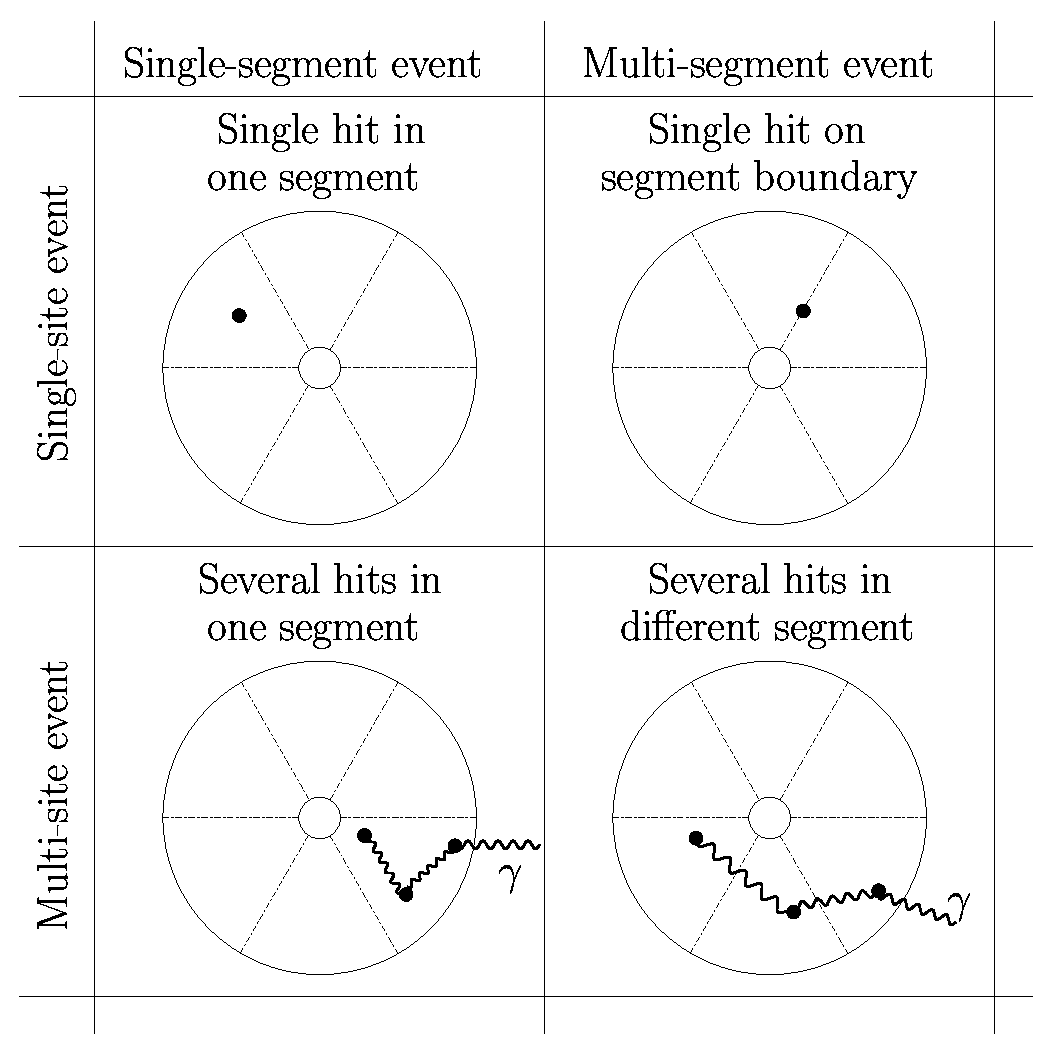
\includegraphics[width=0.5\textwidth]{events}
\caption{Possible event configurations. The cross section of a
Siegfried-like detector is depicted. The black dots are hits (energy
deposits). The wavy lines indicate $\gamma$-rays.}
\label{fig:ph:eve}
\end{figure}

\section{Background rejection using segmentation}
\label{sec:ph:seg}
Different data samples were taken using the segmented germanium
detector Siegfried I (see Sec.~\ref{sec:gerda:stat3}) and its test
stand (see Sec.~\ref{sec:tt:comc}) with $^{228}$Th and $^{60}$Co
$\gamma$ sources placed 10~cm above the vacuum cryostat (see
Fig.~\ref{fig:tt:comcryo}). Figure~\ref{fig:ph:seg} taken from
Ref.~\cite{Pid07} shows the core energy spectrum of the $^{228}$Th
data sample for all events (black) and single-segment events
(grey). The double escape peak\footnote{A double-escape-peak event is
created as follows: a photon produces a pair of electron and positron
inside the detector, the positron losses all its energy and
annihilates with another electron resulting in two 511~keV photons,
and both of the photons escape from the detector. Since the energy is
deposited only by an electron and a positron within a small region,
the double-escape-peak event is a single-site event.} (DEP in short)
from $^{208}$Tl ($1\,593$~keV) is hardly suppressed since the DEP
events are mostly single-segment events; while the $^{212}$Bi line
($1\,620$~keV) is suppressed by a factor of $2.85 \pm 0.01$ since most
of the events inside the peak are photon induced multi-segment events.

\begin{figure}[htbp]
\centering
\subfloat[]{\label{fig:ph:sega}
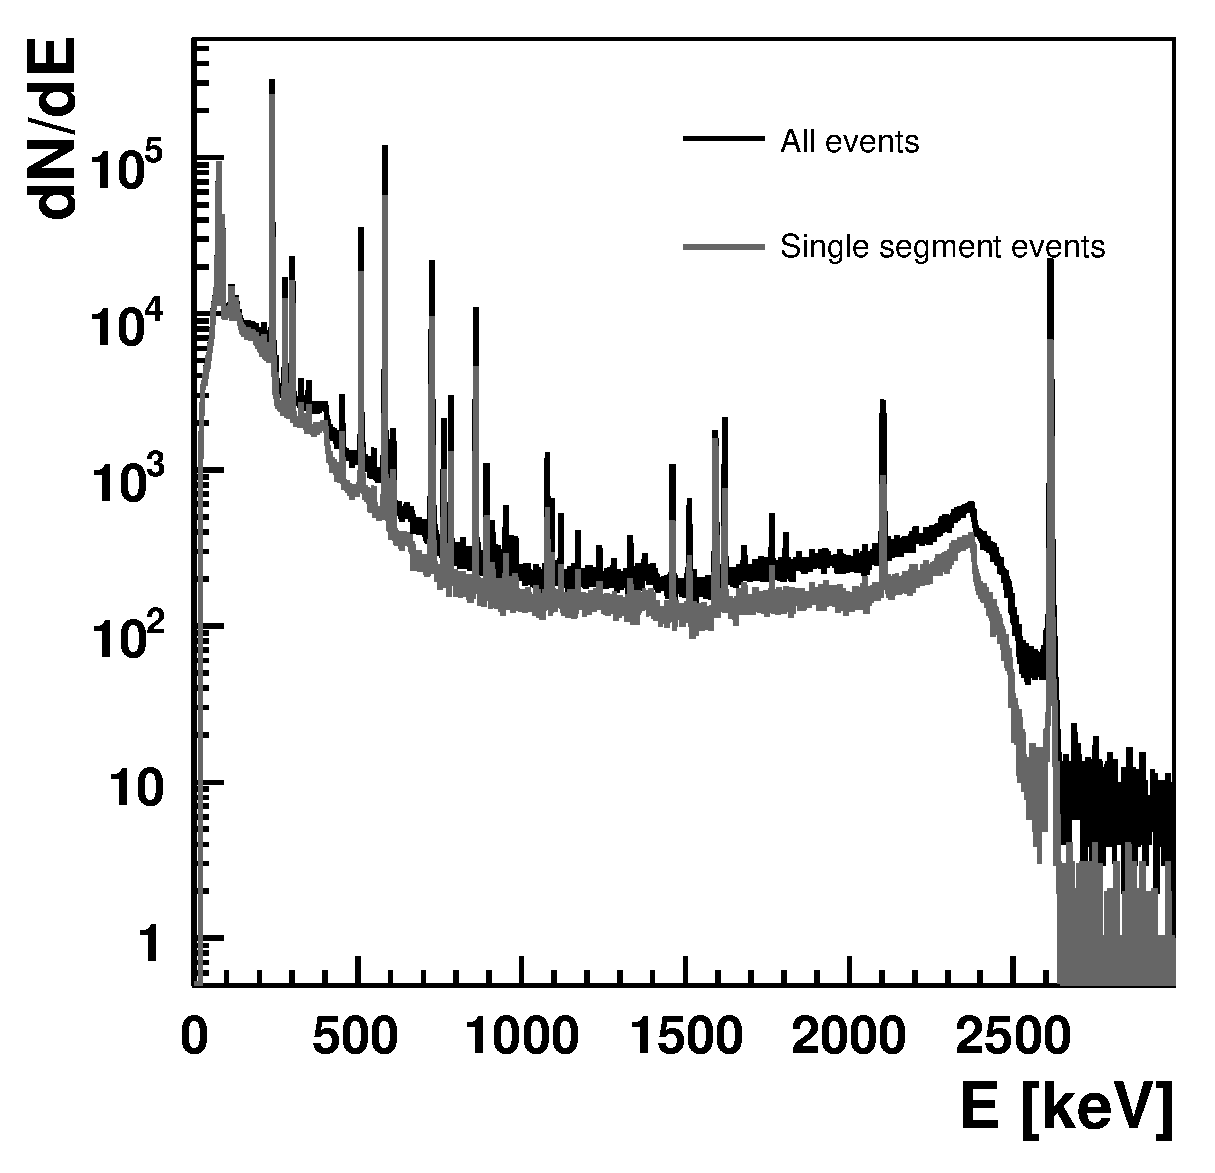
\includegraphics[width=0.4\textwidth]{energy_th228_suppression_all}}%
\subfloat[]{\label{fig:ph:segb}
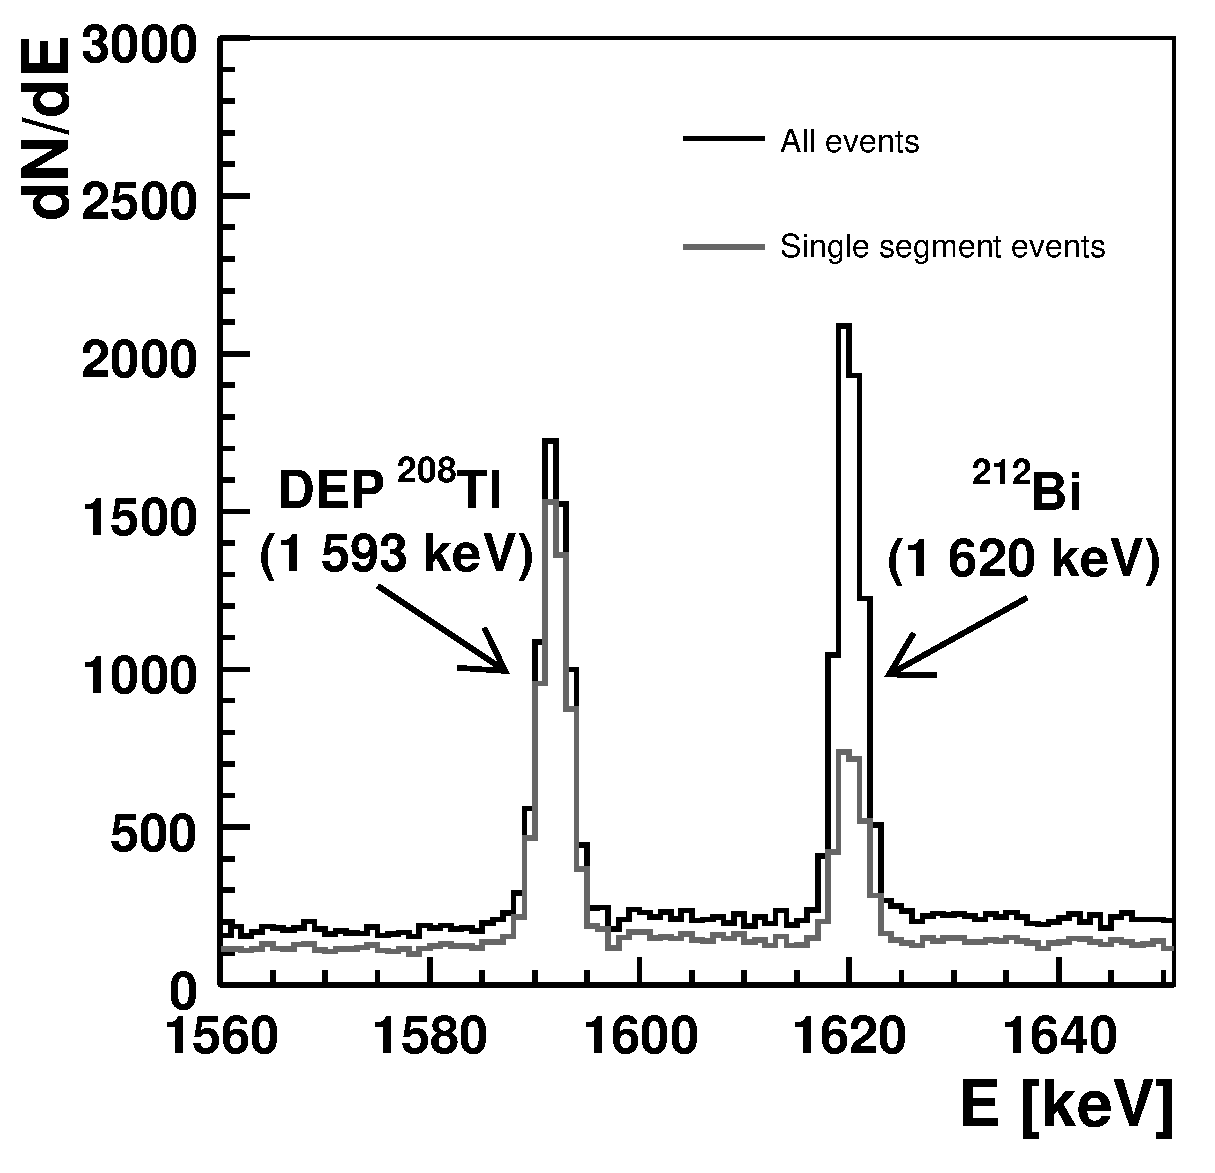
\includegraphics[width=0.4\textwidth]{energy_th228_suppression_ROI}}%
\caption{Core energy spectrum of the $^{228}$Th source data sample for
all events (black) and single-segment events (grey): (a)core spectrum
up to 3~MeV and (b) core spectrum around 1.6~MeV.}
\label{fig:ph:seg}
\end{figure}

\section{Monte Carlo simulation}
\label{sec:ph:sim}
Monte Carlo (MC) simulations of prototype detectors and their
cryostats were performed using MaGe \cite{Mag06, Mag08}, a C++ package
co-developed by the Majorana and GERDA collaborations using the Geant4
toolkits \cite{Gea03, Gea06}. Figure~\ref{fig:ph:sim} shows the
geometrical models of the detectors and cryostats implemented in
Geant4. Figure~\ref{fig:ph:s2} shows a close-up of Siegfried~II. It
was modeled in such a way that the details were implemented as close
as possible to reality while the speed of simulation did not decrease
too much.
 
\begin{figure}[tbhp]
\centering
\subfloat[]{\label{fig:ph:s1}
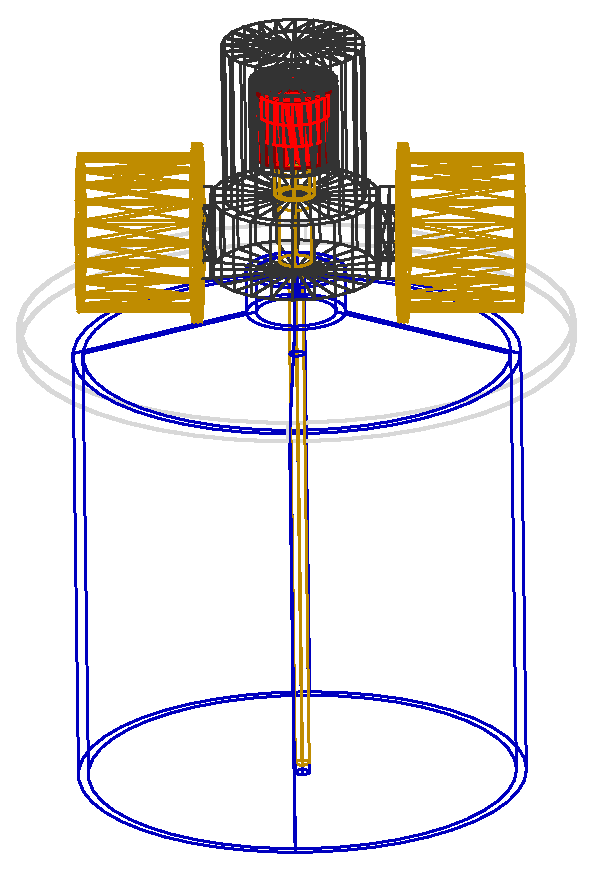
\includegraphics[height=0.25\textheight,clip]{SIwired}}
\subfloat[]{\label{fig:ph:g2}
  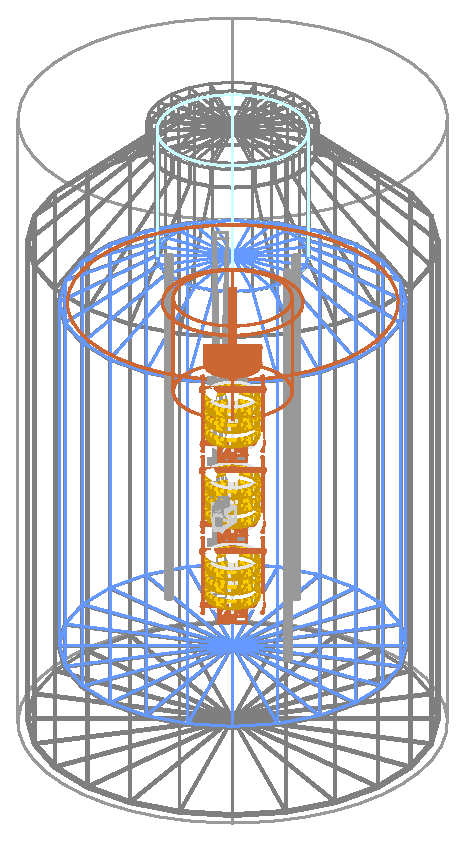
\includegraphics[height=0.25\textheight,clip]{GIIwired}}
\subfloat[]{\label{fig:ph:s2}
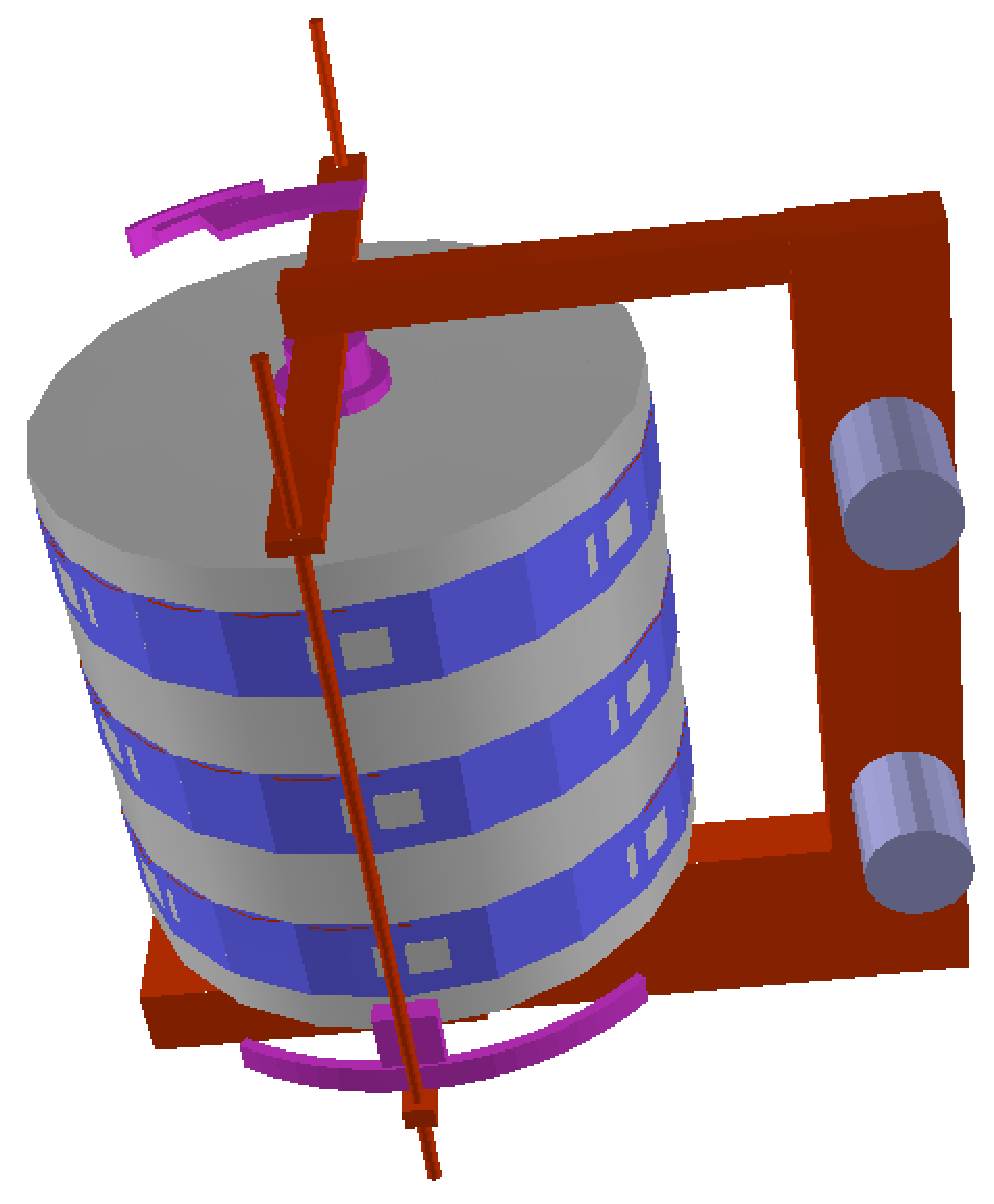
\includegraphics[height=0.2\textheight,clip]{SIIsolid}}
\caption{Geant4 models for detectors and their test stands: (a) wire
drawing of Siegfried~I and its cryostat, (b) wire drawing of GII, and
(c) a close-up of Siegfried~II with the copper frame as used in GII.}
\label{fig:ph:sim}
\end{figure}

The energy deposits of hits in each segment were recorded and the core
energy was calculated by adding all segment energies. The segment and
core energies were individually smeared according to the energy
resolutions of the detectors measured in the individual channels.

The spatial and time information of hits were also recorded and served
as parts of the input for the pulse shape simulation package. The
geometry of detectors and the voltage bias applied were other input
information for the pulse shape simulation. The details of the pulse
shape simulation are described in Chapter~\ref{cha:pss}.

\section{Verification of the Monte Carlo}
\label{sec:ph:var}

The simulation of photon interactions was done with Geant4.8.1 patch
2, and verified for (a) the energy spectrum, (b) the occupancy of each
segment, namely, the number of events recorded by each segment (see
Fig.~\ref{fig:ph:occ} for measurement setup), (c) the multiplicity,
namely, the number of segments having signals, and (d) the line
suppression factors (SF$_{\text{L}}$) defined as the ratio of the
total number of events to the number of single-segment events within
the energy window $[E_{\gamma} - 3\sigma, E_{\gamma} + 3\sigma]$,
where $E_{\gamma}$ is the central energy of the gamma line and
$\sigma$ is the energy resolution of the line.\footnote{The
suppression factors were calculated after the background was
subtracted.} The simulated distributions of (a), (b) and (c) were
added to the background distribution measured, and then compared to
the data as shown in Fig.~\ref{fig:ph:mc}a, b and c. The line
suppression factors were calculated for data and MC, respectively, and
then compared to each other as shown in Fig.~\ref{fig:ph:mcd}.

\begin{figure}[htpb]
\centering
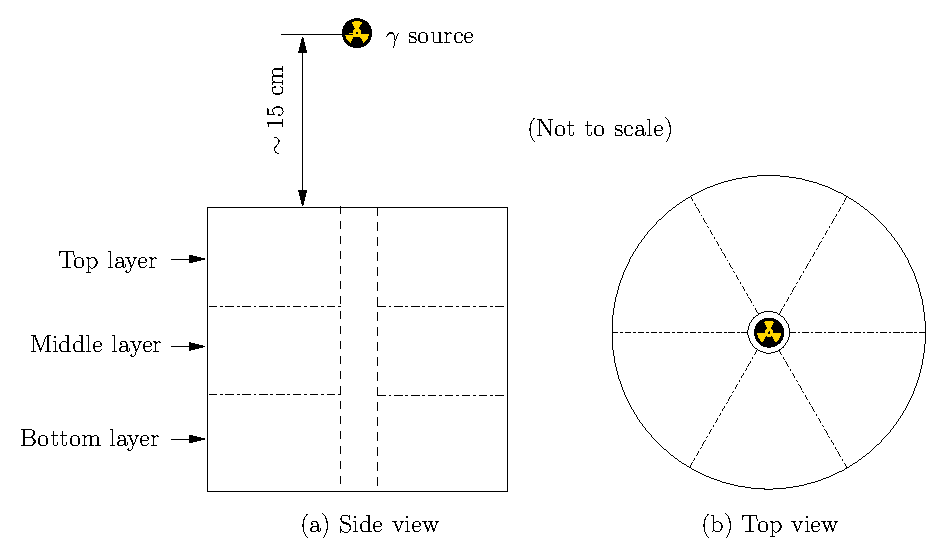
\includegraphics[width=0.65\textwidth]{occumea}
\caption{Schematic of experimental setup for occupancy measurement.}
\label{fig:ph:occ}
\end{figure}

\begin{figure}[htbp]
\centering
\subfloat[]{\label{fig:ph:mca}
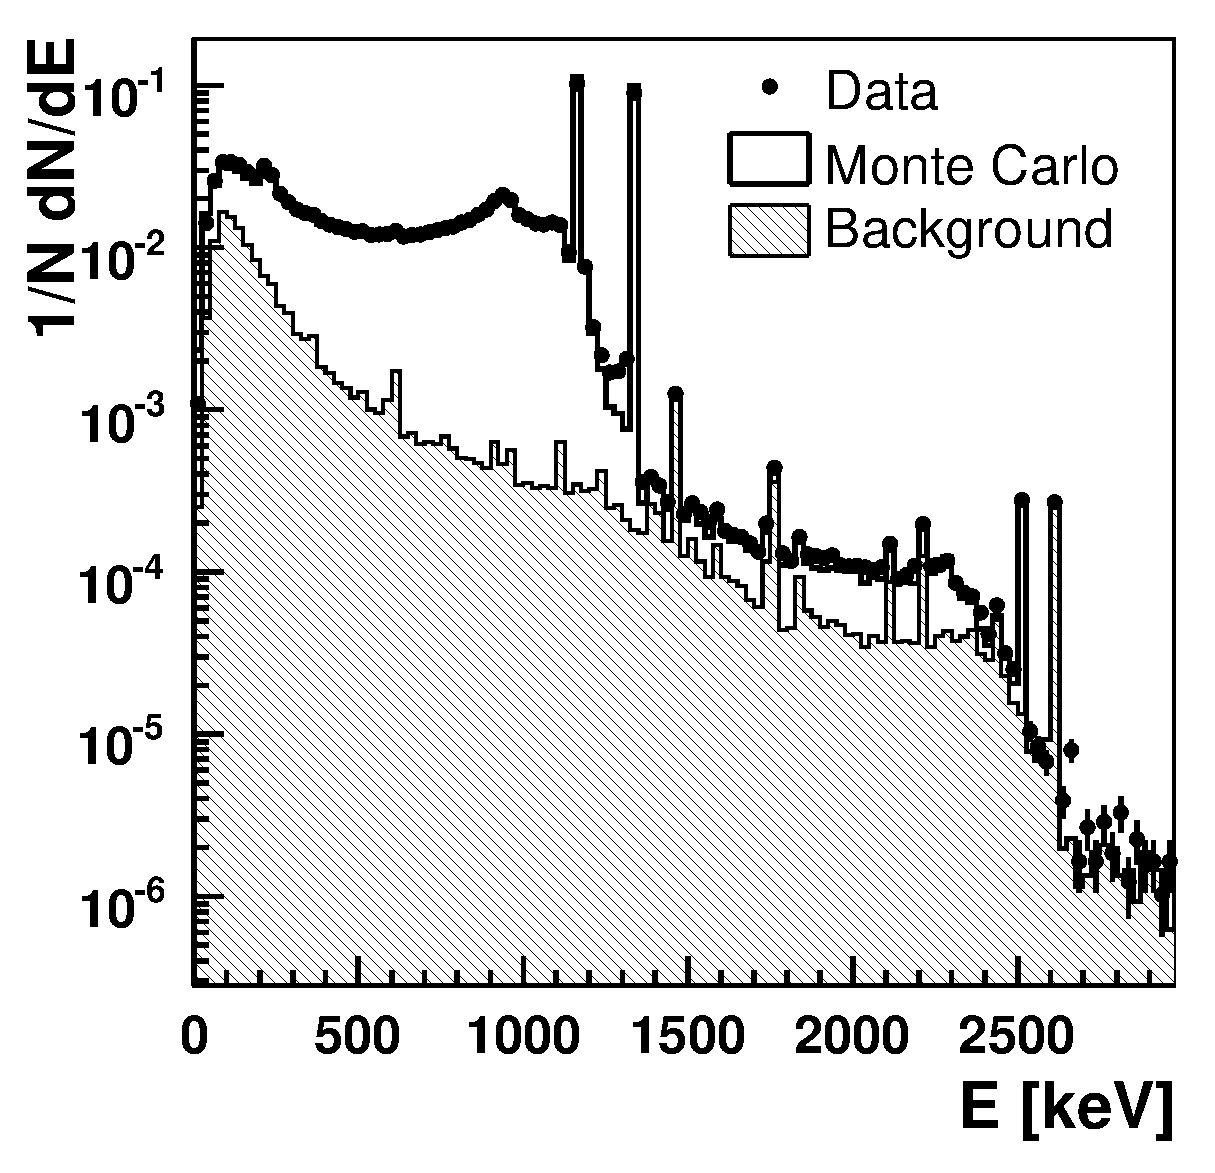
\includegraphics[width=0.45\textwidth]{datatomc_core_energy}}%
\subfloat[]{\label{fig:ph:mcb}
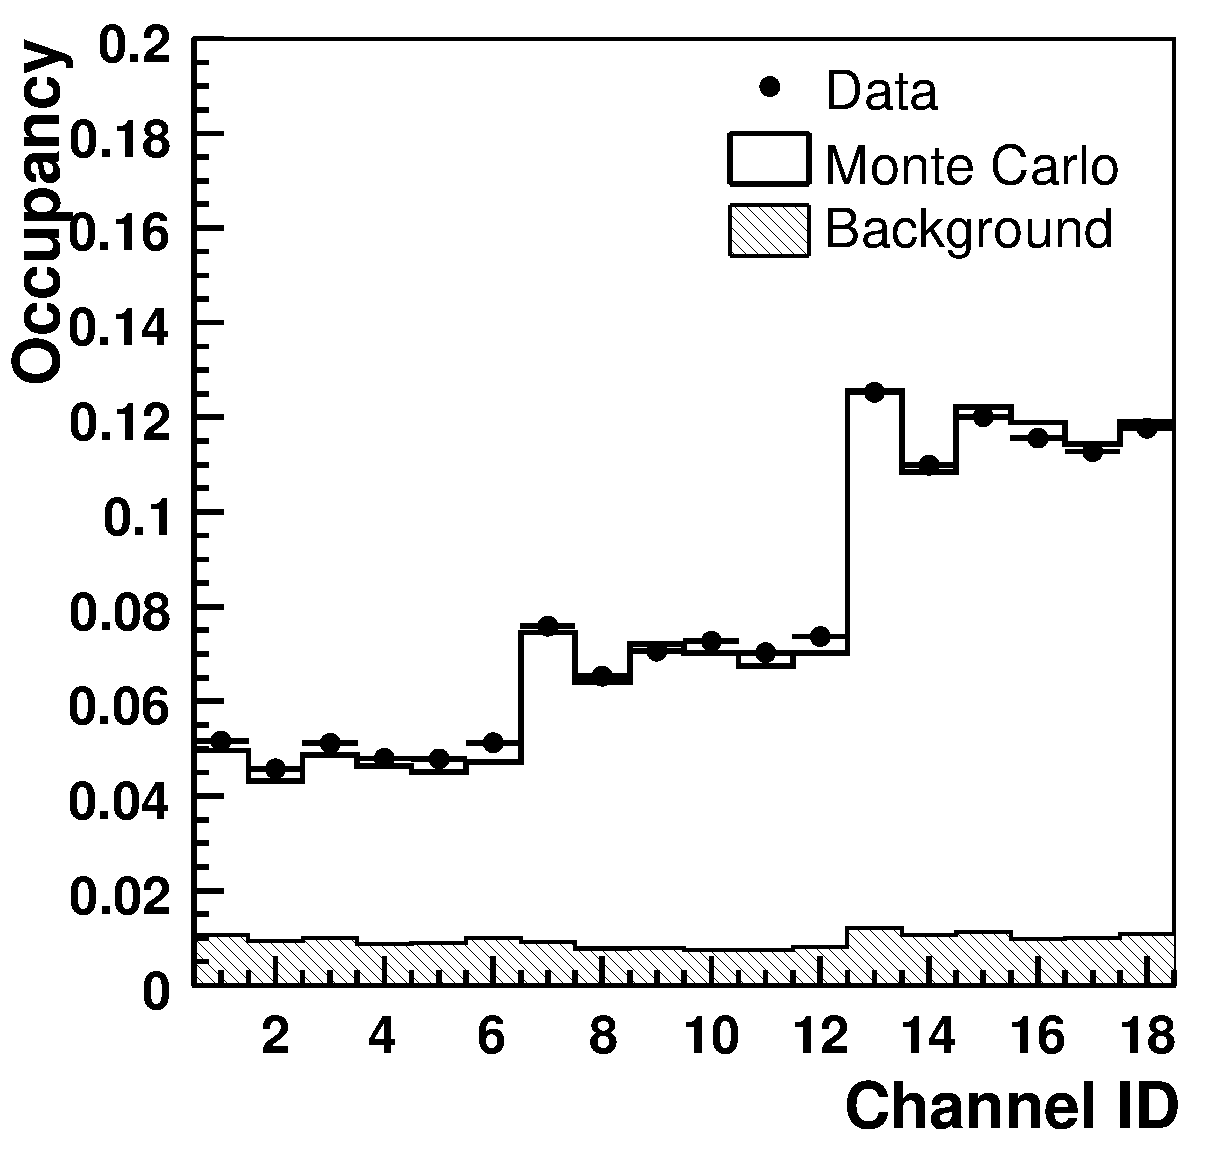
\includegraphics[width=0.45\textwidth]{datatomc_occupancy}}\\
\subfloat[]{\label{fig:ph:mcc}
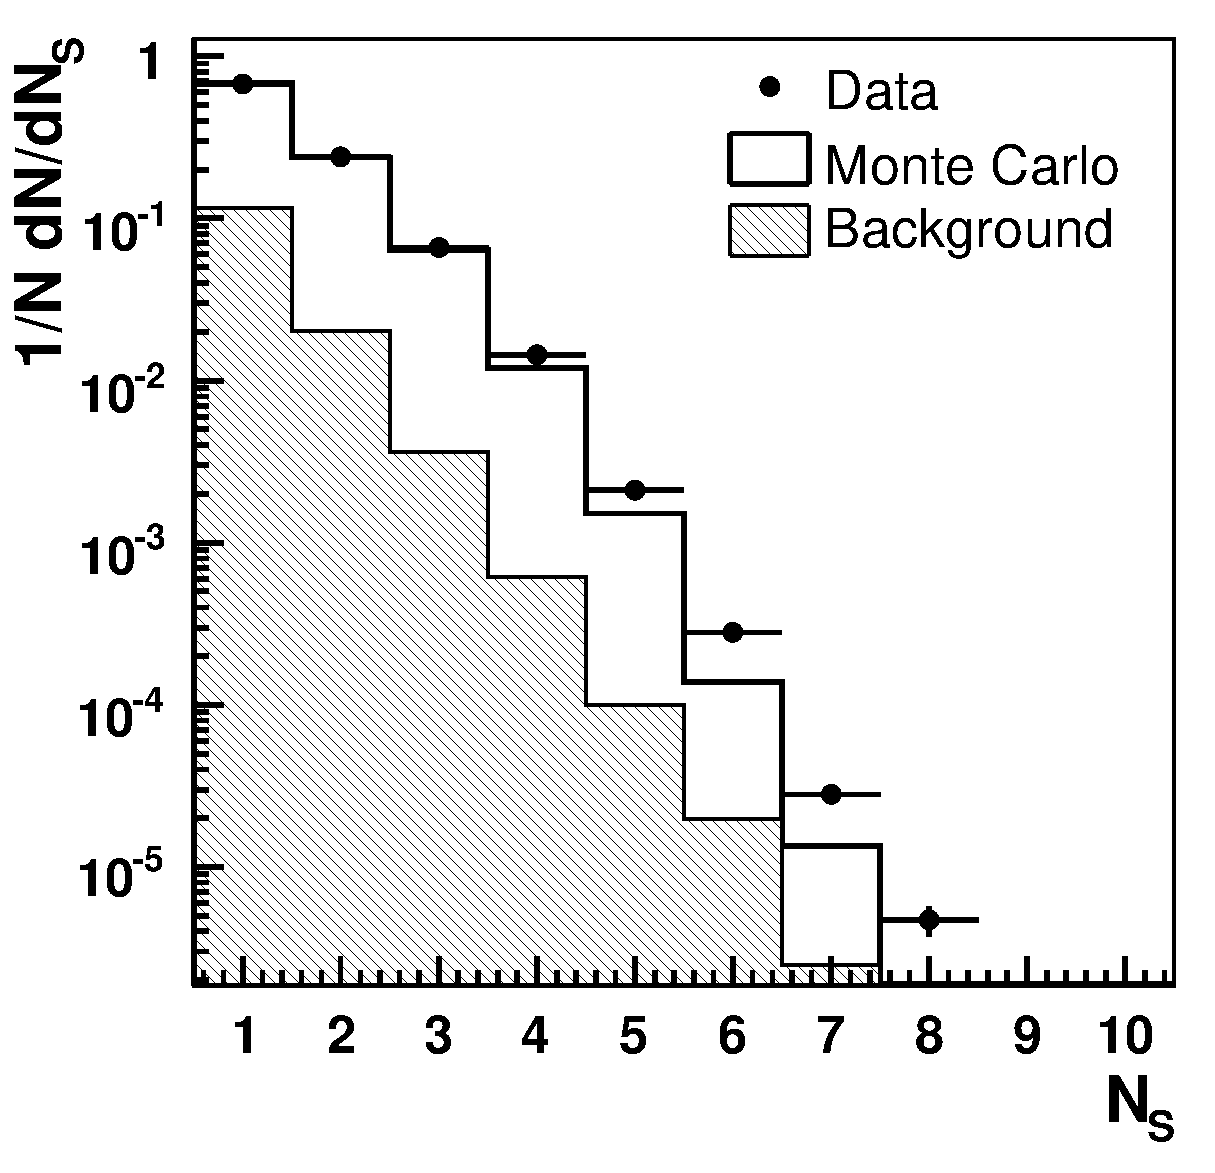
\includegraphics[width=0.45\textwidth]{datatomc_multiplicity}}%
\subfloat[]{\label{fig:ph:mcd}
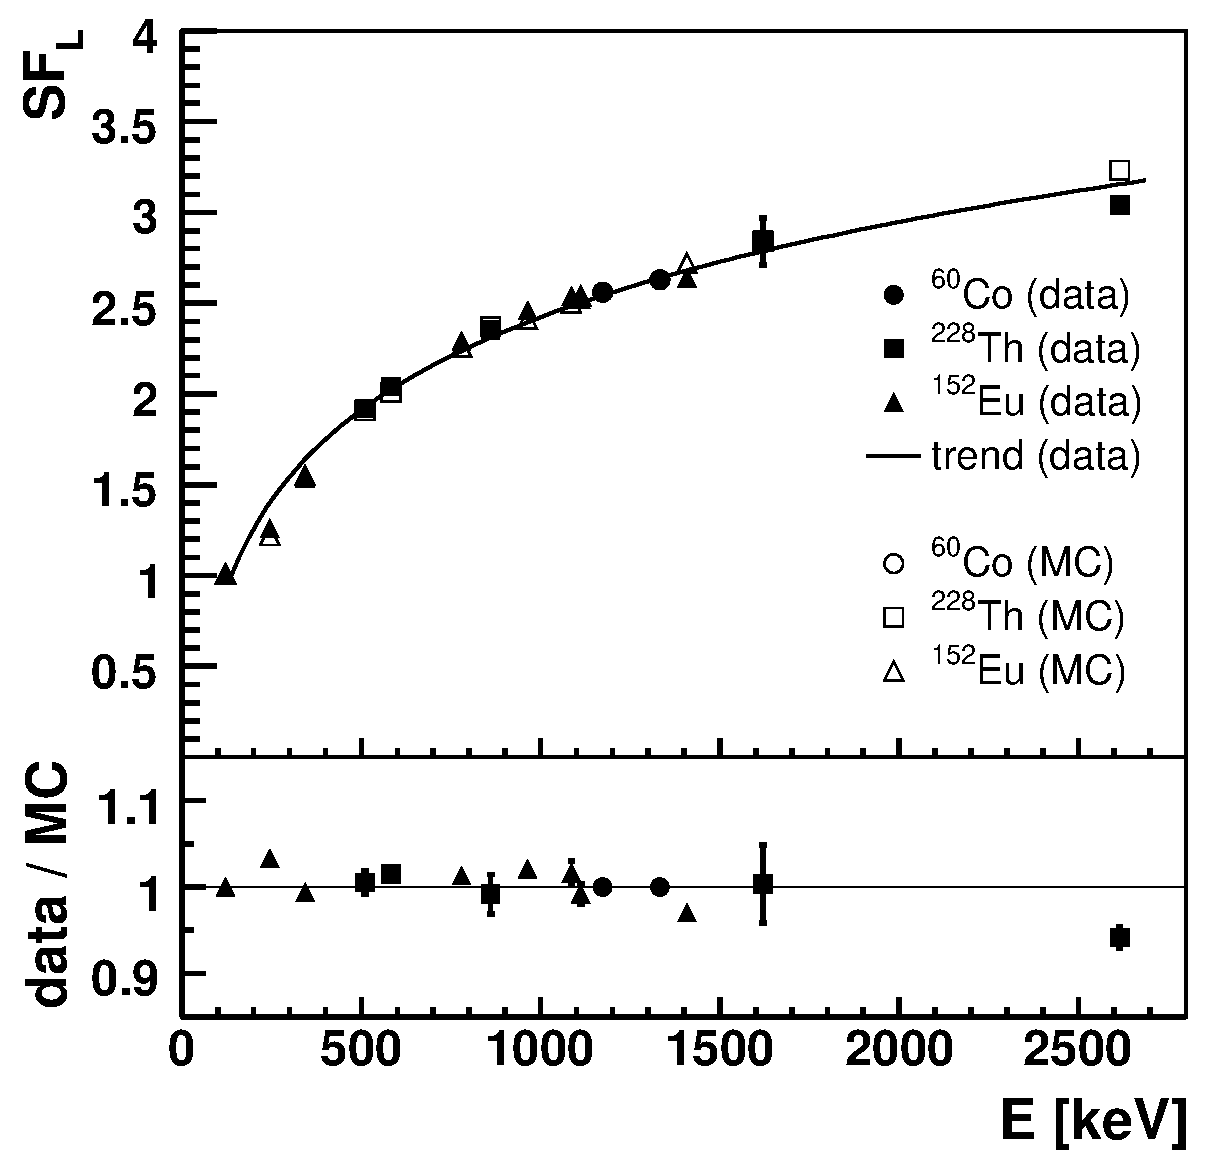
\includegraphics[width=0.45\textwidth]{suppression}}%
\caption{Comparison between data (dots with error bars) and MC (open
histogram) plus background (hatched histogram) for several quantities
under study: (a) core energy spectrum, (b) occupancy of all segments,
(c) segment multiplicity and (d) suppression factors. Plots are taken
from Ref.~\cite{Pid07}.}
\label{fig:ph:mc}
\end{figure}

The MC simulation agrees very well with the data in general. However,
there are some discrepencies observed in different aspects.

As shown in Fig.~\ref{fig:ph:mca}, the low energy side of the 1332~keV
peak in the data is significantly higher than in MC. This could be due
to the surface channel effect as described in Sec.~\ref{sec:np:exp}.

The occupancy distribution as shown in Fig.~\ref{fig:ph:mcb} was
measured with the experimental setup shown in
Fig.~\ref{fig:ph:occ}. The $\gamma$ source was placed above the center
of the detector. Naturally, the top layer of the detector (segment
No. 13 - 18\footnote{The segment naming scheme used here is different
from that shown in Fig.~\ref{fig:ger:segm} so that segments in the
same layer can be plotted aside each other.}) had the highest event
rates, the bottom layer (segment No. 1 - 6) had the lowest event
rates. The event rates of different segments in the same layer should
have been equal because the distance between the source and any of the
segments was the same (see Fig.~\ref{fig:ph:occ}b). However, this is
not the case as shown in Fig.~\ref{fig:ph:mcb}. This is because the
drift of charge carriers is affected by the structure of the germanium
crystal; the drift trajectories do not exactly follow the electric
field lines. This effect cannot be simulated using Geant4. An
effective model was used to tune the simulated distribution in order
to minimize the discrepancy between MC and data. The development of a
full simulation of the drift of the charge carriers in germanium
detectors is described in Chapters~\ref{cha:pss} and \ref{cha:psa}.

There is a deviation of 5\% between data and Monte Carlo plus
background data for multiplicities up to three. For higher
multiplicities the data exceeds the Monte Carlo with increasing
multiplicity. This may due to the fact that a hit close to the segment
boundary is always assigned to one segment in simulation while in
reality it may induce signals in several segment nearby.

%%% Local Variables:
%%% mode:latex
%%% TeX-master: "thesis"
%%% End:

\chapter{Neutron induced background}
\label{cha:neutron}
%$Id$

\section{Introduction}
\label{sec:neu:intro}
Neutrons produced near the germanium detectors by penetrating cosmic-ray muons can induce background events. In addition, neutrons from $(\alpha, n)$ reactions in the surrounding rock are also a potential source of background. The study of neutron interactions with germanium isotopes as well as the surrounding materials is thus of great interest.

Segmented germanium detectors will be used in GERDA Phase II. It has been shown that segment information is very useful to identify photon induced background~\cite{Pid07}. It is interesting to check if segment information can also help with the identification of neutron induced background.

In order to study the issues mentioned above, a GERDA Phase II 18-fold segmented prototype detector~\cite{Sie07} was exposed to an AmBe neutron source. Energy spectra were recorded for each segment and the core. The segment information was used to identify peaks induced by neutron interactions.

The Geant4~\cite{Gea03,Gea06} based simulation package, MaGe~\cite{Mag06, Mag08}, has been co-developed by the GERDA and MAJORANA~\cite{Gai03, Aal04} collaborations. The simulation of neutron interactions was verified by comparisons to data.

\section{Experimental setup and data sets}
\label{sec:neu:exp}
The detector used is the first segmented GERDA prototype detector. The
n-type true coaxial cylindrical crystal made of natural germanium has
a height of 70~mm and a diameter of 75~mm with a 10~mm hole in the
center. It is 18-fold segmented with a 6-fold segmentation in the
azimuthal angle $\phi$ and a 3-fold segmentation in the height $z$.
The resolution of the segments at 1.3~MeV is $\sim3$~keV. The total
energy resolution (core resolution) at 1.3~MeV is $4.07 \pm 0.03$~keV.
It was operated in a conventional test cryostat. Details of the
detector and its cryostat can be found in \cite{Sie07}.

A 1.1~GBq isotropic AmBe neutron source was used in the experiment.
The energy spectrum of the neutrons emitted from the
$^{9}$Be$(\alpha,n)^{12}$C$^{*}$ nuclear reaction extends to 12~MeV.
High resolution measurements of the neutron energy spectra of this
kind of neutron source are presented in~\cite{Mar95,Gei75}. The
dependence of the emittance of photons from the de-excitation of
$^{12}$C$^{*}$ on the neutron energy is described in~\cite{Gei75}.

The neutron source was located in a cylindrical paraffin
collimator. The schematic experimental setup (not to scale) is shown
in Fig.~\ref{fig:neu:exp}. The center of the collimator was vertically
aligned to the center of the detector and the distance between source
and detector center was about 1~m.

\begin{figure}[tbhp]
  \centering
  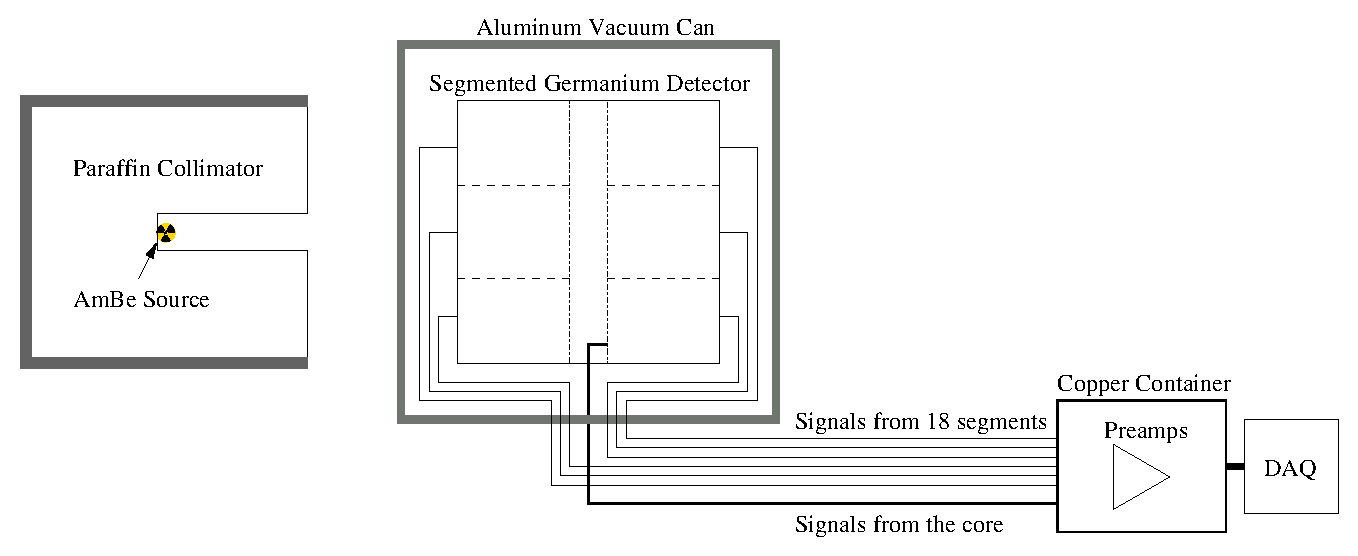
\includegraphics[width=0.8\textwidth]{neuExpSI}
  \caption{Schematic experimental setup (not to scale).}
  \label{fig:neu:exp}
\end{figure}

The core and segment electrodes were connected to charge sensitive pre-amplifiers. Their output was digitized using 14-bit ADCs in an XIA Pixie-4 data acquisition system~\cite{Daq06} with a sampling rate of 75~MHz, and recorded separately when the core was triggered. The system was configured such that if two pulses occured within 240~ns they were added up to a single signal; if the second pulse occured 240~ns to 8~$\mu$s after the first one, it was disregarded. Two different gain factors were chosen for four different measurements. The data sets are listed in Table~\ref{tab:neu:datset}. A low gain factor was chosen so that the energy range up to $\sim 11$~MeV could be covered. A high gain factor was chosen for measurements up to $\sim 3$~MeV.

Two measurements were performed with the AmBe source present. They are
referred to as HGdat (High Gain data) and LGdat (Low Gain data). In
order to determine the background from the laboratory environment two
more measurements without the source were performed. They are referred
to as HGbg (High Gain background) and LGbg (Low Gain background). The
data samples with different gains were combined for the study below
3~MeV.

\begin{table}[tbhp]
  \caption{Data sets recorded with and without source.} 
  \label{tab:neu:datset}\centering
  \begin{tabular}{lcccc}\hline
    & \multicolumn{2}{c}{With AmBe Source} &
\multicolumn{2}{c}{Without AmBe Source} \\
    \hline
    DAQ Gain & High  & Low   & High  & Low  \\
    $E_{max}$ [MeV] & $\sim$ 3.5  & $\sim$ 11 & $\sim$ 3.5 & $\sim$ 11
\\
    No. of Events & 7.1 M & 4.7 M & 1.5 M & 4.7 M \\
    Name & HGdat & LGdat & HGbg & LGbg \\\hline
  \end{tabular}
\end{table}

\section{Core spectra}
\label{sec:neu:spec}
The total energy deposited in the germanium crystal was read out from the core electrode of the detector. Figure~\ref{fig:neu:spec} shows the core energy spectra for the data and background in the range of [0.08, 3]~MeV. The thick line indicates the sum of HGdat and LGdat. The fine line represents the normalized sum of HGbg and LGbg. The trigger thresholds were set such that the spectra above 100~keV were not affected.

Eight photon peaks from the background were fitted with a Gaussian
function plus a first order polynomial to normalize the background to
the data.  They are associated with the decays of $^{214}$Pb
(352~keV), $^{214}$Bi (609~keV, 1120~keV, 1764~keV, 2448~keV),
$^{228}$Ac (911~keV), $^{40}$K (1461~keV), and $^{208}$Tl (2615~keV).
The numbers of events in the peaks determined by the fits were used to
calculate the data to background ratios. The average of these ratios,
$1.279 \pm 0.003$, was then used to scale the background spectrum.

\begin{figure}[tbhp]
  \centering
  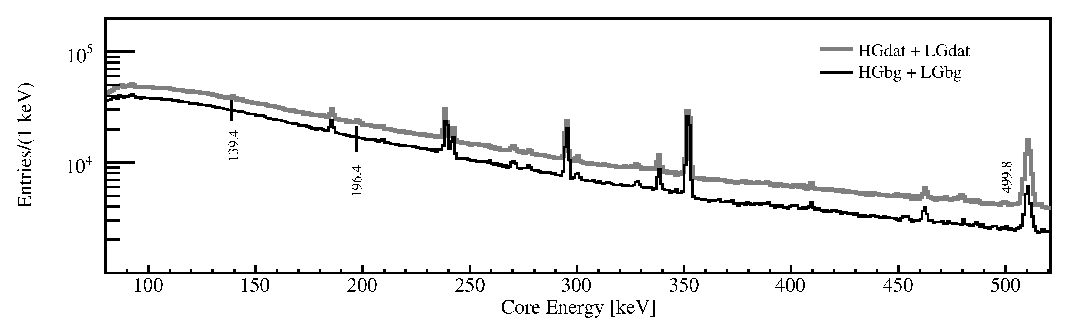
\includegraphics[width=0.8\textwidth,clip]{spectra_0_520keV}
  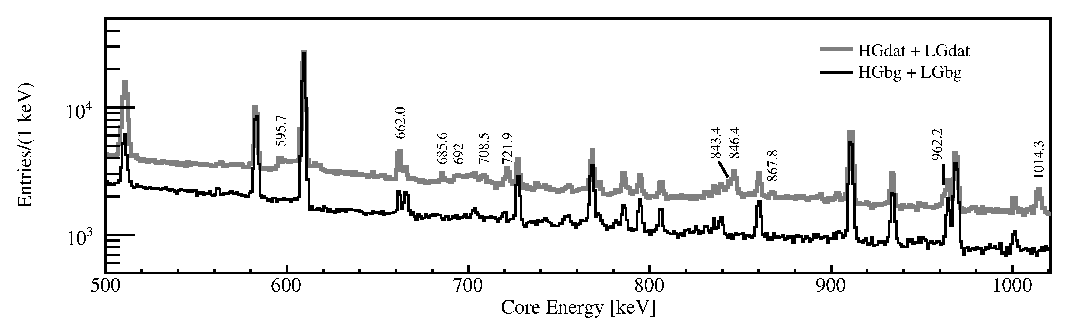
\includegraphics[width=0.8\textwidth,clip]{spectra_500_1020keV}
  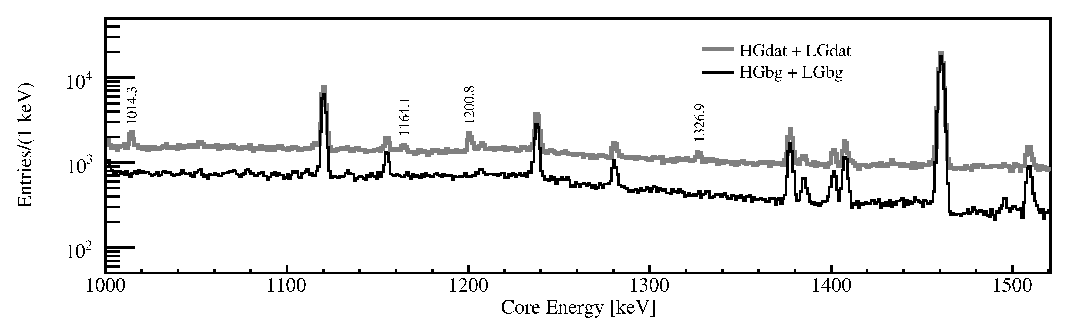
\includegraphics[width=0.8\textwidth,clip]{spectra_1000_1520keV}
  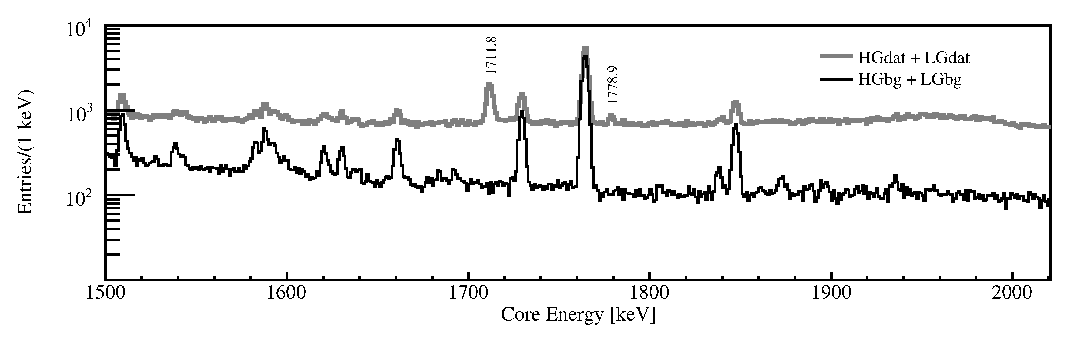
\includegraphics[width=0.8\textwidth,clip]{spectra_1500_2020keV}
  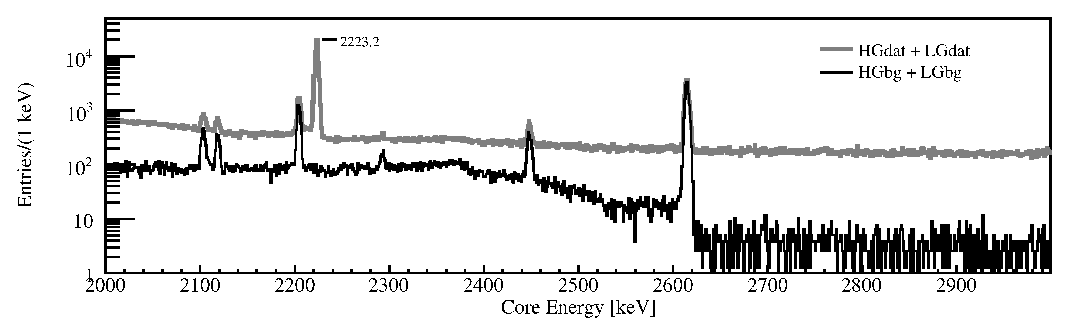
\includegraphics[width=0.8\textwidth,clip]{spectra_2_3MeV}
  \caption{Core energy spectra with and without source. The
    normalization procedure is described in the text. The energy range
    is [0.08, 3]~MeV. Peaks induced by the AmBe source are indicated
    with their energies.}
  \label{fig:neu:spec}
\end{figure}

Figure~\ref{fig:neu:specl} shows the spectra in the range of [3,
10.2]~MeV. In this energy range the background is small, as there are
hardly any natural radioactive elements producing photons with such
high energies.

\begin{figure}[tbhp]
  \centering
  \includegraphics[width=0.8\textwidth,clip]{spectra_3_11MeV}
  \caption{Core energy spectra with and without source. The
    normalization procedure is described in the text. The energy range
    is [3, 10.2]~MeV. Peaks induced by the AmBe source are indicated
    with their energies.}
  \label{fig:neu:specl}
\end{figure}

To illustrate the neutron interactions more clearly the normalized
background was subtracted from the data. This is shown in
Fig.~\ref{fig:neu:specd}. Some of the less prominent structures were
washed out since a larger bin width was chosen.

\begin{figure}[tbhp]
  \centering
  \includegraphics[width=0.8\textwidth,clip]{spectra_0_1d5MeV}
  \includegraphics[width=0.8\textwidth,clip]{spectra_1d5_3MeV}
  \includegraphics[width=0.8\textwidth,clip]{spectra_3_10d2MeV}
  \caption{Core energy spectra with background subtracted.}
  \label{fig:neu:specd}
\end{figure}

\section{Neutron interactions as seen by the core}
\label{sec:neu:type}
The main interaction mechanisms of neutrons with energies less than 12~MeV are thermal capture, inelastic and elastic scattering. Elastic scattering does not induce peaks that can be identified, because there is no photon emitted and the recoil energy distribution is too flat. Not only the production mechanism of the excited nucleus is important for the identification of a peak. The de-excitation mechanism has also to be taken into account. In most cases the nucleus de-excites instantaneously with the emission of one or more photons. However, it can also undergo internal conversion, in which case an electron from a lower shell is emitted instead of a photon. The excited nucleus can also be meta-stable and not de-excite instantaneously.

Table~\ref{tab:neu:type} lists the processes identified in the core energy spectrum. If inelastic scattering happens inside the germanium crystal, the nuclear recoil energy is recorded as well as the energies from some of the prompt photons. In case of instantaneous de-excitation they are summed up: $E_{inelastic} = E_{\gamma} + E_{recoil}$. This causes an asymmetric peak with a long recoil tail on the high energy side. Internal conversions only create identifiable peaks, if they occur inside the crystal, otherwise the emitted electrons do not reach the detector.

\begin{table}[tbhp]
  \caption{Type of neutron processes identified in the core energy
spectrum.}
  \label{tab:neu:type}\centering
  \begin{tabular*}{\textwidth}{@{\extracolsep{\fill}}cccc}
    \hline\noalign{\smallskip}
    Production & De-excitation & Symbolic Notation & Short Form \\
    \noalign{\smallskip}\hline\noalign{\smallskip}
    thermal & instantaneous & $n + ^A$Z$ \rightarrow ^{(A+1)}$Z$ +
\gamma$ & $^A$Z$(n,\gamma)$\\
    \noalign{\smallskip}\cline{2-4}\noalign{\smallskip}
    capture & meta-stable 
    & $n + ^A$Z$ \rightarrow ^{(A+1)m}$Z, $^{(A+1)m}$Z$ \rightarrow
^{(A+1)}$Z$+\gamma$ & $^A$Z$(n,\gamma^{m})$\\
    %& & $^{(A+1)m}$Z$ \rightarrow ^{(A+1)}$Z$+\gamma$ & \\
    \noalign{\smallskip}\hline\noalign{\smallskip}
    inelastic & instantaneous & 
    $n + ^A$Z$ \rightarrow ^A$Z$ + n^\prime + \gamma$ &
$^A$Z$(n,n^\prime\gamma)$\\
    \noalign{\smallskip}\cline{2-4}\noalign{\smallskip}
    scattering & internal conversion & 
    $n + ^A$Ge$ \rightarrow ^A$Ge$^{+} + n^\prime + e^-$ &
$^A$Ge$(n,n^\prime e)$\\
    \noalign{\smallskip}\hline
  \end{tabular*}
\end{table}

Table~\ref{tab:neu:peak}, \ref{tab:neu:peak2} list all the peaks observed in the core energy spectrum due to neutron interactions within the germanium crystal as well as within the surrounding materials: H, C, Cl in the paraffin collimator, Al, Ce in the aluminum vacuum can, and Fe, Cu in the supporter and container of the detector and electronics.

Pure photon peaks were fitted with a Gaussian function plus a first order polynomial to get the mean energies, FWHMs and the numbers of events in the peaks. The 596~keV peak from $^{74}$Ge$(n, n^\prime \gamma)$ does not have a Gaussian distribution. The treatment of this peak will be described in section~\ref{sec:neu:seg}. The 662~keV peak associated with $^{140}$Ce has a significant background contribution from $^{137}$Cs. This was subtracted. The 692~keV peak from $^{72}$Ge$(n,n^\prime e)$ is hard to fit because it is asymmetric and broad. It is also contaminated by other peaks nearby. The number of events in this peak was estimated by integration.

The 4.4 MeV peak is due to photons from the de-excitation of $^{12}$C$^{*}$ created in the AmBe source by the interaction, $^{9}$Be$(\alpha,n)^{12}$C$^{*}$. It is Doppler broadened because of the movement of the $^{12}$C$^{*}$ nuclei. The width of this peak listed in Table~\ref{tab:neu:peak2} was determined by the fit. Because of low statistics the widths of most of the peaks above 6 MeV had to be fixed in the fitting procedure according to the detector resolution around these energies. The peaks that are not identified are marked with a question mark.

\begin{table}[tbhp]
  \caption{Peaks observed in the core energy spectrum (see
Fig.~\ref{fig:neu:spec})
    due to neutron interactions.} 
  \label{tab:neu:peak}\centering
  \begin{minipage}{\linewidth}
    \begin{tabular}{llll} \hline
      Fitted Energy~[keV]& Fitted FWHM~[keV]& Interaction Type& Number of Events\\\hline
      139.4 & $1.6 \pm 0.2$ & $^{74}$Ge$(n,\gamma^m)$ & $3377 \pm 520$
\\
      197.9 & $1.9 \pm 0.2$ & $^{70}$Ge$(n,\gamma^m)$ & $3306 \pm 503$
\\
      499.8 & $1.9 \pm 0.7$ & $^{70}$Ge$(n,\gamma)$   & $503  \pm 186$
\\
      595.7\footnote{The fitting of the 596~keV peak is described in a
        later section.}
      & - & $^{74}$Ge$(n,n^\prime\gamma)$ & $(18.4 \pm 2.5)\times10^3$
\\
      662.0\footnote{The background contribution to the 662~keV peak
        was subtracted.}
      & $1.9 \pm 0.1$ & $^{140}$Ce$(n,\gamma)$ & $2802 \pm 188$ \\
      685.6 & $1.4 \pm 0.2$ & ?\footnote{The unidentified peaks are
        marked with a question mark.} & $628  \pm 111$ \\
      692\footnote{The number of events in the 692~keV peak was
        determined by integration.}  & - & $^{72}$Ge$(n,n^\prime e)$ &
      $\sim 7000$
      \\
      708.5  & $2.4 \pm 0.5$ & $^{35}$Cl$(n,\gamma)$,       & $782 
\pm 197$ \\
      &  & $^{36}$Cl$\rightarrow^{36}$Ar & \\
      721.9  & $1.9 \pm 0.2$ & ?$^c$ & $3502 \pm 148$ \\
      843.4  & $2.4 \pm 0.5$ & $^{27}$Al$(n,n^\prime\gamma)$ & $1558
\pm 202$ \\
      846.6  & $2.4 \pm 0.2$ & $^{56}$Fe$(n,n^\prime\gamma)$ & $2802
\pm 196$ \\
      867.8  & $1.9 \pm 0.5$ & $^{73}$Ge$(n,\gamma)$        & $425 
\pm 129$ \\
      962.2  & $2.4 \pm 0.2$ & $^{63}$Cu$(n,n^\prime\gamma)$ & $1041
\pm 129$ \\
      1014.3 & $2.4 \pm 0.2$ & $^{27}$Al$(n,n^\prime\gamma)$ & $1958
\pm 123$ \\
      1164.1 & $2.6 \pm 0.5$ & $^{35}$Cl$(n,\gamma)$        & $646 
\pm 140$ \\
      1200.8 & $2.8 \pm 0.2$ & DEP\footnote{SEP, DEP stand for Single
        Escape Peak and Double Escape Peak, respectively.} of 2223
      & $2318 \pm 122$ \\
      1326.9 & $2.4 \pm 0.2$ & $^{63}$Cu$(n,n^\prime\gamma)$   & $711 
\pm 91$  \\
      1711.8 & $3.8 \pm 0.1$ & SEP$^e$ of 2223 & $5555 \pm 133$ \\
      1778.9 & $2.6 \pm 0.2$ & $^{27}$Al$(n,\gamma)$, & $469  \pm 73$
\\
      &  & $^{28}$Al$\rightarrow^{28}$Si &  \\
      2223.2 & $3.8 \pm 0.1$ & $^{1}$H$(n,\gamma)$ & $79349 \pm 300$\\
    \end{tabular}
  \end{minipage}
\end{table}

\begin{table}[tbhp]
  \caption{Peaks observed in the core energy spectrum (see
Fig.~\ref{fig:neu:specl})
    due to neutron interactions.} 
  \label{tab:neu:peak2}\centering
  \begin{minipage}{\linewidth}\centering
    \begin{tabular}{llll} \hline\noalign{\smallskip}
      Fitted Energy~[keV]& Fitted FWHM~[keV]& Interaction Type& Number of Events\\\hline
 3427 & $85 \pm 7$
      & DEP\footnote{SEP, DEP stand for Single Escape Peak and Double
        Escape Peak, respectively.} of 4441 & $2354 \pm 263$ \\
      3931 & $87 \pm 5$  & SEP$^a$ of 4441 & $5873 \pm 368$ \\
      4441 & $92 \pm 2$  & $^{9}$Be$(\alpha,n)^{12}$C$^{*}$ & $14672
\pm 297$ \\
      4946 & $4.9\pm1.4$ & $^{12}$C$(n,\gamma)$            & $68 \pm
15$     \\
      6113 & 7\footnote{The widths were fixed during the fit.}
      & $^{35}$Cl$(n,\gamma)$ & $75 \pm 12$ \\
      6904 & 7$^b$      & SEP$^a$ of 7416            & $60 \pm 10$ \\
      7126 & 7$^b$ & ?\footnote{The unidentified peaks are marked with
        a question mark.} & $38 \pm  9$ \\
      7416 & 7$^b$       & $^{35}$Cl$(n,\gamma)$ & $70 \pm 10$ \\
      7633 & 7$^b$       & $^{56}$Fe$(n,\gamma)$ & $18 \pm 10$ \\
      7793 & $7.1\pm2.1$ & $^{35}$Cl$(n,\gamma)$ & $21 \pm  8$ \\
      7918 & $6.8\pm1.4$ & $^{63}$Cu$(n,\gamma)$ & $29 \pm  8$ \\
  \end{tabular}
  \end{minipage}
\end{table}

\section{Neutron interactions as seen by the segments}
\label{sec:neu:seg}
The energies deposited in each of the segments are read out
separately. This provides more information about the interactions
inside the germanium crystal than can be extracted from the core
signal alone.

For example, a photon with an energy of the order of one MeV has a
mean free path of several centimeters in the germanium crystal. It
most probably deposits energy in several different segments because of
multiple Compton scattering. The result is a \emph{multi-segment
  event}, in short MSE. In contrast, if there is only one segment with
an energy deposition, it is called a \emph{single-segment event}, in
short SSE. The power of discrimination of MSE and SSE induced by
photon using segmented germanium detectors has been shown in
\cite{Pid07}.

\subsection{Neutron inelastic scattering}
Compared to photon induced events, a special characteristic of neutron inelastic scattering in a germanium crystal is that not only the photon energy, but also the recoil energy, is recorded. The inelastic scattering peak in the core energy spectrum has a high energy recoil tail and, hence, is much less significant than a pure photon peak with the same number of events, as seen in Fig.~\ref{fig:neu:spec}. However, it is possible to partially separate out the recoil energy distribution using information from the individual segments. The disentangled photon peak is much more significant than the original peak. This is due to the way a segmented detector can provide information about event topologies.

Figure~\ref{fig:neu:inel} shows the three types of events contributing to the inelastic scattering peak in the core spectrum. In all cases the scattered neutron escapes:
\begin{enumerate}
\item The nuclear recoil energy and the prompt photon energy are
  deposited in the same segment;
\item The nuclear recoil energy is deposited within one segment, the
  prompt photon deposits its energy in several other segments;
\item The nuclear recoil energy is deposited within one segment while
  the prompt photon deposits its total energy within another segment.
\end{enumerate}

\begin{figure}[tbhp]
  \centering
  \includegraphics[width=0.8\textwidth]{ine_1}
  \caption{Three topologies of neutron inelastic scattering inside a
    germanium crystal.}
  \label{fig:neu:inel}
\end{figure}

In the first case, only one segment has a signal. The energies
recorded by the core and the segment are the same, i.e. $E_{core} =
E_{seg} = E_{\gamma} + E_{recoil}$. Segmentation cannot help to
disentangle the two energies. In the second case, the recoil energy
can be observed in one segment. As the photon energy is shared between
several segments, there is no peaked distribution in any single
segment. This would partially be recovered by segment energy
summation. In the third case, the recoil energy is observed in one
segment, while the photon is observed in another segment. To
disentangle the photon peak from the recoil energy distribution,
energy spectra of all the segments are summed to get a spectrum of the
energy deposited in \emph{any segment}. In this spectrum, the type~1
events produce the same distribution as in the core spectrum and type
2 events form a flat distribution. The type~3 events, however, create
a sharp photon peak at the original energy and an enhancement in the
low energy region, the recoil energy distribution.

Figure \ref{fig:neu:cas} shows the \emph{any segment} spectrum (fine line) together with the core spectrum (thick line) in the relevant energy ranges. Three peaks at 596~keV, 834~keV and 1039~keV, associated with inelastic scattering, $^{74}$Ge$(n, n^\prime\gamma)$, $^{72}$Ge$(n, n^\prime\gamma)$ and $^{70}$Ge$(n, n^\prime\gamma)$, respectively, are clearly visible in the \emph{any segment} spectrum. The latter two are washed out in the core spectrum.

\begin{figure}[tbhp]
  \centering
  \includegraphics[width=0.8\textwidth,clip]{spe_casp}
  \includegraphics[width=0.8\textwidth,clip]{spe_cas2p}
  \caption{The \emph{any segment} spectrum (fine line) and the core
    spectrum (thick line) in the relevant energy ranges. The inset
    shows a close-up of the 596~keV peak in the core spectrum. The
    fitting of recoil energy distribution is described in the text.}
  \label{fig:neu:cas}
\end{figure}


It is possible to extract the number of each type of events in the 596~keV peak. The core spectrum was used to determine the total number of events, $N_{total}$. An exponential function was fitted to the shoulder of the peak associated with the nuclear recoil energy distribution. A Gaussian function was fitted to the 609~keV background photon peak on the shoulder simultaneously. The background below the recoil structure was obtained from interpolating the spectrum below and above the shoulder. The total number of events equals to the difference between the fitted exponential and the background. The error was estimated by assuming different levels and shapes of the background. The fit is shown in the inset of Fig.~\ref{fig:neu:cas}. The dashed line represents the background, the solid line shows the exponential plus the Gaussian function from the background peak.

The number of type~3 events, $N_{type3}$, was obtained by fitting a
Gaussian function plus a first order polynomial to the 596~keV peak in
the \emph{any segment} spectrum. The small shoulder caused by the
contamination with type~1 events does not change the results of the
fit significantly.

In principle the number of type~1 events can be determined by fitting
the 596 keV peak in \emph{single segment} spectrum, which is obtained
by requiring only one segment having signal. However, a trigger
threshold bigger than 5~keV must be set for each segment in order to
avoid electric noise. Because the recoil energy is very likely to be
smaller than 5~keV a lot of type~3 events with recoil energy smaller
than 5~keV behave in reality as type~1 events. So the 596 keV peak in
\emph{single segment} spectrum contains all the type~1 events and a
large part of type~3 events.

Another way to determine the number of type~1 events requires the
study of the peaks purely induced by photons. This provides the
probability that a de-excitation photon deposits its energy in exactly
one or in multiple segments. The relative strength of the peaks in the
core and any segment spectrum, that is, $\mathcal{R}(E_{\gamma}) =
N_{core}(E_{\gamma}) / N^{any}_{seg}(E_{\gamma}) = (N_{SSE} + N_{MSE})
/ N_{SSE}$, directly translates to the relative rate of the total
number of inelastic scattering events to the sum of type~1 and type~3
events, that is, $\mathcal{R}(E_{\gamma}^{inelastic}) = N_{total} /
(N_{type1} + N_{type3})$.

A Gaussian function plus a first order polynomial were fitted to
eleven of the most prominent background photon induced peaks in the
core and \emph{any segment} spectra, respectively. The numbers of
events in the peaks from the fits were used to calculate the ratio,
$\mathcal{R}(E_{\gamma})$. The points with error bars in
Fig.~\ref{fig:neu:sf} represent the ratios calculated at different
energies. A second order polynomial was fitted to get an estimate of
the ratio at any energy, $\mathcal{R}(E)$. The number of type~1 events
can be calculated as $N_{type1} = N_{total} /
\mathcal{R}(E_{\gamma}^{inelastic}) - N_{type3}$.

\begin{figure}[tbhp]
  \centering
  \includegraphics[width=0.5\textwidth,clip]{sf}
  \caption{The ``core to any segment ratio'' as a function of the
    energy.}
  \label{fig:neu:sf}
\end{figure}

The number of type~2 events can then be calculated as $N_{type2} = N_{total} - N_{type1} - N_{type3}$. The results concerning event topologies in the 596~keV peak are listed in the second row of Table~\ref{tab:neu:ncore}. The percentage of single-segment events, that is, $N_{type1}$, out of the total number of events is $\mathcal{P} = N_{type1} / N_{total} \approx 5\%$.
\begin{table}[tbhp]
  \caption{Numbers of events in the 596~keV, 834~keV and 1039~keV
    peaks.    The two numbers in the square brakets indicate the     ranges of    numbers     of events with different topologies in     the     834~keV and 1039~keV    peaks.}
  \label{tab:neu:ncore}\centering
  \begin{minipage}{\textwidth}\centering
    \begin{tabular}{lcccc} \hline\noalign{\smallskip}
      Energy [keV]& $N_{type 1}$ & $N_{type 2}$  & $N_{type 3}$    &
$N_{total}$   \\
      \noalign{\smallskip}\hline\noalign{\smallskip} 595.8 &
      $1000 \pm 1000$ \footnote{The huge error is due to the
        propagation of errors of $N_{type1}$, $N_{total}$ and
        $\mathcal{R}$ according to the relation $N_{type1} = N_{total}
        / \mathcal{R} - N_{type3}$.}
      & $(10 \pm 3)\times10^3$ & $7285 \pm 218$ & $(18.4 \pm
2.5)\times10^3$ \\
      834.0  & [0, 380]    & [4100, 4700] & $2592 \pm 186$ & [6700,
7700] \\
      1039.2 & [0, 240]    & [2700, 3100] & $1429 \pm 182$ & [4100,
4800] \\
    \end{tabular}
  \end{minipage}
\end{table}

The numbers of type~3 events in the 834~keV and 1039~keV peaks were
obtained by fitting the \emph{any segment} spectrum. Since there is no
peak at these two energies in the core spectrum, it is impossible to
get $N_{total}$ from a fit. However, since the percentage $\mathcal{P}
= N_{type1} / N_{total}$ decreases with energy, $\mathcal{P}$ at
834~keV and 1039~keV should be less than $\mathcal{P}$(596~keV).
Taking into account the relation, $N_{type1} = N_{total}/\mathcal{R} -
N_{type3}$, the ranges of numbers of events in different topologies in
the 834~keV and 1039~keV peaks were calculated. They are listed in
Table~\ref{tab:neu:ncore} as well.

The following steps were used to disentangle the recoil energy
$E_{recoil}$ spectrum of inelastic scattering with a prompt photon of
energy $E_\gamma$:
\begin{enumerate}
\item Exactly two segments having an energy deposition greater than
  10~keV were required.
\item If one segment had an energy deposition in the range
  $[E_\gamma-3\sigma, E_\gamma+3\sigma]$, where $\sigma$ was the
  detector energy resolution, the energy deposited in the other
  segment was used.
\end{enumerate}

The following steps produced the background to the recoil spectrum:
\begin{enumerate}
\item Exactly two segments having an energy deposition greater than
  10~keV were required.
\item Two energy side-bands, $[E_\gamma-6\sigma, E_\gamma-3\sigma]$
  and $[E_\gamma+3\sigma, E_\gamma+6\sigma]$ were defined.
\item If one segment had an energy deposition in the side-bands, the
  energy deposited in the other segment was used.
\end{enumerate}

Figure~\ref{fig:neu:recoil} shows the disentangled recoil spectra related to the 596~keV, 834~keV and 1039~keV photon peaks. The histograms start at 10~keV. The spectrum is dominated by the electronic noise below. The recoil spectra extending to $\sim 100$~keV are clearly visible above the background.

\begin{figure}[tbhp]
  \centering
  \includegraphics[width=0.45\textwidth]{recoil}
  \caption{Recoil energy spectra corresponding to the inelastic
    neutron scattering with prompt photons of energies of 596~keV, 834
    ~keV and 1039~keV.}
  \label{fig:neu:recoil}
\end{figure}

\subsection{Internal conversion}
\label{sec:neu:conv}
If the excited state of a nucleus has the same spin as the ground
state, internal conversion~\cite{Lis69,Kra56} is the predominant mode
of the de-excitation. Since the mean free path of an electron emitted
from internal conversion is about 1~mm in germanium, the energy of the
electron and the recoil of the nucleus are deposited in the same
segment. The core and the \emph{any segment} spectra are the same.
This is demonstrated in Fig.~\ref{fig:neu:cas}. The 692~keV peak from
internal conversion, $^{72}$Ge$(n,n'e)$, is neither changed nor
suppressed in the \emph{any segment} spectrum.

\subsection{Double escape peaks}
\label{sec:neu:dep}
The double escape peaks are enhanced in the \emph{any segment}
spectrum, because many events from the single escape and full energy
peaks in the core spectrum move to this peak. Two enhanced double
escape peaks at 1200~keV and 1592~keV are clearly visible in
Fig.~\ref{fig:neu:cas}. They originate from the 2223~keV peak of
$^{1}$H$(n,\gamma)$ and the 2614~keV peak of $^{208}$Tl.


\section{Verification of simulations}
\label{sec:neu:sim}
MaGe, a C++ simulation package developed by the Monte Carlo groups of the Majorana and Gerda collaborations, was used to simulate the experiment. It is based on Geant4~\cite{Gea03,Gea06}. The version Geant4 8.2 with patch-01 was used.

\subsection{Generator, geometry and process}
\label{sec:simdetail}
Figure~5 in~\cite{Mar95} shows the measured neutron spectrum emitted
from an AmBe source. It was normalized to a probability density
function and used in the neutron generator to assign energies to the
outgoing neutrons. The generator also produced 4.4 MeV photons from
the $^{12}$C$^{*}$ de-excitation inside the AmBe source. The Doppler
broadening of the 4.4 MeV peak was simulated by Gaussian smearing with
the observed widths taken from Table~\ref{tab:neu:peak2}.

The geometry of the experiment was implemented according to technical
drawings. Approximations in the order of several centimeters had to be
made regarding
\begin{itemize}
\item the shape and size of the AmBe source and how it is held inside
  the paraffin collimator,
\item the exact relative position between the crystal and the paraffin
  collimator,
\item the exact geometry of the components inside the cryostat.
\end{itemize}

Geant4 provides high precision models for the simulation of interactions of neutrons with energy below 20~MeV~\cite{Gea03,Gea06}. The models depend on the ``evaluated neutron data library'' (G4NDL) for cross sections, angular distributions and final state information. The version G4NDL3.10 was used.

\subsection{Core spectrum}
\label{sec:neu:spemc}
Figure~\ref{fig:neu:mca} shows the simulated core energy spectra. The threshold effects below 100~keV were not taken into account in the simulation. Figure~\ref{fig:neu:mc} compares the simulation with the measurement in the range of [0.1, 3]~MeV. The thick line is the experimental data. The fine line is the sum of the simulation and measured background. The background was normalized to data as described in section \ref{sec:neu:spec}. The simulation was normalized to data according to the relation, $N_{data} = N_{background} + N_{signal} = N_{background} + N_{simulation}$, where the $N$s are the event numbers in the data, background and simulated spectra. Figure~\ref{fig:neu:mcl} shows the same spectra in the range of [3, 10.2]~MeV.

\begin{figure}[tbhp]
  \centering
  \includegraphics[width=0.8\textwidth,clip]{spectra_mc1}
  \includegraphics[width=0.8\textwidth,clip]{spectra_mc2}
  \caption{Simulated core energy spectra from 0.1~MeV to 6.1~MeV.}
  \label{fig:neu:mca}
\end{figure}

\begin{figure}[tbhp]
  \centering
  \includegraphics[width=0.8\textwidth,clip]{spectra_0_520keVm}
  \includegraphics[width=0.8\textwidth,clip]{spectra_500_1020keVm}
  \includegraphics[width=0.8\textwidth,clip]{spectra_1000_1520keVm}
  \includegraphics[width=0.8\textwidth,clip]{spectra_1500_2020keVm}
  \includegraphics[width=0.8\textwidth,clip]{spectra_2_3MeVm}
  \caption{Comparison of the neutron core energy spectra from 0.1~MeV
    to 3~MeV between data and simulation plus measured background.}
  \label{fig:neu:mc}
\end{figure}

\begin{figure}[tbhp]
  \centering
  \includegraphics[width=0.8\textwidth,clip]{spectra_3_11MeVm}
  \caption{Comparison of the neutron core energy spectra from 3~MeV to
    10.2~MeV between data and simulation plus measured background.}
  \label{fig:neu:mcl}
\end{figure}

\subsection{Discrepancies between data and simulation}
\label{sec:neu:dine}
The shapes of the continuous spectra from the simulation and data
deviate due to the poor knowledge of the exact material and geometry
of components between the source and the crystal.

There is a known bug~\cite{g4bug1} in Geant4 concerning neutron
inelastic scatterings. The secondary particles are not boosted back to
the laboratory frame after the calculations in the center of mass
frame are completed. This causes two problems:
\begin{itemize}
\item The simulated recoil energies of the germanium isotopes are
  wrong.
\item The photon peaks from the interactions are not broadened.
\end{itemize}

The first effect is demonstrated in the third inset of
Fig.~\ref{fig:neu:mc}. The measured 596~keV peak from
$^{74}$Ge$(n,n^\prime\gamma)$ has a long tail on the high energy side
due to the nuclear recoil, while the simulated peak misses this
feature.

The second effect is demonstrated in the inset of Fig.~\ref{fig:neu:mcl}.  The simulation generates a broad and a narrow peak, both at 4.4~MeV.  The broad peak is due to the de-excitation of $^{12}$C$^{*}$ created in the source. The generator was adjusted according to the data. The narrow one is due to neutron inelastic scattering on carbon atoms in the paraffin collimator, $^{12}$C$(n,n'\gamma)$. In reality, the carbon atom can gain a velocity of up to $0.02c$ causing a Doppler broadening of the order of 50~keV-100~keV. This is comparable to the broadening in the $^{12}$C$^{*}$ de-excitation peak, and can, thus, not be resolved in the measured spectrum.

The mean value from the Gaussian fit to the measured 2223~keV photon
peak is $(2223.24 \pm 0.01)$~keV. The simulated peak centers at
$(2224.61 \pm 0.01)$~keV. This shifted value comes from the evaluated
neutron data library. This problem has been reported to the Geant4
Problem Tracking System~\cite{g4bug2}. It was fixed for our studies by
changing the value in the database to the measured energy. The result
is shown in Fig.~\ref{fig:neu:h2223}.

\begin{figure}[tbhp]
  \centering
  \includegraphics[width=0.45\textwidth]{h2223}
  \caption{The 2223~keV photon peak from H$(n,\gamma)$ in data and
    simulation. The simulated peak is shifted at 2224.6~keV before the
    modification described in the text.}
  \label{fig:neu:h2223}
\end{figure}

The 139~keV and 196~keV photon peaks from the meta-stable states of
$^{75}$Ge and $^{71}$Ge produced by neutron captures are missing in
the simulated neutron spectrum, see the first two insets of
Fig.~\ref{fig:neu:mc}. This problem has been reported to the Geant4
Problem Tracking System~\cite{g4bug3}.

The 692~keV peak from internal conversion, $^{72}$Ge$(n,n^{\prime}e)$, is also missing in the simulation, see Fig.~\ref{fig:neu:mc}. It also has been reported~\cite{g4bug4}.

\section{Conclusion}
\label{sec:neu:out}
An 18-fold segmented germanium detector was exposed to an AmBe neutron
source and spectra were taken. A number of peaks from neutron
interactions on germanium isotopes as well as the surrounding
materials were identified. The segment information proved to be very
helpful in identifying these peaks. Inelastic neutron scattering
produces many events with energy depositions in more than one segment.
Hence, the improved understanding of neutron induced interactions can
also help to reduce the related background in the $0\nu2\beta$ decay
experiment, GERDA.

The Geant4 based simulation package, MaGe, was used to simulate the
experiment. Several discrepancies between data and MC were found.
Further verification and improvement of the related Geant4 codes are
needed.


%%% Local Variables:
%%% mode:latex
%%% TeX-master: "thesis"
%%% End:


\chapter{Pulse shape simulation}
\label{cha:pss}
\chapter{Pulse shape simulation}
\label{cha:pss}
How segmentation can be used to distinguish between single- and
multi-segment events and how to use this information was described in
chapters~\ref{cha:photon} and~\ref{cha:neutron}.  However, as was
shown in Fig.~\ref{fig:ph:eve}, (1) there are some multi-site events
which are confined to one segment and (2) there are some single-site
events that happen on the boundary between two segments. If the
signal is identified with single-segment events, events from
category~(1) are counted erroneously as signal and events from
category~(2), \textit{boundary events}, are rejected erroneously,
because the energy deposited is shared between segments.

The analysis of the electrical pulses associated with the events
(pulse shape analysis) can help with both problems\footnote{Pulse
shape analysis can also help with several other aspects: rejection of
background from $\alpha$-particle and neutron interactions with
detectors, Compton continuum suppression\cite{comcon}, detection of
crystal structure~\cite{agata}, etc.}. For category (1) the time
development of the pulse can reveal a multi-site event while for
events in category (2) a close to equal strength and time development
of the two pulses can reveal its true single-site structure.
Concerning (1), previous studies \cite{Kev07} indicate that pulse
shape analysis can provide an extra suppression factor of 1.3 beyond
the suppression achieved through segment information alone. These
studies were limited by the lack of knowledge about the development of
the pulses in the detector and the electronic system.

Pulses resembling the ones expected for the $0\nu\beta\beta$ signal
are usually collected using photon induced events with a similar event
topology. Two data samples commonly used are (A) double escape peak
(DEP) events and (B) single Compton scattering
events\cite{scoms}. However, the double escape peaks are normally not
located near the $Q$-value of $^{76}$Ge $0\nu\beta\beta$ decay. In
addition, the events from the peak are not uniformly distributed
throughout the detector crystal \cite{major}.  Events from single
Compton scattering could, in principle, be selected to overcome these
restrictions. However, it is intrinsically difficult to collect large
such samples. Therefore, it is essential to supplement the data with
simulated pulses from a reliable simulation.

The physics models used for the drift of electrons and holes inside
germanium crystals were established by L. Mihailescu \textit{et
al.}\cite{miha} and B. Bruyneel \emph{et al.} \cite{bart},
respectively. The implementation of these models for Siegfried-like
detectors is described in detail in this chapter.


\section{Procedure}
\label{sec:pss:proc}
The procedure to simulate pulse shapes \cite{agata} is as follows:
\begin{enumerate} 
\item Simulate the interactions of particles with germanium using
Geant4 to get the spatial distribution and the energy deposits of the
interactions (hits);
\item Group hits if they are closer to each other than 1~mm. The
position of the new hit is the barycenter of the energies of the
original hits. The energy of the new hit is the sum of the energies of
the original hits.
\item Calculate the number of electron-hole pairs, $n$, created by the
hit with energy $E_{\text{hit}}$: $n = E_{\text{hit}} /
E_{\text{pair}}$, where the pair energy $E_{\text{pair}} = 2.95$~eV;
\item Get the electric field and the weighting potentials by
interpolating values at the neighboring grid points. The grid is
calculated once beforehand according to the high voltage applied and
the spatial distribution of the impurity. \cite{Gat82, Rad88, He00}
\item Calculate the drift velocities of the charge carriers taking
into account the effect of the crystal structure;
\item Calculate the trajectory of the drift from the interaction point
to the boundary of the crystal;
\item Calculate the time development of the charges induced in the
electrodes, namely, the pulses \cite{igex}. A dominant pulse is seen
in the electrode of the segment hit. However, other electrodes also
show pulses, so called mirror pulses, which also have to be simulated.
\item Add to the simulated pulses the effects from the electronics
such as noise, bandwidth limit, and shaping, etc.
\end{enumerate} 
MaGe, the object-oriented simulation package co-developed by the GERDA
and Majorana MC groups described in Sec.~\ref{sec:ph:sim} covers the
complete procedure. Step 5-7 were developed as part of this
thesis. The calculation of the electric fields and potentials is
described in Sec.~\ref{sec:pss:field}, the calculation of the drift
velocities of the charge carriers in Sec.~\ref{sec:pss:drift}.
 
 
\section{Electric and weighting fields} 
\label{sec:pss:field} 
The electric field $\mathbf{E}$ could, in principle, be calculated by
solving analytically Poisson's equation $\nabla \cdot \mathbf{E} =
\frac{\rho}{\epsilon}$ as described in Sec.~\ref{sec:det:field}. It is
more practical to numerically calculate the potential field
$\varphi$. The electric field $\mathbf{E}$ is then obtained using
$\mathbf{E} = - \nabla \varphi$. Since true coaxial detectors are
used, it is convenient to use cylindrical coordinates, $r, \phi, z$:
\begin{equation} 
\frac{1}{r} \frac{\partial \varphi}{\partial r} + \frac{\partial^{2} \varphi}{\partial r^{2}} + \frac{1}{r^{2}} \frac{\partial^{2} \varphi}{\partial \phi^{2}} + 
\frac{\partial^{2} \varphi}{\partial z^{2}} = - \frac{1}{\epsilon_{0} 
\epsilon_{R}} \rho, 
\label{eq:pss:pocyl} 
\end{equation} 
where $\varphi$ and $\rho$ are functions of $r, \phi, z$;
$\epsilon_{0}$ and $\epsilon_{R}$ are the dielectric constants in
vacuum and germanium, respectively.
 
The electric field distribution inside the germanium crystal is quite
sensitive to the impurity density. Figure~\ref{fig:pss:rho} shows the
strength of the electric field as a function of $r$ with the bias
voltage fixed at 3~kV.  A change of the impurity density by one order
of magnitude changes the electric field dramatically. Even a factor
three difference, usually allowed between top and bottom for a
commercial detector, has a very significant effect.

 
\begin{figure}[htbp] 
\centering 
\includegraphics[width=0.65\textwidth]{rho} 
\caption{Strength of the electric field as a function of the
cylindrical coordinate $r$ for impurity densities between 0 and $0.9
\times 10^{-10}$/cm$^{3}$.}
\label{fig:pss:rho} 
\end{figure} 
 
The weighting fields and potentials are calculated in the same way to
determine the signals induced in the electrodes using Shockley-Ramo's
Theorem \cite{Gat82, Rad88, He00} as described in
Sec.~\ref{sec:det:ramo}.
 
 
\section{Drift of charge carriers} 
\label{sec:pss:drift} 
 
\subsection{Mobility} 
\label{sec:pss:mobi} 
The electrons and holes drift to the electrodes of the detector. The
mobilities of electrons $\mu_{e}$ and holes $\mu_{h}$ as defined in
Sec.~\ref{sec:det:struc} change with the temperature of the germanium
crystal. If the temperature of electrons and holes\footnote{If the
velocities of a group of electrons or holes follow a Maxwell-Boltzmann
distribution, their temperature is defined as the temperature of that
distribution.} do not differ much from the temperature of the crystal
lattice, the drift velocity $\mathbf{v}_{e/h}$ is simply proportional
to the electric field and the crystal structure has no
influence. The mobility in this case is just a number,$\mu_{0}$. As
germanium detectors are operated at $\approx 100$~K, the electrons and
holes are hotter than the crystal lattice. The mobility in this case
depends on the crystal orientation and is a complex tensor. The drift
trajectory, hence, is not always parallel to the electric field.
 
Germanium has the same crystalline structure as silicon and diamond,
\textit{i.e.} a face-centered cubic (FCC) structure: each atom is at
the center of a regular tetrahedron and is surrounded by four atoms as
shown in Fig.~\ref{fig:pss:xtal}. Also shown is the definition of
crystal axes in terms of the Miller index.
 
\begin{figure}[tbhp] 
\centering 
\includegraphics[width=0.8\textwidth]{xtalStruc}   
\caption{Structure of germanium crystals: (a) basic configuration and
(b) definition of crystal axes.}
\label{fig:pss:xtal} 
\end{figure} 
 
If the electric field lines are parallel to any of the three principal
crystallographic axes $\langle 100 \rangle$, $\langle 110 \rangle$ and
$\langle 111 \rangle$, the charge carriers will drift along the
electric field because of the symmetric structure of the germanium
crystal. In this case the drift velocity only depends on the strength
of the electric field. Measurements of the drift velocities along the
axes $\langle 100 \rangle$ and $\langle 111 \rangle$ with electric
field parallel to them were performed and the data can be fitted well
by the following parametrization \cite{Kno99}:
\begin{equation} 
\label{eq:pss:para} 
v = \frac{\mu_{0}E}{[1+(\frac{E}{E_{0}})^{\beta}]^{1/\beta}} - \mu_{n}E, 
\end{equation} 
where $E, v$ are the magnitudes of the electric field and drift
velocity, respectively, $\mu_{0}, \mu_{n}, E_{0}$ and $\beta$ are
parameters to be determined by fitting. The parameter $\mu_{0}$
represents a simple linear relation between $v$ and $E$. A deviation
from this linear relation occurs at low temperatures
($\approx$100~K). It is modeled through the parameters $E_{0}$ and
$\beta$. Mihailescu \textit{et al.} \cite{miha} added the term
$\mu_{n}E$ for electric fields stronger than 300~V/mm to account for
the \emph{Gunn effect} observed by Ottaviani \textit{et al.}
\cite{otta}. This effect is irrelevant here as our detectors are
operated at field strengths well below 300~V/mm. The values of the
parameters of the fit to the experimental data are listed in
Table~\ref{tab:pss:pars}. They are an important input for the
simulation presented here.
 
\begin{table}[tbhp] 
\centering 
\caption{Parameters for the experimental drift velocities in the 
$\langle111\rangle$ and $\langle 100 \rangle$ directions 
(taken from Ref.~\cite{bart}).} 
\label{tab:pss:pars}
\begin{tabular*}{\textwidth}{ccccccc}\hline\hline 
Reference & Carrier & Direction & $\mu_{0} \left[ \frac{\mbox{cm}^{2}}{\mbox{V}\cdot\mbox{s}} \right]$ & $E_{0} \left[ \frac{\mbox{V}}{\mbox{mm}} \right]$ & $\beta$ & $\mu_{n} \left[ \frac{\mbox{cm}^{2}}{\mbox{V}\cdot\mbox{s}} \right]$ \\\hline 
& Electrons & $\langle111\rangle$ & 40180 & 49.3 & 0.72 & 589 \\ 
Ref.~\cite{miha}& & $\langle100\rangle$ & 42420 & 25.1 & 0.87 & 62\\ 
& Holes & $\langle111\rangle$ & 107270 & 10.0 & 0.58 & 0 \\ 
& & $\langle100\rangle$ & 66333 & 18.1 & 0.744 & 0 \\\hline 
& Electrons & $\langle111\rangle$ & 38536 & 53.8 & 0.641 & 510 \\ 
Ref.~\cite{bart}& & $\langle100\rangle$ & 38609 & 51.1 & 0.805 & -171\\  
& Holes & $\langle111\rangle$ & 61215 & 18.2 & 0.662 & 0 \\ 
& & $\langle100\rangle$ & 61824 & 18.5 & 0.942 & 0 \\\hline\hline 
\end{tabular*} 
\end{table} 
 
Figure~\ref{fig:pss:vvse} shows the drift velocities of electrons (a,
c) and holes (b, d) along the principal crystal axes as functions of
electric field in the range of [7,500]~V/mm. The drift velocities
along the $\langle 100 \rangle$ and $\langle 111 \rangle$ axes were
calculated according to Eq.~\ref{eq:pss:para}. The input parameters
provided in Ref.~\cite{miha} (\cite{bart}) were used for
Fig.~\ref{fig:pss:vvse}a and b (c and d).  The drift velocity in any
direction can be derived from the velocities along the $\langle 100
\rangle$ and $\langle 111 \rangle$ axes.  The details of the
calculation are described in the following sections.
 
\begin{figure}[tbhp] 
\centering 
\includegraphics[width=\textwidth]{VvsElucian} \\\hfil 
\includegraphics[width=\textwidth]{VvsEbart} 
\caption{Drift velocities of electrons (a, c) and holes (b, d) along
the principal crystal axes as functions of electric field in the range
of [7,500]~V/mm. Velocities along the axes $\langle 100 \rangle$ and
$\langle 111 \rangle$ were calculated according to
Eq.~\ref{eq:pss:para}: (a) and (b), the input parameters provided in
Ref.~\cite{miha} were used; (c) and (d), the input parameters provided
in Ref.~\cite{bart} were used. The velocities along the $\langle 110
\rangle$ axis are predicted according sections~\ref{sec:pss:elec}
and~\ref{sec:pss:hole}.}
\label{fig:pss:vvse} 
\end{figure} 
 
\subsection{Coordinate systems} 
\label{sec:pss:xyz} 
Two different coordinate systems are important for the
calculation. The first one is defined by the crystal axes $\langle 100
\rangle$, $\langle 010 \rangle$ and $\langle 001 \rangle$. The second
one, indicated as $xyz$ in Fig~\ref{fig:pss:coo}, is used in
Geant4. The cylindrical detectors are produced with their geometrical
middle axis, $z$, aligned to the crystal axis $\langle 001
\rangle$. The transformation between the two coordinate system, hence,
only depends on the angle between the $\langle 110 \rangle$ and the
y-axis, $\phi_{110}$.
\begin{SCfigure}[1.1][t!] 
\centering 
\includegraphics[width=0.4\textwidth]{coordins}   
\caption{The relation between the coordinates $xyz$ used in Geant4 and
the crystal axes $\langle 100 \rangle$, $\langle 010 \rangle$ and
$\langle 001 \rangle$.}
\label{fig:pss:coo} 
\end{SCfigure} 
 
\subsection{Electron drift velocity} 
\label{sec:pss:elec} 
The conduction band in a germanium crystal reaches its minimal
potential in regions around the four equivalent $\langle 111 \rangle$
axes. The equipotential surfaces in these regions have ellipsoidal
shapes as shown in Fig~\ref{fig:pss:valley}.
\begin{SCfigure}[1.2][b!] 
\centering 
\includegraphics[width=0.4\textwidth]{valleys}   
\caption{Minimal potential regions in the conduction band along four
equivalent $\langle 111 \rangle$ axes, where the probability density
of electrons is dominant (taken from Ref.~\cite{bart}).}
\label{fig:pss:valley} 
\end{SCfigure} 
These regions are characterized by valleys in the conduction band
which can easily be populated by free electrons. The electrons have a
high mobility and are strongly accelerated by the electric field
applied.  The probability density of conduction band electrons in
other regions is very small. If it is neglected, the dependence of the
electron drift velocity $\mathbf{v}_{e}$ on the applied electric field
$\mathbf{E}$ can be written as
\begin{equation} 
\label{eq:pss:ed} 
\mathbf{v}_{e}(\mathbf{E}) = \mathcal{A}(E) \sum_{j} \frac{n_{j}}{n} 
\frac{\gamma_{j}\mathbf{E_{0}}}
{\sqrt{\mathbf{E_{0}}^{T}\gamma_{j}\mathbf{E_{0}}}}, 
\mbox{ with } j=1,2,3,4, 
\end{equation} 
where the coefficient $\mathcal{A}$ is a function of $E=|\mathbf{E}|$
and the temperature; $\mathbf{E_{0}}$ is the normalized electric field
vector; $n_{j}/n$ is the fraction of the carriers (in this case,
electrons) in the $j$-th $\langle 111 \rangle$ valley and $\gamma_{j}$
is the effective mass tensor for the electrons in the $j$-th $\langle
111 \rangle$ valley. Local coordinates,
$x^{\prime}y^{\prime}z^{\prime}$, are defined as shown in
Fig.~\ref{fig:pss:axes}. The effective mass tensor, $\gamma_{0}$, in
$x^{\prime}y^{\prime}z^{\prime}$ coordinates has a very simple
expression:
\begin{equation} 
\label{eq:pss:g0} 
\gamma_{0} \equiv \left( 
\begin{array}{ccc} 
m_{t}^{-1} & 0 & 0 \\ 
0 & m_{l}^{-1} & 0 \\ 
0 & 0 & m_{t}^{-1} 
\end{array} \right), 
\end{equation} 
where $m_{t} = 1.64m_{e}$ is the transverse effective electron mass
and $m_{l} = 0.0819m_{e}$ is the longitudinal effective electron mass,
with $m_{e}$ denoting the free electron mass. Since it is convenient
to simulate the interactions and the pulse shape development in the
$xyz$ coordinates, the expression of the mass tensor has to be
transformed from $x^{\prime}y^{\prime}z^{\prime}$ to $xyz$
coordinates:
\begin{equation} 
\label{eq:pss:gs} 
\gamma_{j} = R_{j}^{-1}\gamma_{0}R_{j} = R_{j}^{T}\gamma_{0}R_{j}, 
\end{equation} 
where 
\begin{equation} 
\label{eq:pss:rs} 
R_{j} = R_{x^{\prime}}(\arccos(\sqrt{2/3}))R_{z}(\phi_{110}+(j-1)\pi/2) 
\end{equation} 
is the rotation matrix which aligns one of the four $\langle 111
\rangle$ axes to the y-axis. $R_a(\alpha)$ indicates a
counter-clockwise rotation around the axis~$a$ with rotation
angle~$\alpha$.
 
\begin{SCfigure}[1.2][tbhp] 
\centering 
\includegraphics[width=0.4\textwidth]{axes}   
\caption{Relation between the local coordinates
$x^{\prime}y^{\prime}z^{\prime}$ in one of the four ellipsoidal
regions with conduction band valleys and the Geant4 coordinates
$xyz$. The $x^{\prime}$ axis is perpendicular to the plane defined by
$\langle111\rangle$ and $\langle001\rangle$.}
\label{fig:pss:axes} 
\end{SCfigure} 
 
The deviation from an equal population , i.e. $n_{e}/n$=1/4, of
electrons is assumed to depend on the electric field like:
\begin{equation} 
\label{eq:pss:nion} 
\frac{n_{j}}{n} = \mathcal{R}(E) 
\left[ \frac{\sqrt{\mathbf{E_{0}}^{T}\gamma_{j}\mathbf{E_{0}}}}
{\sum_{i}\sqrt{\mathbf{E_{0}}^{T}\gamma_{i}\mathbf{E_{0}}}} - 
\frac{n_{e}}{n} \right] + \frac{n_{e}}{n},  
\end{equation} 
where the coefficient $\mathcal{R}$ is a function of $E=|\mathbf{E}|$
and the temperature.
 
An electric field applied along the $\langle 100 \rangle$ direction,
\textit{i.e.} $\mathbf{E_{0}} = (\sqrt{1/2}, \sqrt{1/2}, 0)^{T}$ in
$xyz$ coordinates affects the population of the electrons in all
$\langle 111 \rangle$ valleys equally, hence $n_{1}/n = n_{2}/n =
n_{3}/n = n_{4}/n = 1/4$. Using the drift velocity $v_{e}^{100}(E)$
according to Eq.~\ref{eq:pss:para}, the absolute value of
$\mathcal{A}(E)$ can be expressed as
\begin{equation} 
\label{eq:pss:ae} 
|\mathcal{A}(E)| = \frac{v_{e}^{100}(E)}  
{\displaystyle \sum_{j} \frac{1}{4} \frac{\gamma_{j}\mathbf{E_{0}}}
{\sqrt{\mathbf{E_{0}}^{T}\gamma_{j}\mathbf{E_{0}}}}}, \mbox{ with } 
\mathbf{E_{0}} = \left( \begin{array}{c}  
\sqrt{1/2}\\\sqrt{1/2}\\0 \end{array} \right). 
\end{equation} 
 
If the electric field vector is oriented along one of the four
$\langle 111 \rangle$ axes, \textit{i.e.} $\mathbf{E_{0}} = (0,
\sqrt{2/3}, \sqrt{1/3})^{T}$ in $xyz$ coordinates, there is an uniform
population of the electrons among the other three $\langle 111
\rangle$ axes, \textit{i.e.}
\begin{equation} 
\label{eq:pss:n111} 
\frac{n_{2}}{n} = \frac{n_{3}}{n} = \frac{n_{4}}{n}. 
\end{equation} 
Since 
\begin{equation} 
\label{eq:pss:nsum} 
\displaystyle \sum_{j}\frac{n_{j}}{n} = 1, 
\end{equation} 
we have 
\begin{equation} 
\label{eq:pss:n12} 
\frac{n_{1}}{n} + 3\frac{n_{2}}{n}= 1. 
\end{equation} 
Using the drift velocity $v_{e}^{111}(E)$ for an applied electric
field $E$ in the $\langle 111 \rangle$ direction at a specific
temperature according to Eq.~\ref{eq:pss:para}, another relation
between $n_{1}/n$ and $n_{2}/n$ is obtained:
\begin{equation} 
\label{eq:pss:n12p} 
v_{e}^{111}(E) =  \mathcal{A}(E) 
\left( \frac{n_{1}}{n} \frac{\gamma_{1}\mathbf{E_{0}}} 
{\sqrt{\mathbf{E_{0}}^{T}\gamma_{1}\mathbf{E_{0}}}} +  
3\frac{n_{2}}{n} \frac{\gamma_{2}\mathbf{E_{0}}}         
{\sqrt{\mathbf{E_{0}}^{T}\gamma_{2}\mathbf{E_{0}}}} \right). 
\end{equation} 
The values of $n_{1}/n$ and $n_{2}/n$ can be obtained by solving the
equations \ref{eq:pss:n12} and \ref{eq:pss:n12p}. Then
$\mathcal{R}(E)$ can be calculated as
\begin{equation} 
\label{eq:pss:re} 
\mathcal{R}(E) = \left( \frac{n_{1}}{n} - \frac{n_{e}}{n} \right) / 
\left( \frac{\sqrt{\mathbf{E_{0}}^{T}\gamma_{1}\mathbf{E_{0}}}} 
{\sum_{j}\sqrt{\mathbf{E_{0}}^{T}\gamma_{j}\mathbf{E_{0}}}} - 
\frac{n_{e}}{n} \right), \mbox{ with } 
\mathbf{E_{0}} = \left( \begin{array}{c}  
0\\ \sqrt{2/3}\\\sqrt{1/3} \end{array} \right). 
\end{equation} 
 
After the determination of the coefficients $\mathcal{A}$ and
$\mathcal{R}$ the drift velocity can be calculated for any direction
and any strength of the electric field. Figures~\ref{fig:pss:vvse}a
and c present the calculated electron drift velocities along the
$\langle 110 \rangle$ axis. The velocities are between the ones for
the other axes.

 
\subsection{Hole drift velocity} 
\label{sec:pss:hole} 
The model used to calculate the hole drift velocity is taken from
Ref.~\cite{bart}. In this model only the \emph{heavy hole valence
band} is responsible for the anisotropy of the mobility. All other
effects are neglected. A hole is accelerated by the electric field
until its energy becomes 0.037~eV. At this point it is very likely to
emit an optical phonon and lose most of its energy, after which
acceleration in the field direction resumes and a new cycle starts.
 
The probability of finding a heavy hole in a specific momentum state
$\mathbf{k}$ is maximal in the direction parallel to the electric
field. The mean wave vector $\mathbf{k}_{0}(k_{0}, \theta_{0},
\phi_{0})$ is then assumed to be aligned with the electric field
$\mathbf{E}(E, \theta, \phi)$, namely, $\theta_{0} = \theta, \phi_{0}
= \phi$, where $\theta, \phi$ are the polar and azimuthal angles with
respect to the coordinate system defined by the $\langle 100 \rangle$,
$\langle 010 \rangle$ and $\langle 001 \rangle$ axes as shown in
Fig.~\ref{fig:pss:vsphere}.
 
\begin{SCfigure}[1.2][tbhp] 
\centering 
\includegraphics[width=0.4\textwidth]{vsphere}   
\caption{Relation between the crystal axes $\langle100\rangle$,
$\langle010\rangle$ and $\langle001\rangle$, and the coordinates $xyz$
used in Geant4, and the local coordinates
$x^{\prime}y^{\prime}z^{\prime}$.}
\label{fig:pss:vsphere} 
\end{SCfigure} 
 
The three components $(v_{x^{\prime}}, v_{y^{\prime}},
v_{z^{\prime}})^{T}$ of the hole drift velocity $\mathbf{v}$ in the
local coordinates, $x^{\prime}y^{\prime}z^{\prime}$, at any position
$(r, \theta, \phi)$ (as shown in Fig.~\ref{fig:pss:vsphere}) can be
expressed as:
\begin{equation} 
\label{eq:pss:vsphere} 
\begin{array}{rcl} 
v_{x^{\prime}} = v_{r} &=& v^{100}_{h}(E)[1-\Lambda(k_{0})(\sin(\theta)^{4}\sin(2\phi)^{2} + \sin(2\theta)^{2})],\\ 
v_{y^{\prime}} = v_{\theta} &=& v^{100}_{h}(E)\Omega(k_{0})[2\sin(\theta)^{3}\cos(\theta)\sin(2\phi)^{2} + \sin(4\theta)],\\ 
v_{z^{\prime}} = v_{\phi} &=& v^{100}_{h}(E)\Omega(k_{0})\sin(\theta)^{3}\sin(4\phi), 
\end{array} 
\end{equation} 
The mean wave number $k_{0}$ can be expressed as a function of
$v_{rel} = v^{111}_{h}(E)/v^{100}_{h}(E)$:
\begin{equation} 
\label{eq:pss:k0} 
k_{0}(v_{rel}) = 9.2652 - 26.3467v_{rel} + 29.6137v_{rel}^{2} - 12.3689v_{rel}^{3}, 
\end{equation} 
where $v^{111}_{h}(E)$ and $v^{100}_{h}(E)$ are the drift velocities
along the $\langle111\rangle$ and $\langle100\rangle$ axes. They can
be calculated using Eq.~\ref{eq:pss:para}. The magnitude of the
anisotropies, $\Lambda$ and $\Omega$, can be expressed as
\begin{equation} 
\label{eq:pss:lamb} 
\Lambda(k_{0}) = -0.01322k_{0} + 0.41145k_{0}^{2} - 0.23657k_{0}^{3} + 0.04077k_{0}^{4}, 
\end{equation} 
\begin{equation} 
\label{eq:pss:ome} 
\Omega(k_{0}) = 0.006550k_{0} - 0.19946k_{0}^{2} + 0.09859k_{0}^{3} - 0.01559k_{0}^{4}. 
\end{equation} 
 
The three components $(v_{x}, v_{y}, v_{z})^{T}$ of the hole drift
velocity $\mathbf{v}$ in $xyz$ coordinate (as shown in
Fig.~\ref{fig:pss:vsphere}) become:
\begin{equation} 
\label{eq:pss:v2v}   
\left( 
\begin{array}{c} 
v_{x} \\ v_{y} \\ v_{z} 
\end{array} 
\right) = R_{z}(\phi + \frac{\pi}{4} + \phi_{110}) R_{y^{\prime}}(\theta) \left(  
\begin{array}{c} 
v_{x^{\prime}} \\ v_{y^{\prime}} \\ v_{z^{\prime}} 
\end{array} \right), 
\end{equation} 
where $R_a(\alpha)$ indicates the counter-clockwise rotation around
the axes $a$ by the angle $\alpha$.  Figures~\ref{fig:pss:vvse}b and d
present the calculated hole drift velocities along the $\langle 110
\rangle$ axis. The velocities are between the ones along the other
axes.
 
 
\section{Drift trajectories } 
\label{sec:pss:trj} 
The trajectories are calculated iteratively.  The displacement vector
$\Delta \mathbf{r}$ by which a charge carrier drifts within a short
time interval $\Delta t$ can be calculated once the drift velocity
vector $\mathbf{v}_{i}$ in the original position $\mathbf{r}_{i}$ is
calculated using the method described in the previous two sections.
The new position $\mathbf{r}_{i+1}$ is then
\begin{equation} 
\label{eq:pss:pos} 
\mathbf{r}_{i+1} = \mathbf{r}_{i} + \Delta \mathbf{r} \ \ 
(i=0,1,...), \text{ with } 
\Delta \mathbf{r} = \mathbf{v}_{i} \Delta t. 
\end{equation} 
The iteration continues until the charge carriers reach the boundary
of the crystal. The series of position vectors $\mathbf{r}_{i}$ from
$\mathbf{r}_{0}$ to $\mathbf{r}_{\text{boundary}}$, $(\mathbf{r}_{0},
\mathbf{r}_{1}, ..., \mathbf{r}_{i}, ...,
\mathbf{r}_{\text{boundary}})$, represents the trajectory.
 
Two different numerical methods were used to calculate the trajectory,
the Euler method and the 4$^{th}$ Runge-Kutta method.  The Euler
method is less computer time intensive, but is also less precise.
However, for time intervals $\Delta t < 1$~ns, the output of the two
methods does not differ significantly.  The results presented here
were obtained with the Runge-Kutta method.
 
Figure~\ref{fig:pss:trjs} shows the drift trajectories projected on an
x-y cross sections of a Siegfried-like detector. The crystal axis
$\langle 110 \rangle$ is assumed to be parallel to the x-axis
(i.e., $\phi_{110}$ as shown in Fig.~\ref{fig:pss:coo} is set
to zero). The left plot shows the inward drift of electrons starting
at the outer surface of the detector. The starting points are
distributed equidistantly on the outer circle.  The right plot shows
the outward drift of holes starting at the inner surface.  The
starting points are distributed equidistantly on the inner circle.
The bias voltage was set to 3000~V. The time interval was 1~ns.  The
time window for the calculation was 400~ns.  All electrons reach the
inner surface within this time window, but not all holes reach the
outer surface.  This is because electrons drift faster than holes.
Holes drift slowest along the $\langle 110 \rangle$ direction, as also
shown in Fig.~\ref{fig:pss:vvse}.
\begin{figure}[tbhp] 
\centering 
\includegraphics[width=\textwidth]{trjs} 
\caption{Drift trajectories projected on the x-y cross sections of
Siegfried-like detectors: Left, electrons drift inward; Right, holes
drift outward.}
\label{fig:pss:trjs} 
\end{figure} 
 
The trajectories along the crystal axes are straight as explained in
Sec.~\ref{sec:pss:mobi}.  However, they are clearly bent along other
directions.  This causes the different occupancies in different
segments that was shown in Fig.~\ref{fig:ph:mcb}.  The crystal axis
orientation can be deduced by comparing the occupancy distributions of
data and MC.  This will be described in detail in
Chapter~\ref{cha:psa}.
 
 
\section{Raw pulse shapes} 
\label{sec:pss:ps} 
Once the weighting fields and potentials as well as the drift
velocities and trajectories of the charge carriers are known,
Eq.~\ref{eq:det:ramoq} and \ref{eq:det:ramoi} introduced in
Sec.~\ref{sec:det:ramo} can be used to calculate the time development
of the induced charge $Q(t)$ and current $I(t)$ in each electrode (raw
pulses in short), which are shown in Figure~\ref{fig:det:pss}.

 
\section{Effects of electronics} 
\label{sec:pss:dbn} 
The pulses recorded by the DAQ system are quite different from the raw
pulses. Not only their amplitudes but also their shapes are changed
by the electronics. The baseline after a pulse exponentially
decreases to its original level with a time constant $\tau$. The limit
on the bandwidth of the signal transmission through the electronics
cuts off the signal components with frequencies higher than the
limit. Sharp edges in a pulse are hence smeared. Electronic noise may
destroy any detailed structure of a pulse. All these effects need to
be simulated.
 
Figure~\ref{fig:pss:elec} shows a modified pulse after folding in the
decay of the baseline after the pulse, the limited bandwidth and the
noise. The decay time was $5 \mu$s, the cut-off in bandwidth was
10~MHz and the noise level was 5\% of the pulse amplitude. These
values are worse than observed in the tests stands. They were chosen
to clearly demonstrate influence of the effects.
\begin{figure}[htbp] 
\centering 
\includegraphics[width=0.7\textwidth]{PSDBN} 
\caption{Modified pulses after folding in the decay of the baseline
after the pulse, the limited bandwidth and the noise.}
\label{fig:pss:elec} 
\end{figure}
 
 
%%% Local Variables: 
%%% mode:latex 
%%% TeX-master: "thesis" 
%%% End: 

\clearpage{\pagestyle{empty}\cleardoublepage}

\chapter{Validation of pulse shape simulation}
\label{cha:psa}

\subsection{Longitudinal anisotropy}
\label{sec:psa:long}
Figure~\ref{fig:psa:vvse} shows the drift velocities along crystal axes as functions of electric field in [7,500]~V/mm. There is no transverse anisotropy of the drift along crystal axes. This figure is used to show the longitudinal difference of the drift velocity in different directions. 
\begin{figure}[tbhp]
  \centering
  \includegraphics[width=\textwidth]{VvsElucian} \\\hfil
  \includegraphics[width=\textwidth]{VvsEbart}
  \caption{Drift velocities along crystal axes as functions of electric field in [7,500]~V/mm. Velocities along crystal axes $\langle 100 \rangle$ and $\langle 111 \rangle$ are calculated with eq.~\ref{eq:pss:para}, while velocities along $\langle 110 \rangle$ are the simulated results. The upper plots are created using the input parameters provided in Ref.~\cite{miha}, the lower using the input parameters provided in Ref.~\cite{bart}.}
  \label{fig:psa:vvse}
\end{figure}

\subsection{Transverse anisotropy}
\label{sec:psa:tran}
Figure~\ref{fig:psa:trjs} shows the charge carrier drift trajectories on X-Y plane. The transverse anisotropy causes the bend of the trajectories. Also shown are the cross section of a true coaxial cylindrical germanium detector with inner radius of 5~mm and outer radius of 37.5~mm. The crystal axes are indicated with the signs $\langle 100 \rangle$, $\langle 110 \rangle$ and $\langle 010 \rangle$. The left plot shows the drift of electrons starting from the outer surface of the detector to the inside. The start points are distributed along the outer circle with equal distance between each other. The right plot shows the drift of holes starting from the inner surface to the outside. The start points are distributed along the inner circle with equal distance between each other. The applied high voltage is 3000~V. The time window is 400~ns. Within this time window all the electrons could reach the inner circle, while not all the holes could reach the outer circle.  This is because electrons drift slightly faster than holes, and along $\langle 110 \rangle$ direction holes drift slowest, as shown also in Fig.~\ref{fig:psa:vvse}.
\begin{figure}[tbhp]
  \centering
  \includegraphics[width=\textwidth]{trjs}
  \caption{Charge carrier drift trajectories on X-Y plane. The     transverse anisotropy causes the bend of the trajectories. Also     shown are the cross section of a true coaxial cylindrical     germanium detector with inner radius of 5~mm and outer radius of     37.5~mm. The crystal axes are indicated with the signs $\langle     100 \rangle$, $\langle 110 \rangle$ and $\langle 010 \rangle$. The     left plot shows the drift of electrons starting from the outer     surface of the detector to the inside. The start points are     distributed along the outer circle with equal distance between     each other. The right plot shows the drift of holes starting from     the inner surface to the outside. The start points are distributed     along the inner circle with equal distance between each other. The     applied high voltage is 3000~V. The time window is 400~ns. Within     this time window all the electrons could reach the inner circle,     while not all the holes could reach the outer circle. This is     because electrons drift slightly faster than holes, and along     $\langle 110 \rangle$ direction holes drift slowest, as shown also     in Fig.~\ref{fig:psa:vvse}.}
  \label{fig:psa:trjs}
\end{figure}


%%% Local Variables:
%%% mode:latex
%%% TeX-master: "thesis"
%%% End:


\chapter{Conclusions and outlook}
\label{cha:con}
\chapter{Conclusions and outlook}
\label{cha:con}
The neutrinos in Standard Model are massless particles; they participate in the weak interaction with fixed helicity; there are only left-handed neutrinos and right-handed anti-neutrinos, and they are assumed to be different particles. The observation of neutrino oscillations indicated that at least two neutrino mass eigenstates have non-zero mass. This makes it necessary to introduce neutrino mass terms into the Standard Model Lagrangian. 

Following the same procedure as for the electron Dirac mass terms of neutrinos can be introduced. However, this does not explain why neutrinos couple to the Higgs field so weakly compared to their leptonic partners, and why the right-handed neutrinos and left-handed anti-neutrinos have never been found so far. Being ware of the chargeless nature of neutrinos the charge conjugates of the neutrinos fields can be used to form Majorana mass terms. Neutrinos and anti-neutrinos are assumed to be identical in this scenario, hence the second problem does not arise. The see-saw mechanism taking into account both Dirac and Majorana mass terms can be used to the different coupling strengths look natural.

The absolute mass scale of neutrinos cannot be measured by the oscillation experiments. It is constrained by cosmological observations, single beta decay and neutrinoless double beta ($0\nu\beta\beta$) decay experiments. Instead of probing neutrino masses, $0\nu\beta\beta$ decay experiments are the only approach known to answer the question whether neutrino and anti-neutrino are identical or not, hence were and are widely carried out. There was one controversial observation claim made by part of the Heidelberg-Moscow collaboration recently. The corresponding effective Majorana neutrino mass was also given by them. It is of great interest to perform new experiments with higher sensitivities to verify their result.

Many experiments have been constructed or planned to search for $0\nu\beta\beta$ decays of different isotopes. Generally speaking, large amount of source material, high abundance of the isotopes under study, large signal detecting efficiency, good energy resolution and low background contamination are preferred in order to overcome the extremely low event rate of the $0\nu\beta\beta$ decay. There is no simple solution satisfying all the preference. Different technical approaches were compared to each other. Their Pros and Cons were summarized.

The experiments searching for the $0\nu\beta\beta$ decay of $^{76}$Ge are able to take advantage of the excellent energy resolution of germanium detectors to minimize the contamination of neutrino accompanied double beta $2\nu\beta\beta$ decay. Since the source and detector are identical, the detecting efficiency is very high. And The low natural abundance of $^{76}$Ge can be overcome by enrichment. However, this approach suffers from the fact that the $Q$-value of the decay is only $2039$~keV, lower than many natural radiation lines. To effectively reduce the background contamination is the key for this kind of experiment to success.

The GERmanium Detector Array (GERDA) experiment, currently under construction in Hall A of the INFN Gran Sasso National Laboratory (LNGS), Italy, follows this approach. Not only the common techniques are applied to reduce the background induced by cosmic ray muons, photon, neutron and alpha radiations from the surrounding and components of the experiment. Several novel techniques will also be used, such as the operation of segmented germanium detectors directly in liquid argon, in order to reach ultra-low background level. Several main parts of the experiment setup were established in fall 2008, including the water tank, the cryostat and the infra-structure on top of which the clean room is being built. This marked a major milestone of GERDA. The commissioning of GERDA is foresee to take place in fall 2009.

In order to systematically examine the operation of segmented germanium detectors directly in cryogenic liquid, and to study the background discrimination power of the segmentation scheme, several test facilities were built at the Max-Planck-Institut f\"ur Physik in M\"unchen. The first two 18-fold segmented prototype detectors for GERDA Phase~II were operated in vacuum and for the first time operated in cryogenic liquid. The detectors were characterized in all aspects, including the energy resolutions, the cross talks, the crystal orientation, the segment boundaries, and the impurities, \textit{etc.}. One of the two prototype detectors was operated in cryogenic liquid for more than four months. Its performance was carefully investigated. It was proved that the segmented germanium detector can be operated directly in cryogenic liquid stably for a long period.

The prototype detectors were exposed to different gamma sources to study their interactions with photons in the MeV-energy range. These photons typically undergo multiple Compton scattering and deposit energies in several different segments, while electrons emitted from the $0\nu\beta\beta$ decay deposit energies mainly in one segment. The suppression factors of typical gamma lines by requiring single segment having signal were shown to be around 2 - 4 depending on the energies.

The prototype detectors were also exposed to a neutron source to study the neutron interactions with the germanium detectors and the surrounding materials. A number of peaks from neutron interactions were identified. The segment information proved to be very helpful in identifying these peaks. Inelastic neutron scattering produces many events with energy deposits in more than one segment. Hence, the improved understanding of neutron induced interactions can also help to reduce the related background in GERDA.

Monte Carlo (MC) simulations of prototype detectors and their cryostats were performed using MaGe, a C++ simulation framework jointly developed by the Majorana and GERDA collaborations using the Geant4 toolkits. The simulation of low energy photon interactions with germanium detectors proved to be quite accurate. However, several discrepancies between data and MC were found in the simulation of low energy neutron interactions. Most of them were corrected. Some further verification and improvement of the related Geant4 codes are needed.

The pulse shape analysis is needed to further identify background events which cannot be rejected by requiring single segment having signal. An the pulse shape simulation is needed to estimate the efficiency of the pulse shape analysis. A full-functional pulse shape simulation package was developed within the MaGe framework. It covers the whole process of the signal formation in a germanium detector system, from the energy deposition of a radiation strike to the drift of charge carriers in the detector until the pulse shaping of the electronics system. The simulated pulses were compared to their counterparts in the data taken from the surface scanning of the prototype detector. Some discrepancy was found, but proved to be easy to correct. A novel method was developed to determine the crystal orientation by comparing the numbers of events in each segment provided by data and simulation.

Confidence of the successful operation of segmented germanium detectors directly in cryogenic liquid were gradually built up based on these systematic studies. The methods using segmentation and pulse shapes to identify low energy photon and neutron induced background were developed and proved to be powerful. Based on the experience accumulated so far, the following researches are planned:
\begin{itemize}
\item the signal transmission system in cryogenic liquid needs to be further optimized so that the cross talks and the micro-phonic noise can be minimized.
\item the cryogenic liquid test facility needs to be modified to operate germanium detectors in liquid argon without problems in the high voltage cabling.
\item three segmented germanium detectors will be operated simultaneously in liquid argon after all the optimization. The operation of a string of segmented detectors in GERDA will be simulated as close as possible to the reality.
\item data will be collected with a low energy gamma source placed right inside the core of a segmented $n$-type detector. Holes created on the inner surface of the detector will drift outwards while electrons created at the same place reach the inner surface immediately. The drift of the holes hence can be studied without being interfered by the drift of the electrons.
\item the surface scanning will be performed with several other segmented detectors. The pulse shape simulation can be compared to data taken from different detectors so that it can be further verified.
\item different pulse shape analysis methods will be validated and then performed based on samples generated by the verified pulse shape simulation package. Their background discrimination power will be studied in detail.
\end{itemize}


%%% Local Variables:
%%% mode:latex
%%% TeX-master: "thesis"
%%% End:

\clearpage{\pagestyle{empty}\cleardoublepage}

\chapter*{Acknowledgement}
\label{cha:ack}
\chapter{Acknowledgments}
\label{cha:ack}

First of all, I would like to thank Prof. Dr. Allen Caldwell for allowing me to work in his group. Many thanks to Dr. Iris Abt for having chosen me in the second IMPRS Ph.D. student selection and her encouragement all along my three years of studies despite of my horrible English and stupidity. Thanks a lot for the help from Dr. Iris Abt and Dr. B\'ela Majorovits with my studies in their groups. I can hardly forget the paper reading with them in the beer garden.  And thank all my bosses for their valuable guidance in physics and kind considerations in my personal life.

I appreciate the big help from Xiang. He explained to me patiently all the details about our work during my first days here when I hardly spoke any English. I enjoyed the cooperation with Kevin and Xiang in the background study, with Daniel in the pulse shape simulation and with Dan, Andreas and Gregor in LabVIEW programming. Thanks a lot for their suggestions to my parts of work and selfless sharing with me their own efforts. I received big helps from Jens with statistics and C++ problems. I learned many from Jozsef about basic electronics. Luciano, Jason, Mike and all the members of the MC groups in both GERDA and Majorana collaborations helped a lot with my work on background and pulse shape simulations. I would like to thank them all. My thanks also go to all our interns and summer students for their helps on our daily lab work.

Thank all the members of the Chinese book-reading club and all the friends and colleagues at our institute for the happy times we spent together.

And finally, big thanks to my wife, for her love, patience and support.


%%% Local Variables:
%%% mode:latex
%%% TeX-master: "thesis"
%%% End:
 
\clearpage{\pagestyle{empty}\cleardoublepage}

\addcontentsline{toc}{chapter}{Bibliography}
%$Id$
\begin{thebibliography}{99}
\bibitem[Pau30]{Pau30}K. Winter (ed.), \emph{Neutrino Physics}, 2nd
  ed., Cambridge (2000), pp4.
\bibitem[Fer33]{Fer33}E. Fermi, Ricercha Scient. \textbf{2} (1933) 12.
\bibitem[Fer34]{Fer34}E. Fermi, Z. Phys. \textbf{88} (1934) 161.
\bibitem[Per33]{Per33}F. Perrin, Comptes rendues \textbf{197} (1933)
  1624.
\bibitem[Lan52]{Lan52}L. M. Langer and R. J. D. Moffat, Phys. Rev.
  \textbf{88} (1952) 689.
\bibitem[Wel29]{Wel29}H. Weyl, Z. Phys. \textbf{56} (1929) 330.
\end{thebibliography}


%%% Local Variables:
%%% mode:latex
%%% TeX-master: "thesis"
%%% End:


\end{document}
